\documentclass[a4paper,10pt,twoside]{article}
\pdfoutput=1
\title{Néron models of nodal curves and their Jacobians in arbitrary base dimension}



%PACKAGES
%%%%%%%%%%%%%%%%%%%%%%%%%%%%%%%%%%%%%%%%%%%%%%%%

\renewcommand{\refname}{Bibliography}

\newcommand{\ra}{\rightarrow}
\newcommand{\lra}{\ra}
\newcommand{\hra}{\hookrightarrow}
\newcommand{\sub}{\subset}
\newcommand{\tra}{\rightarrowtail}
\newcommand{\sra}{\twoheadrightarrow}


\usepackage[utf8]{inputenc} 
\usepackage[T1]{fontenc}     

\usepackage{enumitem}
\usepackage{mathtools, bm}
\usepackage{amssymb, bm}
\usepackage{amsmath}
\usepackage{amsthm}
\usepackage{hyperref}
\usepackage{stmaryrd}
\usepackage{ mathrsfs }
\usepackage[french]{algorithm2e}
\usepackage[all]{xy}
\usepackage{scalerel,stackengine}

\usepackage{cleveref}
\usepackage{tabularx}
\usepackage{epigraph}

%rectangle, draw=red!60, fill=red!5, very thick, minimum size=5mm

\usepackage{tkz-graph}
\usetikzlibrary{positioning}
\GraphInit[vstyle = normal]
\tikzset{
  LabelStyle/.style = { rectangle, rounded corners, draw,
                        minimum width = 2em, fill = white, font = \bfseries },
  VertexStyle/.append style = { inner sep=5pt,
                                font = \Large\bfseries},
  EdgeStyle/.append style = {bend left} }
\thispagestyle{empty}

\stackMath
\newcommand\reallywidehat[1]{%
	\savestack{\tmpbox}{\stretchto{%
			\scaleto{%
				\scalerel*[\widthof{\ensuremath{#1}}]{\kern-.6pt\bigwedge\kern-.6pt}%
				{\rule[-\textheight/2]{1ex}{\textheight}}%WIDTH-LIMITED BIG WEDGE
			}{\textheight}% 
		}{0.5ex}}%
	\stackon[1pt]{#1}{\tmpbox}%
}
\parskip 1ex

\renewcommand{\P}{\mathbb{P}}
\newcommand{\C}{\mathbb{C}}
\newcommand{\on}[1]{\operatorname{#1}}

\SetKwInOut{Input}{Entrée}
\SetKwInOut{Output}{Sortie}
\SetKwComment{Comment}{}{}
\newcommand{\mycmtsty}[1]{\em \small #1}
\SetCommentSty{mycmtsty}
\renewcommand{\O}{\mathcal{O}}
\renewcommand{\L}{\mathfrak{L}}
\newcommand{\F}{\mathfrak{F}}
\newcommand{\Z}{\mathbb{Z}}
\newcommand{\N}{\mathbb{N}}
\newcommand{\A}{\mathbb{A}}
\newcommand{\m}{\mathfrak{m}}
\newcommand{\n}{\mathfrak{n}}
\newcommand{\p}{\mathfrak{p}}
\newcommand{\q}{\mathfrak{q}}
\DeclareMathOperator{\spec}{Spec}
\DeclareMathOperator{\pic}{Pic}
\DeclareMathOperator{\clo}{clo}
\DeclareMathOperator{\sing}{Sing}
\DeclareMathOperator{\divi}{Div}
\DeclareMathOperator{\lcm}{lcm}
\DeclareMathOperator{\Frac}{Frac}
\DeclareMathOperator{\rad}{rad}
\DeclareMathOperator{\Hom}{Hom}
\DeclareMathOperator{\Ho}{H}
\DeclareMathOperator{\length}{length}
\DeclareMathOperator{\codim}{codim}
\DeclareMathOperator{\Id}{Id}
\DeclareMathOperator{\lie}{Lie}
\DeclareMathOperator{\set}{Set}
\DeclareMathOperator{\sets}{Set}
\DeclareMathOperator{\ab}{Ab}
\DeclareMathOperator{\sch}{Sch}
\DeclareMathOperator{\T}{T}
\DeclareMathOperator{\rest}{Res}
\DeclareMathOperator{\gr}{Gr}
\DeclareMathOperator{\aut}{Aut}
\DeclareMathOperator{\gal}{Gal}
\DeclareMathOperator{\sLPic}{sLPic}

\newtheorem{thm}{Theorem}[section]
\newtheorem{lem}[thm]{Lemma}
\newtheorem{cor}[thm]{Corollary}
\newtheorem{prop}[thm]{Proposition}

\theoremstyle{definition}
\newtheorem{defi}[thm]{Definition}
\newtheorem{construction}[thm]{Construction}

\theoremstyle{remark}
\newtheorem{rem}{Remark}[thm]
\newtheorem{ex}[thm]{Example}

\parindent=0pt
\parskip=8pt
%MATH OPERATORS
\renewcommand{\on}[1]{\operatorname{#1}}
\newcommand{\bb}[1]{{\mathbb{#1}}}
\newcommand{\cl}[1]{{\mathscr{#1}}}
\newcommand{\ca}[1]{{\mathcal{#1}}}
\newcommand{\cat}[1]{{\underline{\on{#1}}}}
\newcommand{\ul}[1]{{\underline{#1}}}
\newcommand{\et}[1]{{{#1}_{\operatorname{et}}}}
\newcommand{\schet}[1]{{(\operatorname{Sch}/{#1})_{\operatorname{et}}}}
\newcommand{\sm}[1]{{{#1}_{\operatorname{sm}}}}
\newcommand{\schsm}[1]{{(\operatorname{Sch}/{#1})_{\operatorname{sm}}}}


%AUTHOR DETAILS
%%%%%%%%%%%%%%%%%%%%%%%%%%%%%%%%%%%%%%%%%%%%%%%%
\author{Thibault Poiret \\ email: \href{mailto:thibault.poiret5@gmail.com}{thibault.poiret5@gmail.com} \\
Mathematisch Instituut Leiden, \\
Niels Bohrweg 1, 2333CA Leiden, The Netherlands}


%COMMENTS
%%%%%%%%%%%%%%%%%%%%%%%%%%%%%%%%%%%%%%%%%%%%%%%%
\newcounter{nootje}
\setcounter{nootje}{1}
\renewcommand\check[1]{[*\thenootje]\marginpar{\tiny\begin{minipage}
{20mm}\begin{flushleft}\thenootje : 
#1\end{flushleft}\end{minipage}}\addtocounter{nootje}{1}}
%\renewcommand{\check}[1]{}

%for producing answer sheets rapidly. 
\newcommand{\solution}[1]{ \textbf{Solution:} #1}
%\renewcommand{\solution}[1]{}%uncomment this line to produce version without solutions visible. 

%SHORTCUTS FOR COMMON COMMANDS
%%%%%%%%%%%%%%%%%%%%%%%%%%%%%%%%%%%%%%%%%%%%%%%%
\newcommand{\beq}{\begin{equation}}
\newcommand{\eeq}{\end{equation}}
\newcommand{\beqs}{\begin{equation*}}
\newcommand{\eeqs}{\end{equation*}}

\begin{document}
\maketitle

\begin{abstract} 
We work with a smooth relative curve $X_U/U$ with nodal reduction over a regular and excellent scheme $S$. We show that blowing up a nodal model of $X_U$ in the ideal sheaf of a section yields a new nodal model, and describe how these models relate to each other. We show that, locally on $S$, a finite sequence of such blowups always yields a nodal model that remains locally factorial after any smooth base change. We construct Néron models of $X_U$ and of its Jacobian, and provide combinatorial criteria for the separatedness of these Néron models.
\end{abstract}


\tableofcontents

%\vspace{4cm}
%\begin{center}
%This work was funded jointly by a Contrat Doctoral Spécifique pour Normaliens and by Universiteit Leiden. It was carried out at
%Universit\'e de Bordeaux and Universiteit Leiden.
%\vspace{1cm}
%\end{center}

\part*{General introduction}


\section*{N\'eron models}
Given a scheme $S$ and a dense open $U\subset S$, proper and smooth schemes over $U$ often have no proper and smooth model over $S$. Even so, they may still have a canonical smooth $S$-model, the \emph{N\'eron model}, first introduced in \cite{neron_article}. The N\'eron model of $X_U/U$ is defined as a smooth $S$-model satisfying the \emph{Néron mapping property}: for every smooth $S$-scheme $T$ and every $U$-morphism $\phi_U\colon T_U\rightarrow X_U$, there exists a unique morphism $\phi\colon T\ra N$ extending $\phi_U$. Néron models are unique up to a unique isomorphism, and inherit a group structure from $X_U$ when the latter has one.

Néron proved in the original article \cite{neron_article} that abelian varieties over the fraction field of an integral Dedekind scheme always have N\'eron models. Recently, people have taken interest in constructing N\'eron models in different settings. It was proved in 2013 by Qing Liu and Jilong Tong in \cite{LiuTong} that smooth and proper curves of positive genus over a Dedekind scheme always have N\'eron models. This does not apply to genus $0$: Proposition 4.12 of \cite{LiuTong} shows that if $S$ is the spectrum of a discrete valuation ring with field of fractions $K$, then $\mathbb P^1_K$ does not have a N\'eron model over $S$.

When the base $S$ is a regular scheme of arbitrary dimension, and $X/S$ a nodal curve\footnote{A proper, flat, finitely presented morphism with geometric fibers of pure dimension $1$, and at worst ordinary double point singularities.}, smooth over $U$, David Holmes exhibited in \cite{Holmes} a combinatorial criterion on $X/S$ called \emph{alignment}, necessary for the Jacobian of $X_U$ to have a separated Néron model, and sufficient when $X$ is regular. In \cite{GiulioToricAdd}, Giulio Orecchia introduces the \emph{toric-additivity} criterion. Consider an abelian scheme $A/U$ with semi-abelian reduction $\mathcal{A}/S$, where $S$ is a regular base and $U$ the complement in $S$ of a strict normal crossings divisor. Toric-additivity is a condition on the Tate module of $A$. When $A$ is the generic Jacobian of an $S$-curve with a nodal model, toric-additivity is sufficient for a N\'eron model of $A$ to exist. It is also necessary up to some restrictions on the base characteristic. For general abelian varieties, it is proven in \cite{GiulioMonodromyCriterion} that toric-additivity is still sufficient when $S$ is of equicharacteristic zero, and a partial converse holds, i.e. existence of a N\'eron model implies a weaker version of toric-additivity. When $S$ is a toroidal variety and $X/S$ a nodal curve, smooth over the complement $U$ of the boundary divisor, a construction of the Néron model of the Jacobian of $X_U$ is given in \cite{HMOPModelsJacobians}, together with a moduli interpretation for it.

%In the cases mentioned above, the N\'eron model is of finite type. This condition is even often included in the definition of N\'eron models, in which case authors refer to smooth, separated schemes satisfying the mapping property as \emph{N\'eron-lft models} (where "\emph{lft}" stands for "locally of finite type"), to emphasize the absence of quasi-compactness hypothesis. The use of this terminology is not systematic anymore in the litterature, so we will use a more flexible definition, essentially equivalent to the one given in the first paragraph. If $R$ is an excellent and strictly henselian discrete valuation ring with field of fractions $K$, the simplest example of a $K$-group scheme with a $R$-N\'eron(-lft) model that is not of finite type is the multiplicative group $\mathbb{G}_m$ over $K$. In fact, it is shown in \cite{NeronModels} (Theorem 10.2.1 and Theorem 10.2.2) that a smooth commutative $K$-group $G_K$ has a N\'eron model if and only if it has no subgroup isomorphic to the additive group $\mathbb{G}_a$, in which case the N\'eron model is of finite type if and only if $G_K$ has no subgroup isomorphic to the multiplicative group $\mathbb{G}_m$.

Among the concrete applications of the theory of N\'eron models, we can cite the semi-stable reduction theorem (an abelian variety over the fraction field of a discrete valuation ring acquires semi-abelian reduction after a finite extension of the base field); the N\'eron-Ogg-Shafarevich criterion for good reduction of abelian varieties; the computation of canonical heights on Jacobians; as well as the linear and quadratic Chabauty methods to determine whether or not a list of rational points on a curve is exhaustive. For a geometric description of the quadratic Chabauty method, see \cite{QuadChabauty}. Parallels can also be drawn to some problems in which N\'eron models do not explicitly intervene, such as extending the double ramification cycle on the moduli stack of smooth curves to the whole moduli stack of stable curves as in \cite{HolmesExtendingDRC}. Here, one is interested in models in which one given section extends, instead of all sections simultaneously, but the two problems are closely related. 

\section*{Structure of the paper, main results}

In this article, we work with a nodal curve $X/S$, smooth over a dense open $U\subset S$, where $S$ is a regular and excellent scheme. We are interested in constructing Néron models for $X_U$ and for its Jacobian, without any restriction on the discriminant locus of $X/S$.

In Part \ref{part1}, we describe what can be seen as a higher-dimensional version of the smoothening process of \cite{NeronModels}. We call \emph{refinements} of $X/S$ the blowing-ups of $X$ in the ideal sheaves of $S$-sections. We show that the blow-up $X' \to X$ in a section $\sigma\colon S \to X$ is a nodal curve, and compute the smoothing parameters of the singularities of $X'/S$ in terms of those of $X/S$. We show that, étale-locally on $S$ around a point $s$, $X'$ only depends on the \emph{type} of $\sigma$ at $\sigma(s)$, a combinatorial invariant. The reader familiar with logarithmic geometry can establish a parallel between our refinements and logarithmic modifications of a log curve inducing a given subdivision of its tropicalization (although since we often work with refinements of smooth base changes of $X/S$, one should be careful with this analogy, see Remark \ref{remark:strict_log_jac_vs_pic_aggregate}).

In Part \ref{part2}, Section \ref{Generalities_about_NMs}, we start with a general discussion about the base change properties of Néron models, and we show:

\begin{cor}[Corollary \ref{corollary:quotient_of_group_space_by_E^et_has_uniqueness_in_NMP}]
Let $S$ be a scheme, $U\subset S$ a scheme-theoretically dense open subscheme, $N_U \to U$ a smooth, separated $U$-group algebraic space and $f\colon N \to S$ a smooth $S$-group model of $N_U$. Call $E$ the scheme-theoretical closure of the unit section in $N$. Then, for any smooth $S$-scheme $Y$, the sequence of abelian groups
\[
0 \to \Hom(Y,E^{\on{et}}) \to \Hom(Y,N) \to \Hom(Y_U,N_U)
\]
is exact. In particular, the quotient space $N/E^{\on{et}}$ is a smooth $S$-group model of $N_U$ with uniqueness in the Néron mapping property.
\end{cor}

Here, $E^{\on{et}}$ denotes the maximal open subspace of $E$ which is étale over $S$. Then, in Section \ref{sec6}, we discuss Néron models of Jacobians. We obtain a general existence result:

\begin{thm}[Theorem \ref{theorem:NMs_of_jacobians}]
Let $S$ be a regular scheme, $U\subset S$ a dense open subscheme and $X/S$ a nodal curve, smooth over $U$. Then, the Jacobian $J$ of $X_U$ admits a Néron model $N$ over $S$. Moreover, there exists an étale cover $V \to S$ such that $N_V$ is of the form $\pic^{\on{tot}0}_{X'/V}/E^{\on{et}}$, where $X'/V$ is a nodal model of $X_U\times_S V$ and $E$ is the closure of the unit section in $\pic^{\on{tot}0}_{X'/V}$.
\end{thm}

Then, we provide a simple way to determine whether or not the Néron model is separated. Following the ideas of \cite{Holmes}, we say $X/S$ is \emph{strictly aligned} when the smoothing parameters of its singularities satisfy a certain combinatorial condition (Definition \ref{c-strict alignment}); and we prove

\begin{thm}[Theorem \ref{theorem:separatedness_of_NM_jac_iff_strictly_aligned}]
Let $S$ be a regular and excellent scheme, $U\subset S$ a dense open subscheme and $X/S$ a nodal curve, smooth over $U$. Call $J$ the Jacobian of $X_U/U$. Then, the $S$-Néron model $N$ of $J$ exhibited in Theorem \ref{theorem:NMs_of_jacobians} is separated if and only if $X/S$ is strictly aligned.
\end{thm}

In Section \ref{NMs_of_curves_with_nodal_models}, we aim at constructing a Néron model for $X_U/U$ itself. We characterize when a section of $X/S$ factors through the smooth locus of a given refinement (Subsection \ref{Factoring sections through refinements}). We glue the smooth loci of several refinements of $X/S$ into a space called the \emph{smooth aggregate} of $X/S$, and show that it satisfies a universal property close to Néron's:

\begin{prop}[Proposition \ref{proposition:universal_ppty_of_nodal_aggregates}]
Let $S$ be a regular and excellent scheme and $X/S$ a quasisplit nodal curve. Let $N$ be the smooth aggregate of $X/S$ (Construction \ref{construction:nodal_aggregate}). Then for any smooth $S$-algebraic space $Y$ and any morphism $f\colon Y\to X$, $f$ factors uniquely through the canonical map $N\to X$.
\end{prop}

This allows us to find a Néron model for $X_U$, under some restrictions on the rational curves appearing in the geometric fibers of $X/S$. We obtain:

\begin{thm}[Theorem \ref{Theorem:ns_neron_models_of_nodal_curves}]
Let $S$ be a regular excellent scheme, $U\subset S$ a dense open subscheme and $X/S$ a nodal curve, smooth over $U$, of genus $g\geq 2$. Suppose $X$ has no rational loops, and suppose no geometric fiber of $X$ contains a rational component meeting the non-exceptional other irreducible components in three points or more. Then $X_U/U$ has a N\'eron model $N/S$. If in addition $X/S$ is quasisplit, then $N$ is the smooth aggregate of the stable model $X^{stable}$ of $X_U$ (Definition \ref{definition stable model}).
\end{thm}

Then, we determine when this Néron model is separated as follows.

\begin{thm}[Theorem \ref{Theorem:separatedness_of_nm_curves}]
Let $X/S$ be a nodal curve of genus $\geq 1$, smooth over some dense open $U\subset S$, with $S$ regular and excellent. If $X_U$ has a separated N\'eron model over $S$, then the two following conditions are met:
\begin{itemize}
\item The singular locus $\sing(X/S)$ is étale-locally irreducible around every non-exceptional singular geometric point of $X/S$.
\item For any geometric point $s\to S$, if a rational component $E$ of $X_s$ meets the non-exceptional other components of $X_s$ in exactly two points $x$ and $y$, then the singular ideals of $x$ and $y$ in $\O_{S,s}^{\on{et}}$ have the same radical.
\end{itemize}

Conversely, suppose these conditions are met. Suppose in addition that no geometric fiber of $X/S$ contains either a rational cycle or a rational component meeting the non-exceptional other components in at least three points. Then the N\'eron model of $X_U/U$ exhibited in Theorem \ref{Theorem:ns_neron_models_of_nodal_curves} is separated over $S$.
\end{thm}

\section*{Notations}

We will adopt the following conventions:
\begin{itemize}
\item If $f \colon X \to S$ is a morphism of algebraic spaces locally of finite type, we call \emph{smooth locus} of $f$, and write $(X/S)^{sm}$ (or $X^{sm}$ if there is no ambiguity) the open subspace of $X$ at which $f$ is smooth.
\item If $f \colon X \to S$ is a morphism of schemes, locally of finite presentation, with fibers of pure dimension $1$, we call \emph{singular locus} of $f$, and write $\sing(X/S)$, the closed subscheme of $X$ cut out by the first Fitting ideal of the sheaf of relative $1$-forms of $X/S$. The set-theoretical complement of $\sing(X/S)$ in $X$ is precisely $(X/S)^{sm}$.
\item Unless specified otherwise, if $A$ is a local ring, we write $\mathfrak{m}_A$ for its maximal ideal, $k_A$ for the its residue field and $\widehat{A}$ for its $\mathfrak{m}_A$-adic completion.
\end{itemize}

\section*{Acknowledgements}

The author would like to thank Qing Liu and Bas Edixhoven for their invaluable guidance; David Holmes and Giulio Orecchia for many fruitful dicussions regarding Néron models of Jacobians; Samouil Molcho for helping get a logarithmic perspective on them; the late Michel Raynaud for his help in understanding the theory of Néron models over Dedekind schemes; and Ofer Gabber for his help with the proof of Lemma \ref{les anneaux locaux sont UFD}.

This work was funded jointly by a Contrat Doctoral Spécifique pour Normaliens and by Universiteit Leiden. It was carried out at
Universit\'e de Bordeaux and Universiteit Leiden.



\part{Nodal curves, dual graphs and resolutions}\label{part1}

\section{Local structure of nodal curves and their dual graphs}\label{section_intro1} 


 
\subsection{First definitions}

The results of this subsection are mostly either well-known facts about nodal curves, or come from \cite{Holmes}. When the proofs are short enough, we reproduce them for convenience.

\begin{defi}
A \emph{graph} $G$ is a pair of finite sets $(V,E)$, together with a map $f:E\ra (V\times V)/\mathcal{S}_2$. We call $V$ the set of vertices of $G$ and $E$ its set of edges. We think of $f$ as the map sending an edge to its endpoints. We call \emph{loop} any edge in the preimage of the diagonal of $(V\times V)/\mathcal{S}_2$. We will often omit $f$ in the notations and write $G=(V,E)$.

Let $v,v'$ be two vertices of $G$. A \emph{path between $v$ and $v'$ in $G$} is a finite sequence $(e_1,...,e_n)$ of edges, such that there are vertices $v_0=v,v_1,...,v_n=v'$ satisfying $f(e_i)=(v_{i-1},v_i)$ for all $1\leq i\leq n$. We call $n$ the \emph{length} of the path. A \emph{chain} is a path as above, with positive $n$, where the only repetition allowed in the vertices $(v_i)_{0\leq i\leq n}$ is $v_0=v_n$. A \emph{cycle} is a chain from a vertex to itself. The cycles of length $1$ of $G$ are its loops.

Let $M$ be a semigroup. A \emph{labelled graph over $M$} (or \emph{labelled graph} if there is no ambiguity) is the data of a graph $G=(V,E)$ and a map $l \colon E\ra M$, called \emph{edge-labelling}. The image of an edge by this map is called the \emph{label} of that edge.
\end{defi}

\begin{defi}
Let $X$ be an algebraic space. We call \emph{geometric point} of $X$ a morphism $\spec\bar{k}\ra~X$ where the image of $\spec\bar{k}$ is a point with residue field $k$, and $\bar{k}$ is a separable closure of $k$ (notice the "separable" instead of "algebraic"). %Given a geometric point $x'$ over a point $x$ of $X$, we will call \emph{\'etale local ring of $X$ at $x'$}, and note $\O_{X,x'}$, the strict henselization of $\O_{X,x}$ determined by the residue extension $k(x')/k(x)$.
Given two geometric points $s,t$ of $X$, we say that $t$ is an \emph{\'etale generization} of $s$ (or that $s$ is an \emph{\'etale specialization} of $t$) when the image of $t\ra X$ is a generization of the image of $s \to X$. We will often omit the word "\'etale" and just call them specializations and generizations.
\end{defi}

\begin{defi}\label{definition des courbes nodals et points etales}
A \emph{curve} over a separably closed field $k$ is a proper morphism $X\ra\spec k$ with $X$ of pure dimension $1$. It is called \emph{nodal} if it is connected, and for every point $x$ of $X$, either $X/k$ is smooth at $x$, or $x$ is an ordinary double point (i.e. the completed local ring of $X$ at $x$ is isomorphic to $k[[u,v]]/(uv)$).

A \emph{curve} (resp. \emph{nodal curve}) over a scheme $S$ is a proper, flat, finitely presented morphism $X\ra S$ whose geometric fibers are curves (resp. nodal curves).
\end{defi}


\begin{rem}
By \cite{Liu}, Proposition 10.3.7, our definition of nodal curves is unchanged if one defines geometric points with algebraic closures instead of separable closures.
\end{rem}

\begin{defi}
Let $S$ be a scheme, $s$ a point of $S$, and $\bar s$ a geometric point mapping to $s$. We will call \emph{\'etale neighbourhood of $\bar s$ in $S$} the data of an \'etale morphism of schemes $V \to S$, a point $v$ of $V$, and a factorization $\bar s \to v \to s$ of $\bar s \to s$. Etale neighbourhoods naturally form a codirected system, and we call \emph{\'etale stalk of $S$ at $s$} the limit of this system. The \'etale stalk of $S$ at $s$ is an affine scheme, and we call \emph{\'etale local ring at $s$}, and note $\O_{S,s}^{\on{et}}$, its ring of global sections. We will sometimes keep the choice of geometric point $\bar s$ implicit and abusively call $(V,v)$, or even $V$, an \'etale neighbourhood of $s$ in $S$.
\end{defi}

\begin{rem}
The \'etale local ring of $S$ at $s$ is a strict henselization of the Zariski local ring $\O_{S,s}$. The \'etale local ring of $S$ at $\bar s$ is the strict henselization determined by the separable closure $k(s) \to k(\bar s)$.
\end{rem}

\subsection{The local structure}

\begin{prop}\label{structure locale des courbes nodals}
Let $S$ be a locally noetherian scheme and $X/S$ be a nodal curve. Let $s$ be a geometric point of $S$ and $x$ be a non-smooth point of $X_s$. There exists a unique principal ideal $(\Delta)$ of the étale local ring $\O^{\on{et}}_{S,s}$, called the \emph{singular ideal of $x$}, such that
\[
\widehat{\O^{\on{et}}_{X,x}}\simeq\widehat{\O^{\on{et}}_{S,s}}[[u,v]]/(uv-\Delta)
\]
\end{prop}

\begin{proof}
	This is \cite{Holmes}, Proposition 2.5.
\end{proof}

\begin{rem}
The singular ideal of $x$ is generated by a nonzerodivisor if and only if $X/S$ is generically smooth in a neighbourhood of $x$.
\end{rem}


\subsection{The dual graph at a geometric point}

\begin{defi}\label{definition:dual_graph}
	Let $X$, $S$ be as above and $s$ be a geometric point of $S$. We define a graph, called \emph{dual graph of $X$ at $s$}, labelled by the semigroup of nontrivial principal ideals of $\O^{\on{et}}_{S,s}$, as follows: its vertices are the irreducible components of $X_s$; its edges are the singular points $x$ of $X_s$ with endpoints the two (not necessarily distinct) irreducible components containing $x$; and the label of $x$ is its singular ideal.
	
When $S$ is strictly local, we will sometimes refer to the dual graph of $X$ at the closed point as simply "the dual graph of $X$".
\end{defi}


\begin{prop}\label{graphes duaux et changement de base}
	Let $S'\ra S$ be a morphism of locally noetherian schemes, $X/S$ a nodal curve, $s$ a geometric point of $S$, and $s'$ a geometric point of $S'$ mapping to a generization of $s$ in $S$. Let $X'$ be the base change of $X$ to $S'$, $\Gamma$ and $\Gamma'$ be the dual graphs, respectively of $X$ at $s$ and of $X'$ at $s'$.
	
	Let $R:=\O^{\on{et}}_{S,s}$; $R':=\O^{\on{et}}_{S',s'}$, and $\phi$ be the natural map $\spec R'\ra~\spec R$. Then $\Gamma'$ is obtained from $\Gamma$ by contracting all edges whose label becomes invertible in $R'$, and pulling back the labels of the other edges by $\phi$.
	
	In particular, if $s'$ has image $s$, $\Gamma$ and $\Gamma'$ are isomorphic as non-labelled graphs, and the labels of $\Gamma'$ are obtained by pulling back those of $\Gamma$.
\end{prop}

\begin{proof}
	This is \cite{Holmes}, Remark 2.12. We reprove it here.
	
	We can reduce to $S=\spec R$ and $S'=\spec R'$ affine and strictly local\footnote{isomorphic to spectra of strictly henselian local rings}, with respective closed points $s$ and $s'$.
	
	Let $x$ be a singular point of $X$ of image $s$, and $\Delta$ be a generator of its (principal) singular ideal. Then we can choose an isomorphism $\widehat{\O_{X,x}}=\widehat{R}[[u,v]]/(uv-\Delta)$.

	This yields $\widehat{\O_{X,x}}\otimes_R R'=\widehat{R}\otimes_R R'[[u,v]]/(uv-\Delta)$. The ring $\widehat{R}\otimes_R R'$ is local, with completion $\widehat{R'}$ with respect to the maximal ideal: as desired, if $\Delta$ is invertible in $R'$, then $X'$ is smooth above a neighbourhood of $x$, and otherwise, $X'$ has exactly one singular closed point of image $x$, with singular ideal $\Delta R'$ .
\end{proof}

\begin{ex}\label{exemple specialization maps}
With notations as above, in the case $S=S'$, we have defined the \emph{specialization maps} of dual graphs: take $s,\xi$ geometric points of $S$ with $s$ specializing $\xi$, we have a canonical map from the dual graph at $s$ to the dual graph at $\xi$, contracting an edge if and only if its label becomes the trivial ideal in $\O_{S,\xi}^{\on{et}}$.
\end{ex}

It can be somewhat inconvenient to always have to look at geometric points. We can often avoid it as in \cite{HolmesUniversalJacobian}, by reducing to a case in which the dual graphs already make sense without working \'etale-locally on the base.

\subsection{Quasisplitness, dual graphs at non-geometric points}

\begin{defi}[see \cite{HolmesUniversalJacobian}, Definition 4.1]
	We say a nodal curve $X \to S$ is \emph{quasisplit} if the two following conditions are met:
\begin{enumerate}
\item for any point $s\in S$ and any irreducible component $E$ of $X_s$, there is a smooth section $S \to (X/S)^{sm}$ intersecting $E$;
\item the singular locus $\sing(X/S)\ra S$ is of the form
	\[
	\coprod\limits_{i\in I}F_i\ra S,
	\]
where the $F_i\to S$ are closed immersions.
\end{enumerate}	
\end{defi}

\begin{ex}
Consider the real conic
\[
X=\operatorname{Proj}(\mathbb R[x,y,z]/(x^2+y^2)).
\]
It is an irreducible nodal curve over $\spec \mathbb R$, but the base change $X_{\mathbb C}$ has two irreducible components: $X$ is not quasisplit over $\spec \mathbb R$.

On the other hand, consider the real projective curve
\[
Y=\operatorname{Proj}(\mathbb R[x,y,z]/(x^3+xy^2+xz^2)).
\]
It has two irreducible components (respectively cut out by $x$ and by $x^2+y^2+z^2$), both geometrically irreducible. The singular locus of $Y/\mathbb R$ consists of two $\C$-rational points, with projective coordinates $(0:i:1)$ and $(0:-i:1)$, at which $Y_{\mathbb C}$ is nodal. Since $\sing(Y/\mathbb R)$ is not a disjoint union of $\mathbb R$-rational points, $Y$ is not quasisplit over $\spec \mathbb R$. However, both $X$ and $Y$ become quasisplit after base change to $\spec\C$.
\end{ex}


\begin{rem}
Our definition of quasisplitness is slightly more restrictive than that of \cite{HolmesUniversalJacobian}.
\end{rem}

\begin{rem}\label{remark:Zariski_dual_graphs_of_QS_curves}
Consider a quasisplit nodal curve $\pi\colon X \to S$ and a point $s$ of $S$. For any geometric point $s'$ of $S$ of image $s$, the irreducible components of $X_{s'}$ are in canonical bijection with those of $X_s$ by the first condition defining quasisplitness, and the singular ideals of $X$ at $s'$ come from principal ideals of the Zariski local ring $\O_{S,s}$ by the second condition. Thus, from now on, we will freely talk about the singular ideal (in $\O_{S,s}$) of $X/S$ at any singular point $x\in X_s$, and about the dual graph of $X$ at $s$.

This may clash with Definition \ref{definition:dual_graph} when the point of $S$ we consider has separably closed residue field. Unless specified otherwise, when there is an ambiguity, we will always privilege Definition \ref{definition:dual_graph}.
\end{rem}

\begin{lem}
Quasisplit curves are stable under arbitrary base change.
\end{lem}

\begin{proof}
Both conditions forming the definition of quasisplitness are stable under base change.
\end{proof}

\begin{lem}\label{lemma:quasisplit_if_base_strictly_local}
Let $S$ be a strictly local scheme and $X/S$ a nodal curve. Then $X/S$ is quasisplit.
\end{lem}

\begin{proof}
There is a section through every closed point in the smooth locus of $X/S$, so in particular there is a smooth section through every irreducible component of every fiber. Proposition \ref{structure locale des courbes nodals} implies the map $\sing(X/S)\ra S$ is a disjoint union of closed immersions.
\end{proof}

\begin{cor}\label{corollary:curves_are_QS_over_some_etale_cover}
Let $S$ be a locally noetherian scheme and $X/S$ a nodal curve. Then there is an \'etale cover $V \to S$ such that $X_V/V$ is quasisplit.
\end{cor}

%\begin{proof}
%By the preceding lemma, every point $s\in S$ admits an \'etale neighbourhood $V_s$ such that $X_{V_s}/V_s$ is quasisplit, and we can pick $V=\coprod\limits_{s\in X} V_s$.
%\end{proof}


\begin{lem}\label{lemma:branches_at_a_singularity_are_Cartier_disjoint}
Let $S$ be a locally noetherian scheme, $X/S$ a quasisplit nodal curve, $s$ a point of $S$ and $x$ a singular point of $X_s$. Quasisplitness of $X/S$ gives a factorization
\[
x \to F \to \sing(X/S) \to X \to S,
\]
where $F \to S$ is a closed immersion and $F \to \sing(X/S)$ is the connected component containing $x$. Then, there is an \'etale neighbourhood $(V,y)$ of $x$ in $X$; two effective Cartier divisors $C,D$ on $V$; and an isomorphism $V \times_X F = C \times_V D$ such that $V \times_S F$ is the union of $C$ and $D$.
\end{lem}

\begin{proof}
Let $\bar s$ be a geometric point of $S$ mapping to $s$, and $\bar x=x\times_s \bar s$. By Proposition \ref{structure locale des courbes nodals}, we have an isomorphism $\widehat{\O_{X,\bar x}^{\on{et}}}=\widehat{\O_{S,s}^{\on{et}}}[[u,v]]/(uv-\Delta)$, where $\Delta$ is a generator of the singular ideal of $x$ in $\O_{S,\bar s}^{\on{et}}$. The base change of $F/S$ to $\spec\O_{S,\bar s}^{\on{et}}$ is cut out by $\Delta$, and the zero loci $C_u$ of $u$ and $C_v$ of $v$ are effective Cartier divisors on $\widehat{\O_{X,\bar x}^{\on{et}}}$, intersecting in $\widehat{\O_{X,\bar x}^{\on{et}}}/(u,v) = F\times_X \spec \widehat{\O_{X,\bar x}^{\on{et}}}$. The union of $C_u$ and $C_v$ is $\widehat{\O_{S,\bar s}^{\on{et}}}[[u,v]]/(\Delta, uv)$, so the proposition follows by a limit argument.
\end{proof}

\section{Primality and base change}

In this section, we will discuss questions of permanence of primality (of an element of an integral regular ring) under \'etale maps, smooth maps and completions. One of the reasons these considerations are important to talk about N\'eron models of nodal curves is that a nodal curve over an excellent and regular base admits local sections through a singular point if and only if the label of this singular point is reducible (Lemma \ref{lemme pas de sections a travers les points de complexite 0}).

An element $\Delta$ of a regular local ring $R$ is prime in $R^{sh}$ when the quotient $R/(\Delta)$ is \emph{unibranch} (i.e. has integral strict henselization), so we are interested in questions of permanence of unibranch rings under tensor product. For a more detailed discussion on unibranch rings or counting geometric branches in general, see \cite{Raynaud}, chapitre IX. We also refer to \cite{EGA4.1}, 23.2.

In \cite{Tensor_local}, Sweedler gives a necessary and sufficient condition for the tensor product of two local algebras over a field to be local. We are interested in a sufficient condition for algebras over a strictly local ring. The proof of \cite{Tensor_local} carries over without much change: we reproduce it here.

\begin{lem}\label{lemme le produit tensoriel reste local}
Let $R$ be a strictly henselian local ring, $R\ra A$ an integral morphism of local rings with purely inseparable residue extension, and $R\ra B$ any morphism of local rings. Then $A\otimes_R B$ is local, and its residue field is purely inseparable over that of $B$.
\end{lem}

\begin{proof}
Let $\m$ be a maximal ideal of $A\otimes_R B$. The map $B\ra~A\otimes_R B$ is integral so it has the going-up property (\cite[\href{https://stacks.math.columbia.edu/tag/00GU}{Tag 00GU}]{stacks-project}), therefore the inverse image of $\m$ in $B$ is a maximal ideal: it must be $\m_B$. Thus $\m$ contains $A\otimes_R\m_B$.

In particular, $\m$ also contains the image of $\m_R$ in $A\otimes_R B$: it corresponds to a maximal ideal of $A\otimes_R B/(\m_R A\otimes_R B)$, that we will still call $\m$. We have a commutative diagram
\[
\xymatrix{
k_R\ar[r]\ar[d]&B/\m_R B\ar[d]\\
A/\m_R A\ar[r]&A\otimes_R B/(\m_R A\otimes_R B).
}
\]
Since $A/\m_R A$ is local and integral over the field $k_R$, its maximal ideal $m_A$ is nilpotent and is its only prime. The inverse image of $\m$ in $A/\m_R A$ is a prime ideal, so it can only be $\m_A$. This shows that, as an ideal of $A\otimes_R B$, $\m$ also contains $\m_A\otimes_R B$.

Every maximal ideal of $A\otimes_R B$ contains both $\m_A\otimes_R B$ and $A\otimes_R\m_B$, so the maximal ideals of $A\otimes_R B$ are in bijective correspondence with those of $k_A\otimes_{k_R} k_B=A\otimes_R B/(\m_A\otimes_R B+A\otimes_R\m_B)$. We will now show the latter is local, with purely inseparable residue extension over $k_B$.

By hypothesis, the extension $k_A/k_R$ is purely inseparable. If $k_R$ has characteristic $0$, then $k_A=k_R$ and we are done. Suppose $k_R$ has characteristic $p>0$. For any $x\in k_A\otimes_{k_R} k_B$, we can write $x$ as a finite sum $\sum\limits_{i\in I}\lambda_i\otimes\mu_i$ with the $\lambda_i,\mu_i$ in $k_A,k_B$ respectively. There is an integer $N>0$ such that for all $i$, $\lambda_i^{p^N}$ is in $k_R$. Therefore $x^{p^N}=\sum\limits_{i\in I}\lambda_i^{p^N}\mu_i^{p^N}$ is in $k_B$, and $x$ is either nilpotent or invertible. It follows that $k_A\otimes_{k_R} k_B$ is local, with maximal ideal its nilradical, and that its residue field is purely inseparable over $k_B$ as claimed.
\end{proof}

\begin{lem}\label{lemme unibranche implique unibranche apres morphisme lisse local}
Let $(R,\m)$ be an integral and strictly local noetherian ring, and $R\ra R'$ a smooth ring map. Let $\p$ be a prime ideal of $R'$ containing $\m R'$. Call $\tilde{R'}$ a strict henselization of $R'_\p$. Then $R'_\p$ is geometrically unibranch, i.e. $\tilde{R}'$ is an integral domain.
\end{lem}

\begin{proof}
We know $\tilde{R'}$ is reduced since it is a filtered colimit of smooth $R$-algebras. Let $B,B'$ be the integral closures of $R,R'_\p$ in their respective fraction fields. The ring $R'_\p$ is integral so by \cite{Raynaud}, chapitre IX, corollaire 1, $\tilde{R'}$ is an integral domain if and only if $B'$ is local and the extension of residue fields of $R'_\p\ra B'$ is purely inseparable. But any smooth base change of $B/R$ remains normal (see \cite{Liu}, Corollary 8.2.25), so $B\otimes_R R'_\p$ is normal as a filtered colimit of normal $B$-algebras. Moreover, any normal algebra over $R'_\p$ must factor through $B\otimes_R R'_\p$, so we have $B'=B\otimes_R R'_\p$. Applying Lemma \ref{lemme le produit tensoriel reste local}, we find that $B'$ is local and the extension of residue fields of $R'_\p\ra B'$ is purely inseparable, which concludes the proof.
\end{proof}

\begin{cor}\label{corollary:irred_of_etale_loc_ring_stable_under_smooth_maps}
Let $S$ be a regular scheme, $Y\to S$ a smooth morphism and consider a commutative square
\[
\xymatrix{
y \ar[r]\ar[d] 	& s \ar[d] \\
Y \ar[r]		& S
}
\]
where $s \to S$ and $y \to Y$ are geometric points. Then for any prime element $\Delta$ of $\O_{S,s}^{\on{et}}$, the image of $\Delta$ in $\O_{Y,y}^{\on{et}}$ is prime.
\end{cor}

\begin{proof}
Base change to $\spec\O_{S,s}^{\on{et}}/(\Delta)$, replace $Y$ by an affine neighbourhood of $y$ in $Y$, and apply Lemma \ref{lemme unibranche implique unibranche apres morphisme lisse local}.
\end{proof}

\begin{lem}\label{lemme les irreductibles au complete sont les irreductibles}
	Let $R$ be a strictly henselian excellent local ring and $\widehat{R}$ its completion with respect to the maximal ideal. Then an element $\Delta$ of $R$ is prime in $R$ if and only if it is in $\widehat{R}$.
\end{lem}

\begin{proof}
The nontrivial implication is the direct sense. Suppose $\Delta$ is prime in $R$. Since $R$ is excellent, the morphism $R\ra \widehat{R}$ is regular. Then by  Popescu's thorem (\cite[\href{http://stacks.math.columbia.edu/tag/07GB}{Tag 07GB}]{stacks-project}), $\widehat{R}$ is a directed colimit of smooth $R$-algebras. We conclude by writing $R/(\Delta) \to \widehat{R}/(\Delta)$ as a colimit of smooth $R/(\Delta)$-algebras and applying Lemma \ref{lemme unibranche implique unibranche apres morphisme lisse local}.
\end{proof}



\begin{lem}\label{lemme existence des sections avant completion pour raffinements asymetriques}
Let $S$ be an excellent and regular scheme, $X/S$ an $S$-scheme of finite presentation, $\bar s$ a geometric point of $S$, and $x$ a closed point of $X_{\bar s}$ with an isomorphism $\widehat{\O_{X,x}^{\on{et}}}=\widehat{\O_{S,\bar s}^{\on{et}}}[[u,v]]/(uv-\Delta)$ for some $\Delta\in\m_{\bar s}\subset \O_{S,{\bar s}}^{\on{et}}$. For every $t_1,t_2\in \m_{\bar s}$ such that $t_1t_2=\Delta$, there exists an \'etale neighbourhood $S' \to S$ of ${\bar s}$ and a section $S' \to X$ through $x$ such that the induced map $\widehat{\O_{X,x}^{\on{et}}}\ra\widehat{\O_{S',{\bar s}}^{\on{et}}}$ sends $u,v$ respectively to a generator of $(t_1)$ and a generator of $(t_2)$.
\end{lem}

\begin{proof}
Put $R=\O_{S,{\bar s}}^{\on{et}}$ and consider the map $\widehat{\O_{X,x}^{\on{et}}}\ra\widehat{R}$ that sends $u,v$ to $t_1,t_2$ respectively. Compose it with $\O_{X,x}^{\on{et}}\ra\widehat{\O_{X,x}^{\on{et}}}$ to get a map $f_0:\O_{X,x}^{\on{et}}\ra\widehat{R}$.

For noetherian local rings, quotients commute with completion with respect to the maximal ideal, so two distinct ideals are already distinct modulo some power of the maximal ideal. Let $\prod\limits_{i=1}^n\Delta_i^{\nu_i}$ be the prime factor decomposition of $\Delta$ in $R$. Principal ideals of $R$ of the form $(\Delta_i^{\mu_i})$ with $0\leq\mu_i\leq\nu_i$ are pairwise distinct and in finite number, so there exists some $N\in\N$ such that their images in $R/\m_R^N$ are pairwise distinct. Since $R$ is henselian and excellent, it has the Artin approximation property (\cite[\href{https://stacks.math.columbia.edu/tag/07QY}{Tag 07QY}]{stacks-project}), so there exists a map $f\colon\O_{X,x}^{\on{et}}\ra R$ that coincides with $f_0$ modulo $m_R^N$. This $f$ induces a map $\widehat{f}:\widehat{\O_{X,x}^{\on{et}}}\ra\widehat{R}$. Call $a,b$ the respective images of $u,v$ by $\widehat{f}$, we have $a=t_1$ and $b=t_2$ in $R/\m_R^N$. But $ab=\Delta$ in $\widehat{R}$ and, by Lemma \ref{lemme les irreductibles au complete sont les irreductibles}, $\Delta$ has the same prime factor decomposition in $R$ and $\widehat{R}$, so the only principal ideals of $\widehat{R}$ containing $\Delta$ are of the form $(\Delta_i^{\mu_i})$ with $0\leq\mu_i\leq\nu_i$. By definition of $N$ we get $a\widehat{R}=t_1\widehat{R}$ and $b\widehat{R}=t_2\widehat{R}$. Since $X/S$ is of finite presentation, $f$ comes from an $S$-morphism $S' \to X$ where $S'$ is an \'etale neighbourhood of ${\bar s}$ in $S$.
\end{proof}


\section{Sections of nodal curves}

We present a few technicalities regarding sections of a quasisplit nodal curve $X/S$. There is a double interest in this. First, blow-ups of nodal curves in the ideal sheaves of sections will be an important tool to construct N\'eron models of smooth curves with nodal reduction. Second, we can view the N\'eron mapping property as a condition of extension of rational points into sections after smooth base change. Thus, we will be interested in conditions under which a section of a nodal curve factors through the blowing-up in the ideal sheaf of another section. The basis for this formalism was thought of together with Giulio Orecchia.

\subsection{Type of a section}

We will define a combinatorial invariant, the \emph{type} of a section, summarizing information about the behavior of said section around the singular locus of a nodal curve $X/S$. Later on, we will show that sections of all types exist \'etale-locally on the base (Proposition \ref{proposition:admissibles_are_a_basis}) and that the type of a section locally characterizes the blowing-up of $X$ in the ideal sheaf of that section (Corollary \ref{corollary:unicite_zariski_locale_des_T-refinements}).


\begin{defi}
Let $S$ be a regular scheme and $s\to S$ a geometric point. Let $X/S$ be a nodal curve, smooth over a dense open subscheme $U$ of $S$. Let $x$ be a singular point of $X_s$, we call \emph{thickness} of $x$ (in $X/S$) the image of the singular ideal of $x$ in the monoid $\O_{S,s}^{\on{et}}/(\O_{S,s}^{\on{et}})^*$ of principal ideals of $\O_{S,s}^{\on{et}}$.
\end{defi}



\begin{defi}\label{definition:orientation}
Let $S$ be a locally noetherian scheme, $X/S$ a quasisplit nodal curve, $s$ a point of $S$ and $x$ a singular point of $X_s$. Let $F$ be the connected component of $\sing(X/S)$ containing $x$. Then the set of connected components of $(X\backslash F)\times_X \spec \O_{X,x}^{\on{et}}\times_S F$ is a pair $\{C,D\}$ (see Proposition \ref{structure locale des courbes nodals} or Lemma \ref{lemma:branches_at_a_singularity_are_Cartier_disjoint}), on which the Galois group $\aut_{O_S}(\O_{S,s}^{\on{et}})=\gal(k(s)^{sep}/k(s))$ acts. If this action is trivial, we say $X/S$ is \emph{orientable at $x$}, and we call \emph{orientations of $X/S$ at $x$} the ordered pairs $(C,D)$ and $(D,C)$. The scheme-theoretical closures of $C$ and $D$ in $\spec \O_{X,x}^{\on{et}}$ are effective Cartier divisors, and we will often also call them $C$ and $D$.
\end{defi}

\begin{rem}
The curve $X/S$ is orientable at $x$ if and only if the preimage of $x$ in the normalization of $X_s$ consists of two $k(s)$-rational points, in which case an orientation is the choice of one of these points. Roughly speaking, this also corresponds to picking an orientation of the edge corresponding to $x$ in the dual graph of $X$ at $s$. The "roughly speaking" is due to the case of loops: there is an ambiguity on how to orient them. We could get rid of this ambiguity by using a heavier notion of dual graphs (such as the tropical curves often used in log geometry), but this work does not require it.
\end{rem}

\begin{rem}\label{remark:orientations_exist_locally}
Since the base change of $X/S$ to $\spec\O_{S,s}^{\on{et}}$ is orientable at $x$, there is an \'etale neighbourhood $(V,v)$ of $s$ in $S$ such that $X_V/V$ is orientable at $x\times_s v$.
\end{rem}

\begin{lem}\label{lemma:orientations_pass_to_generization}
Let $S$ be a locally noetherian scheme, $X/S$ a quasisplit nodal curve, $s$ a point of $S$ and $x$ a singular point of $X_s$. Let $x'$ be a singular point of $X/S$ specializing to $x$ and $s'$ the image of $x'$ in $S$. Suppose $X/S$ is orientable at $x$, then it is orientable at $x'$. Moreover, in that case, there is a canonical bijection between orientations at $x$ and orientations at $x'$.
\end{lem}

\begin{proof}
Suppose $X/S$ is orientable at $x$ and let $(C_1,C_2)$ be an orientation at $x$. Let $F$ be the connected component of $\sing(X/S)$ containing $x$ and $x'$. Pick a (non-canonical) isomorphism
\begin{equation}\label{loc_eq1:1}
\O_{X,x}^{\on{et}}=\O_{S,s}^{\on{et}}[[u,v]]/(uv-\Delta).
\end{equation}

Permuting $u$ and $v$ if necessary, we can assume $C_1$ and $C_2$ come from the zero loci of $u$ and $v$ respectively. Pick a (canonical up to the residue extension $k(s)^{sep} \to k(s')^{sep}$) factorization
\[
\spec \O_{S,s'}^{\on{et}} \to \spec \O_{S,s}^{\on{et}} \to S.
\]
Then, tensoring by $\O_{S,s'}^{\on{et}}$ in equation (\ref{loc_eq1:1}), we get an isomorphism
\[
\O_{X,x'}^{\on{et}}=\O_{S,s'}^{\on{et}}[[u,v]]/(uv-\Delta),
\]
and the two connected components $C_1'$ and $C_2'$ of $(X\backslash F)\times_X \spec\O_{X,x'}^{\on{et}}\times_S F$ come from the zero loci of $u$ and $v$. Therefore, in order to prove that $X/S$ is orientable at $x'$ and that the order $(C_1',C_2')$ is canonically induced by the order $(C_1,C_2)$, we only need to know that the action of $G=\aut_{\O_{S,s}^{\on{et}}}(\O_{S,s'}^{\on{et}})$ on $\{C_1',C_2'\}$ is trivial, which is true since the action of $G$ on $\O_{S,s'}^{\on{et}}[[u,v]]/(uv-\Delta)$ preserves the zero loci of $u$ and $v$.
\end{proof}

From now on, given an orientation $(C_1,C_2)$ at a singular point $x$, we will also write $(C_1,C_2)$ for the induced orientation at a singular generization of $x$.


\begin{defi}[type of a section]\label{definition:type_of_section}
Let $X/S$ be a quasisplit nodal curve with $S$ regular. Suppose $X$ is smooth over a dense open subscheme $U$ of $S$. Let $s$ be a point of $S$ and $x$ a singular point of $X_s$ at which $X/S$ is orientable. Pick an orientation $(C_1,C_2)$ at $x$ and an isomorphism
\[
\widehat{\O_{X,x}^{\on{et}}}=\widehat{\O_{S,s}^{\on{et}}}[[u,v]]/(uv-\Delta_x),
\]
where $C_1$ corresponds to $u=0$ and $\Delta_x$ is a generator of the singular ideal of $x$ in $\O_{S,s}^{\on{et}}$. We call \emph{type at $x$} any element of the monoid $\O_{S,s}^{\on{et}}/(\O_{S,s}^{\on{et}})^*$ strictly comprised between $1$ and the thickness of $x$ (for the order induced by divisibility). There are only finitely many types at $x$, given by the association classes of the strict factors of $\Delta_x$ in $\O_{S,s}^{\on{et}}$ (which is a unique factorization domain).

Let $\sigma$ be a section of $X/S$ through $x$. It induces a morphism
\[
\widehat{\sigma^\#} \colon \widehat{\O_{S,s}^{\on{et}}}[[u,v]]/(uv-\Delta_x) \to \widehat{\O_{S,s}^{\on{et}}}
\]
By Lemma \ref{lemme les irreductibles au complete sont les irreductibles}, $\Delta_x$ has the same prime factor decomposition in $\O_{S,s}^{\on{et}}$ and in $\widehat{\O_{S,s}^{\on{et}}}$, so there is a canonical embedding of the submonoid of $\widehat{\O_{S,s}^{\on{et}}}/(\widehat{\O_{S,s}^{\on{et}}})^*$ generated by the factors of $\Delta_x$ into $\O_{S,s}^{\on{et}}/(\O_{S,s}^{\on{et}})^*$. We call \emph{type of $\sigma$ at $x$ relatively to $(C_1,C_2)$} the image of $u$ in in $\O_{S,s}^{\on{et}}/(\O_{S,s}^{\on{et}})^*$. It is a type at $x$, and since $X/S$ is orientable at $x$, it does not depend on our choice of isomorphism $\widehat{\O_{X,x}^{\on{et}}}=\widehat{\O_{S,s}^{\on{et}}}[[u,v]]/(uv-\Delta_x)$ as long as $C_1$ is given by $u=0$. When they are clear from context, we will omit $x$ and $(C_1,C_2)$ from the notation and just call it the \emph{type of $\sigma$}. In general, given a type $T$ at $x$, there need not exist a section of type $T$.

If the type of a section $\sigma$ at $x$ relatively to $(C_1,C_2)$ is equal to the type of a section $\sigma'$ at $x$ relatively to $(C_2,C_1)$, we say $\sigma$ and $\sigma'$ are of \emph{opposite type} at $x$.
\end{defi}

\begin{lem}\label{lemma:type_passes_to_generization}
Let $X/S$, $s$, $x$, $(C_1,C_2)$ and $U$ be as in Definition \ref{definition:type_of_section}, and $\sigma$ be a section $S\to X$ of type $T$ at $x$. Let $s'$ be a generization of $s$. Then there is a singular point of $X_{s'}$ specializing to $x$ if and only if the thickness of $x$ does not map to $1$ in $\O_{S,s'}^{\on{et}}/(\O_{S,s'}^{\on{et}})^*$. Suppose it is the case and write $x'$ this singular point, then
\begin{itemize}
\item if the image of $T$ in $\O_{S,s'}^{\on{et}}/(\O_{S,s'}^{\on{et}})^*$ is either $1$ or the thickness of $x'$, then $\sigma(s')$ is a smooth point of $X_{s'}$;
\item otherwise, the image of $T$ is a type at $s'$, that we still write $T$, and $\sigma$ is of type $T$ at $x'$ relatively to $(C_1,C_2)$.
\end{itemize}
\end{lem}

\begin{proof}
By Proposition \ref{structure locale des courbes nodals}, if the thickness of $x$ maps to $1$ in $\O_{S,s'}^{\on{et}}/(\O_{S,s'}^{\on{et}})^*$, then all points of $X$ mapping to $s'$ and specializing to $x$ are $S$-smooth, and otherwise there is a unique singular point $x'$ of $X_{s'}$ specializing to $s$. Suppose the latter holds, then by Lemma \ref{lemma:orientations_pass_to_generization}, $(C_1,C_2)$ induces an orientation of $X/S$ at $x'$, and the lemma follows from the definition of types.
\end{proof}

\begin{rem}
One can think of the thickness of $x$ as the relative version of a length, and of the type of a section $\sigma$ relatively to an orientation $(C_1,C_2)$ as a measure of the intersection of $\sigma$ with $C_1$, seen as an effective Cartier divisor locally around $x$ as in Lemma \ref{lemma:branches_at_a_singularity_are_Cartier_disjoint}. In other words, the type is a measure of "how close to $C_1$" the section is.
\end{rem}

\begin{prop}\label{proposition:locus_of_same_type_is_open}
Let $S$ be a regular scheme and $X/S$ a quasisplit nodal curve, smooth over some dense open subscheme $U$ of $S$. Let $\sigma$ and $\sigma'$ be two $S$-sections of $X$. Then the union of $(X/S)^{sm}$ with the set of singular points $x$ of $X/S$ at which $\sigma$ and $\sigma'$ have the same type (resp. opposite types) is an open subscheme of $X$.
\end{prop}

\begin{proof}
Since the singular locus $\sing(X/S)$ is finite over $S$, every singular point $x$ of $X/S$ has a Zariski-open neighbourhood $V\subset X$ containing only $S$-smooth points and singular generizations of $x$. Thus, since the smooth locus of $X/S$ is open in $X$, the proposition reduces to the following claim: if $\sigma$ and $\sigma'$ have the same type (resp. opposite types) at a singular geometric point $x\to X$, then they have the same type (resp. opposite types) at every singular generization of $x$. This claim is true by Lemma \ref{lemma:type_passes_to_generization}.
\end{proof}

\begin{defi}\label{definition:same_type_opposite_type_locus}
The open subschemes of $X$ described in Proposition \ref{proposition:locus_of_same_type_is_open} above are called respectively the \emph{same type locus} and the \emph{opposite type locus} of $\sigma$ and~$\sigma'$.
\end{defi}


\subsection{Admissible neighbourhoods}

Here we will show that, when one works \'etale-locally on the base (in a sense that we will make precise), one can always assume sections of all types exist.

%\begin{lem}
%Let $S$ be an affine and regular scheme, and $X/S$ be a quasisplit nodal curve, smooth over a dense open subscheme $U$ of $S$. Suppose a section $\sigma\colon S\to X$ meets two distinct connected components $F$ and $F'$ of the singular locus of $X/S$. Then the $1$-supports of $F$ and $F'$ are disjoint.
%\end{lem}

%\begin{proof}
%Both $F\to S$ and $F'\to S$ are closed immersions of codimension $1$. Make the absurd hypothesis that they intersect in a point $\xi\in S$ of codimension $1$.
%\end{proof}

\begin{defi}\label{definition:admissible}
Let $S$ be a regular scheme and $X/S$ a nodal curve, smooth over a dense open $U$ of $S$. Let $s$ be a point of $S$ and $(V,v)$ an \'etale neighbourhood of $s$ in $S$. We say $(V,v)$ is an \emph{admissible neighbourhood of $s$} (relatively to $X/S$) when the following conditions are met:
\begin{enumerate}
\item The curve $X_V/V$ is quasisplit, and orientable at all the singular points of $X_v$.
\item For any singular point $x$ of $X_v$ with singular ideal $(\Delta_x)\subset\O_{S,s}^{\on{et}}$, all prime factors of $\Delta_x$ in $\O_{S,s}^{\on{et}}$ come from global sections of $\O_V$.
\item For every singular point $x$ of $X_v$ (however oriented), there are sections $V\to X_V$ of all types at $x$.
\end{enumerate}
When $\bar s \to S$ is a geometric point with image $s$ and $(V,v)$ an admissible neighbourhood of $s$ with a factorization $\bar s \to v$, we will also sometimes call $V$ an \emph{admissible neighbourhood of $\bar s$}.
\end{defi}

\begin{rem}\label{remark:strictly_local_schemes_are_admissible}
In the situation of Definition \ref{definition:admissible}, if $S$ is strictly local, then it is an admissible neighbourhood of its closed point.
\end{rem}


\begin{prop}\label{proposition:admissibles_are_a_basis}
Let $X/S$ be a nodal curve, where $S$ is a regular and excellent scheme. Then any point $s\in S$ has an admissible neighbourhood.
\end{prop}

\begin{proof}
We can assume $X/S$ is quasisplit by Corollary \ref{corollary:curves_are_QS_over_some_etale_cover}. By Remark \ref{remark:orientations_exist_locally} and since $X_s$ has finitely many singular points $x_1,...,x_n$, we can assume $X/S$ is orientable at all the $x_i$. The singular ideal of each $x_i$ has only finitely many prime factors in $\O_{S,s}^{\on{et}}$, so we can shrink $S$ again into a neighbourhood satisfying condition 2. of the definition of admissibility. The fact this $V$ can be shrinked again until it meets all three conditions follows from Lemma \ref{lemme existence des sections avant completion pour raffinements asymetriques}.
\end{proof}

\begin{rem}
If $(V,v)$ is an admissible neighbourhood of a point $s$ of $S$, then $V$ is not necessarily admissible even at generizations of $v$ (see Example \ref{example:irred_not_etale_irred}). Thus, it is not easy a priori to find a good global notion of admissible cover.
\end{rem}

\begin{ex}\label{example:irred_not_etale_irred}
Let $R=\spec\C[[u,v,w]]$. Then $R$ is regular, local and strictly henselian, and $\Delta:=u^2(v-w)-v^2(u+w)$ is prime in $R$. Let $X_K$ be an elliptic curve over $K:=\Frac R$, cut out in $\P^2_K$ by an equation with coefficients in $R$ and with discriminant $\Delta$. The minimal Weierstrass model of $X_K$ is a nodal curve over $\spec R$, whose closed fiber has exactly one singular point with label $\Delta R$. Let $t$ be the point of $S:=\spec R$ corresponding to the prime ideal $(u,v)$ of $R$. Then $\Delta$ has two prime factors in the étale local ring of $S$ at $t$ (because the invertible elements $v-w$ and $u+w$ of this étale local ring admit square roots). Hence, $S$ is an admissible neighbourhood of its closed point, but not of $t$.
\end{ex}

The next proposition states that admissible neighbourhoods are compatible with smooth (and not just \'etale) morphisms.


\begin{prop}\label{proposition:admissibles_compatible_with_smooth_basechange}
Let $S$ be a regular scheme and $X/S$ a quasisplit nodal curve, smooth over some dense open subscheme $U$ of $S$. Let $\pi\colon Y\to S$ be a smooth morphism, $y$ a point of $Y$ and $s=\pi(y)$. Let $V$ be an admissible neighbourhood of $s$ in $S$, then $V\times_S Y$ is an admissible neighbourhood of $y$ in $Y$.
\end{prop}

\begin{proof}
This follows from Corollary \ref{corollary:irred_of_etale_loc_ring_stable_under_smooth_maps} and the definition of admissible neighbourhoods.
\end{proof}


\section{Refinements and resolutions}\label{section1}
This section is dedicated to techniques aiming at constructing inductively nodal models of a smooth curve with prime singular ideals, starting from any nodal model. When Néron models are concerned, the interest of nodal models with prime labels lies in two facts: they are locally factorial, which is a crucial hypothesis in the existence result of \cite{Holmes} for separated Néron models of Jacobians, and all their sections factor through their smooth locus, which will allow us to construct Néron models of curves as gluings of smooth loci of nodal models.

\subsection{Arithmetic complexity and motivation for refinements}
 We start by defining what will be our recursion parameter, the \emph{arithmetic complexity} of a nodal curve.

\subsubsection{Arithmetic complexity}

\begin{defi}\label{complexité arithmétique}
	Let $M$ be the free commutative semigroup over a set of generators $G$. We call \emph{word length} of $m\in M$, and note $wl(m)$, the (unique) $n\in\N^*$ such that we can write $m=\prod\limits_{i=1}^n g_i$ with all the $g_i$ in $G$.
	
	Given a labelled graph $\Gamma=(V,E,l)$ over $M$ and an edge $e\in E$, we call \emph{arithmetic complexity} of $e$ and note $n_e$ the natural integer $wl(l(e))-1$. We call \emph{arithmetic complexity} of $\Gamma$ and note $n_\Gamma$ the sum of the arithmetic complexities of all its edges.

	Given a nodal curve $X/S$ where $S=\spec R$ is a local unique factorization domain, the semigroup of nontrivial principal ideals of $R$ is the free commutative semigroup over the set of primes of height $1$. From now on, we will talk freely about arithmetic complexities of edges of dual graphs, always implicitly referring to this set of generators.
	
	When $X/S$ is quasisplit, we define the \emph{arithmetic complexity} of a closed singular point $x$, noted $n_x$, as the arithmetic complexity of the corresponding edge of the dual graph: If $S$ is local, we define the \emph{arithmetic complexity} of $X$, noted $n_X$, to be that of its dual graph.
	
	Note that $X$ is of arithmetic complexity $0$ if and only if every singular ideal is prime: it is an integer measuring "how far away from being prime" the singular ideals are. Arithmetic complexity is not stable even under \'etale base change.
\end{defi}

\subsubsection{Factoriality of completed \'etale local rings}


\begin{lem}\label{les anneaux locaux sont UFD}
	Let $R$ be a regular and complete local ring, and $\Delta$ be an element of $\m_R$. Then $\widehat{A}:=R[[u,v]]/\left(uv-\Delta\right)$ is a unique factorization domain if and only if $\Delta$ is prime in $R$.
\end{lem}

\begin{proof}
	Suppose that $\widehat{A}$ is a unique factorization domain, and let $d$ be a prime factor of $\Delta$ in $R$. Call $S$ the complement of the prime ideal $(u,d)$ in $\widehat{A}$. Let $\mathfrak p$ be a nonzero prime ideal of $S^{-1}\widehat A$. Then, $p$ contains a nonzero element $x=ux_u+x_v$, with $x_u$ and $x_v$ in $R[[u]]$ and $R[[v]]$ respectively. Since $\mathfrak p \neq S^{-1}\widehat A$, we have $d|x_v$. Call $n$ and $m$ respectively the maximal elements of $\N^*\cup\{+\infty\}$ such that $u^n|ux_u$ and $d^m|x_v$. Since $x$ is nonzero, we know that either $n$ or $m$ is finite. If $n\leq m$, then $v^nx=\Delta^n\frac{x_u}{u^{n-1}}+d^n\frac{v^nx_v}{d^n}$ is in $\mathfrak p$, and is associated to $d^n$ in $S^{-1}\widehat{A}$, so we obtain $d\in\mathfrak p$, from which it follows that $\mathfrak p=(u,d)$. If $m<n$, a similar argument shows that $\mathfrak p$ contains $u^m$ and thus equals $(u,d)$. Therefore, $S^{-1}\widehat{A}$ has Krull dimension one, i.e. $(u,d)$ has height $1$ in $\widehat{A}$. Since $\widehat{A}$ is a unique factorization domain, it follows that $(u,d)$ is principal in it, from which we deduce that $\Delta$ and $d$ are associated in $\widehat{A}$. In particular, $\Delta$ is prime in $R$.
	
	The interesting part is the converse: let us assume that $\Delta$ is prime in $R$. We want to show that $\widehat{A}$ is a unique factorization domain. We first prove that $A:=R[u,v]/(uv-\Delta)$ is a unique factorization domain: let $p$ be a prime ideal of $A$ of height $1$, we have to show $p$ is principal in $A$. We observe that $u$ is a prime element of $A$, since the quotient $A/(u)=R/(\Delta)[v]$ is an integral domain. Therefore, if $p$ contains $u$, then $p=(u)$ is principal. Otherwise, $p$ gives rise to a prime ideal of height $1$ in $A_u:=A[u^{-1}]$, which is principal since $A[u^{-1}]=R[u,u^{-1}]$ is a unique factorization domain. In that case, write $pA_u=fA_u$ for some $f\in A_u$. Multiplying by a power of the invertible $u$ of $A_u$, we can choose the generator $f$ to be in $A\backslash uA$. Since $p$ is a prime ideal of $A$ not containing $u$, we know $p$ contains $f$ and thus $fA$. We will now prove the reverse inclusion. Let $x$ be an element of $p$. The localization $pA_u=fA_u$ contains $x$, so $x$ satisfies a relation of the form $u^nx=fy$ for some $n\in\N$ and some $y\in A$. But since $u$ is prime in $A$, we know $u^n$ divides $y$ and $x$ is in $fA$.
	
	Now, we will deduce the factoriality of $\widehat{A}$ from that of $A$. The author would like to thank Ofer Gabber for providing the following proof. Let $q$ be a prime ideal of $\widehat{A}$ of height $1$, we will show that $q$ is principal. We put $S=\spec R$, $X=\spec A$, $\widehat{X}=\spec \widehat{A}$, and $Z=\spec (\widehat{A}/q)$, so that $Z$ is a prime Weil divisor on $\widehat{X}$. Let $\eta,\eta'$ be the generic points of the respective zero loci of $u,v$ in the closed fiber $\spec k_R[[u,v]]/(uv)$ of $\widehat{X}\to S$. Since $u$ and $v$ are prime elements of $\widehat{A}$, we can once again assume that $Z$ contains neither $\eta$ nor $\eta'$. It follows that the closed fiber of $Z \to S$ is of dimension $0$: the morphism $Z\to S$ is quasi-finite, hence finite by \cite{EGA1}, chapter 0, 7.4. A fortiori, $\widehat{A}/q$ is finite over $A$, so by Nakayama's lemma, the morphism $A \to \widehat{A}/q$ is surjective. Call $p$ its kernel. Then $A/p=\widehat{A}/q$ is $\mathfrak{m}_A$-adically complete and separated, so it maps isomorphically to its completion $\widehat{A}/p\widehat{A}$. The prime ideal $p$ of $A$ is of height $1$ since $\widehat{X}\to X$ is a flat map of normal noetherian schemes. Therefore, $p$ is principal in $A$, and $q=p\widehat{A}$ is principal in $\widehat{A}$.
\end{proof}

\subsubsection{Factoring sections through the smooth locus}


\begin{lem}\label{lemme pas de sections a travers les points de complexite 0}
	Let $X/S$ be a quasisplit nodal curve, where $S=\spec R$ is a regular, strictly local and excellent scheme. Let $\sigma$ be a section of $X/S$. Let $s\in S$ be the closed point and $x=\sigma(s)$, then $x$ is either smooth over $S$, or singular of arithmetic complexity $\geq 1$.
\end{lem}

\begin{proof}
	Suppose by contradiction that $x$ is singular of arithmetic complexity $0$. The section $\sigma$ factors through $\spec \O_{X,x}$, and gives rise to a $\spec \widehat{R}$-section of $\spec\widehat{\O_{X,x}}$. As $\widehat{\O_{X,x}}$ is of the form $\widehat{R}[[u,v]]/(uv-\Delta)$ for some prime $\Delta\in R$, this section is given by a morphism $\widehat{R}[[u,v]]/(uv-\Delta)\ra\widehat{R}$, which is fully described by the images of $u$ and $v$. But $\Delta$ is prime in $\widehat{R}$ by Lemma \ref{lemme les irreductibles au complete sont les irreductibles}, so either $u$ or $v$ has invertible image in $\widehat{R}$. Thus the image of $s$ factors through the complement of one of the two irreducible components of $\spec\widehat X_{s,x}$, a contradiction.
\end{proof}




\subsection{Refinements of graphs}
In order to reap the benefits from the properties of nodal models with prime labels, all we need is an algorithm that takes an arbitrary nodal model as an input, and returns another one with strictly lower arithmetic complexity.

\begin{defi}\label{definition refinements of graphs}
	As in \cite{Holmes}, Definition 3.2, for a graph $\Gamma=(V,E,l)$ with edges labelled by elements of a semigroup $M$, we call \emph{refinement} of $\Gamma$ the data of another labelled graph $\Gamma'=(V',E',l')$ labelled by $M$ and two maps
\begin{align*}
E' & \to E \\
V' & \to E \coprod V
\end{align*}	
	such that:
	\begin{itemize}
	\item every vertex $v$ in $V$ has a unique preimage $v'$ in $V'$;
	\item for every edge $e\in E$ with endpoints $v_1,v_2\in V$, there is a chain $C(e)$ from $v_1',v_2'$ in $\Gamma'$ such that the preimage of $\{e\}$ in $V' \coprod E'$ consists of all edges and intermediate vertices of $C(e)$;
	\item for all $e\in E$, the length of $e$ is the sum of the lengths of all edges of $C(e)$.
	\end{itemize}
	We will often keep the maps implicit in the notation, in which case we call $\Gamma'$ a \emph{refinement} of $\Gamma$ and write $\Gamma'\preceq\Gamma$. We say $\Gamma'$ is a \emph{strict refinement} of $\Gamma$ and note $\Gamma'\prec\Gamma$, if in addition the map $E' \to E$ is not bijective.
\end{defi}

\begin{rem}
Informally, a refinement of a graph is obtained by "replacing every edge by a chain of edges of the same total length". Suppose $\Gamma'\preceq\Gamma$, then $\Gamma'\prec\Gamma$ if and only if at least one of the chains $C(e)$ is of length $\geq 2$, i.e. if and only if $\Gamma'$ has strictly more edges than $\Gamma$.
\end{rem}


Now we want to blow up $X$ in a way that does not affect $X_U$, but refines the dual graph. We will define \emph{refinements} of curves (Definition \ref{definition refinement}). We can obtain any refinement of a dual graph of $X$ by iterating these refinements of curves, but they exist only \'etale-locally on the base.

\subsection{Refinements of curves}


\begin{defi}\label{definition refinement}
Let $S$ be a regular scheme and $X/S$ a quasisplit nodal curve, smooth over a dense open subscheme $U$ of $S$. Let $s$ be a point of $S$ and $x$ a singular point of $X_s$ at which $X/S$ is orientable, and $(C,D)$ an orientation of $X/S$ at $x$. Let $T$ be a type at $x$. We will call \emph{$T$-refinement} of $X$ (at $x$, relatively to $(C,D)$) the blowing-up of $X$ in the sheaf of ideals of a section $S\ra X$ through $x$, of type $T$. We will often omit $x$ and $(C,D)$ in the notation and just call these $T$-refinements of $X$.

A map $X'\ra X$ is called a \emph{refinement} if it is a $T$-refinement for some such $X,x,(C,D),T$.
\end{defi}

\begin{rem}\label{remarque les raffinements asymetriques existent et-localement et base change compatibles}
\begin{itemize}
\item If $S$ is excellent, then any geometric point $s\in S$ has an admissible neighbourhood $V$ by Proposition \ref{proposition:admissibles_are_a_basis}, so $X_V/V$ has a $T$-refinement for any type $T$ at any singular point of $X_s$.
\item Consider any morphism $S' \to S$ where $S'$ is still regular (e.g. any smooth map $S' \to S$). Let $x$ be a singular point of $X$ and $x'$ a singular point of $X'$ of image $x$. Then any orientation of $X/S$ at $x$ pulls back to an orientation of $X_{S'}/S'$ at $x'$; any type $T$ at $x$ pulls back to a type $T'$ at $x'$; and any $T$-refinement pulls back to a $T'$-refinement.
\item Let $x \in X$ be a singular point at which $X/S$ is orientable, and $y$ a generization of $x$. By Lemma \ref{lemma:type_passes_to_generization}, for any type $T$ at $x$ and any $T$-refinement $X'\to X$, either $T$ corresponds to a type (still noted $T$) at $y$, in which case $X'\to X$ is a $T$-refinement at $y$, or $T$ becomes trivial at $y$, in which case $X'\to X$ restricts to an isomorphism above a Zariski neighbourhood of $y$.
\end{itemize}
\end{rem}


\begin{lem}\label{structure des (C,delta)-blowups}
Let $f:X\ra S$ be a quasisplit nodal curve with $S$ regular and excellent. Suppose $X$ is smooth over some dense open $U\subset S$. Let $\sigma\colon S\to X$ be a section and $\phi\colon X'\to X$ be the blow-up in the ideal sheaf of $\sigma$.

Then $\phi$ is an isomorphism above the complement in $X$ of $\sing(X/S)\cap\sigma(S)$. In particular, it is an isomorphism above the smooth locus of $X/S$, which contains $X_U$, so $X'$ is a model of $X_U$. 

Moreover, $X'$ is a nodal curve, and its dual graphs are refinements of those of $X$. More precisely, let $s$ be a point of $S$ and suppose $\sigma(s)$ is a singular point $x$ of $X_s$. Choose an orientation $(C,D)$ of $X_{\O_{S,s}^{\on{et}}}$ at $x$, and call $T$ the type of $\sigma$ at $x$ relatively to $(C,D)$. Then, the singular ideal of $x$ in $\O_{S,s}^{\on{et}}$ is generated by
\[
\Delta_x=\Delta\Delta',
\]
where $\Delta$ and $\Delta'$ are lifts to $\O_{S,s}^{\on{et}}$ of $T$ and of the opposite type of $T$ respectively. Let $\Gamma,\Gamma'$ be the respective dual graphs of $X$ and $X'$ at $s$, and let $e$ be the edge of $\Gamma$ corresponding to $x$. Then $e$ has label generated by $\Delta_x=\Delta\Delta'$, and one obtains $\Gamma'$ from $\Gamma$ as follows:

\begin{itemize}
\item if $e$ is not a loop, then $C$ and $D$ come from two distinct irreducible components of $X_s$ (that we still call $C$ and $D$). In that case, $\Gamma'$ is obtained from $\Gamma$ by replacing $e$ by a chain

\begin{center}
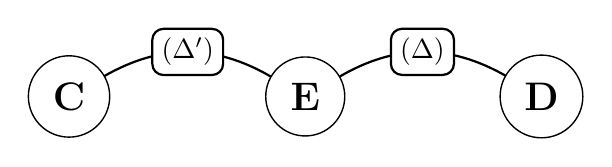
\begin{tikzpicture}
  \SetGraphUnit{3}
  \Vertex{E}
  \WE(E){C}
  \EA(E){D}
  \Edge[label = $(\Delta')$](C)(E)
  \Edge[label = $(\Delta)$](E)(D)
\end{tikzpicture}
\end{center}

where the strict transforms of $C$ and $D$ are still called $C$ and $D$, and $E$ is the inverse image of $x$.

\item if $e$ is a loop, i.e. $x$ belongs to only one component $L$ of $X_s$, then $\Gamma'$ is obtained from $\Gamma$ by replacing $e$ by a cycle

\begin{center}
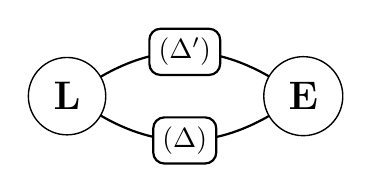
\begin{tikzpicture}
  \SetGraphUnit{3}
  \Vertex{L}
  \EA(L){E}
  \Edge[label = $(\Delta')$](L)(E)
  \Edge[label = $(\Delta)$](E)(L)
\end{tikzpicture}
\end{center}

where the strict transform of $L$ is still called $L$ and $E$ is the inverse image of $x$.

\end{itemize}


\end{lem}

\begin{proof}
The ideal sheaf of $\sigma$ is already Cartier above the smooth locus of $X/S$ and outside the image of $\sigma$, so by the universal property of blow-ups (\cite[\href{https://stacks.math.columbia.edu/tag/0806}{Tag 0806}]{stacks-project}), we only need to describe $\phi$ above the  \'etale localizations $\spec\O_{X,x}^{\on{et}}$, where $x,s,(C,D)$ are as in the statement of the lemma. We can assume $S=\spec R$ is strictly local, with closed point $s$. Pick an isomorphism
\[
\widehat{\O_{X,x}^{\on{et}}}=\widehat{R}[[u,v]]/(uv-\Delta\Delta')
\]
such that $C$ is locally given by $u=0$. The map
\[
\widehat{\sigma}\colon\widehat{\O_{X,x}^{\on{et}}}\ra\widehat{R}
\]
yielded by $\sigma$ sends $u$ to a generator of $\Delta \widehat R$ and $v$ to a generator of $\Delta' \widehat R$. Scaling $u$ and $v$ by a unit of $\widehat R$ if necessary, we can assume $\widehat{\sigma}(u)=~\Delta$ and $\widehat{\sigma}(v)=~\Delta'$.

The completed local rings of $\spec \O_{X,x}^{\on{et}}\times_X X'$ can be computed using the blowing-up of the algebra $B:=R[u,v]/(uv-\Delta\Delta')$ in the ideal $(u-\Delta,v-\Delta')$ (since the completion of $B$ at $(u,v,\m_R)$ is $\widehat{\O_{X,x}}$).
	
	The latter is covered by two affine patches:
	
	\begin{itemize} 
	
	\item the patch where $u-\Delta$ is a generator, given by the spectrum of
	\[
	R[u,v,\alpha]/((v-\Delta')-\alpha(u-\Delta),u\alpha+\Delta')\simeq R[u,\alpha]/(u\alpha+\Delta')
	\]
	since, in the ring $R[u,v,\alpha]/((v-\Delta')-\alpha(u-\Delta))$, the element $uv-\Delta\Delta'$ is equal to $(u-\Delta)(u\alpha+\Delta')$
	
	\item and the patch where $v-\Delta'$ is a generator, where we obtain symmetrically the spectrum of
	\[
	R[v,\beta]/(v\beta+\Delta)
	\]
	\end{itemize}
	with the obvious gluing maps. Thus we see that $X'$ remains nodal, and that the edge $e$ of $\Gamma$ (of label $(\Delta\Delta')$) is replaced in $\Gamma'$ by a chain of two edges, one labelled $(\Delta)$ and one labelled $(\Delta')$. It also follows from this description that the strict transform of $C$ (resp. $D$) in $X'\times_X \spec\widehat{\O_{X,x}^{\on{et}}}$ contains the singularity of label $(\Delta')$ (resp. $(\Delta)$).
\end{proof}

\begin{cor}\label{corollary:unicite_zariski_locale_des_T-refinements}
With the same hypotheses and notations as in Lemma \ref{structure des (C,delta)-blowups}, for any two sections $\sigma,\sigma'$ of $X/S$, the blow-ups $Y\to X$ and $Y'\to X$ in the respective ideal sheaves of $\sigma$ and $\sigma'$ are canonically isomorphic above the same type locus of $\sigma$ and $\sigma'$ in $X$.
\end{cor}

\begin{proof}
It suffices to exhibit, for any point $s\to S$ and any singular point $x$ of $X_s$ such that $\sigma(s)=\sigma'(s)=x$ and $\sigma,\sigma'$ have the same type $T$ at $x$, a Zariski neighbourhood $V$ of $x$ in $X$ and an isomorphism $Y\times_X V \to Y'\times_X V$ compatible with the canonical identifications $Y\times_X X^{sm}=X^{sm}=Y'\times_X X^{sm}$. Since $X,Y,Y'$ are of finite presentation over $S$, this can be done assuming $S=\spec R$ is strictly local, with closed point $s$. Using the universal property of blow-ups (\cite[\href{https://stacks.math.columbia.edu/tag/0806}{Tag 0806}]{stacks-project}), we reduce to proving that the pull-back of the ideal sheaf of $\sigma'$ (resp. $\sigma$) to $Y$ (resp. $Y'$) is Cartier. The proofs are symmetric, so we will only show that the pull-back to $Y$ of the ideal sheaf of $\sigma'$ is Cartier. This, in turn, reduces to proving that the ideal sheaf of $\sigma'$ in $\spec\widehat{\O_{X,x}^{\on{et}}}$ becomes Cartier in $Y\times_X \spec\widehat{\O_{X,x}^{\on{et}}}$. Pick an isomorphism
\[
\widehat{A}:=\widehat{R}[[u,v]]/(uv-\Delta_x)=\widehat{\O_{X,x}^{\on{et}}},
\]
where $\Delta_x\in R$ is a generator of the singular ideal of $x$. The map
\[
\widehat A \to \widehat{R}
\]
corresponding to $\sigma$ sends $u,v$ to elements $\Delta,\Delta'$ of $\widehat{R}$ with $\Delta\Delta'=\Delta_x$. Since $\sigma$ and $\sigma'$ have the same type at $x$, there is a unit $\lambda\in\widehat{R}^\times$ such that the map
\[
\widehat A \to \widehat{R}
\]
corresponding to $\sigma'$ sends $u$ and $v$ to $\lambda\Delta$ and $\lambda^{-1}\Delta'$ respectively. We have reduced to proving that the sheaf given by the ideal $(u-\lambda\Delta, v-\lambda^{-1}\Delta')$ of $\widehat A$ becomes Cartier in the blow-up of $\widehat{A}$ in $(u-\Delta,v-\Delta')$. Put
\[
A=\widehat{R}[u,v]/(uv-\Delta\Delta'),
\]
then it is enough to prove that the ideal $I=(u-\lambda\Delta, v-\lambda^{-1}\Delta')$ of $A$ becomes invertible in the two affine patches (as described in the proof of Lemma \ref{structure des (C,delta)-blowups}) forming the blowing-up of $A$ in $(u-\Delta,v-\Delta')$. By symmetry, we only check it in the patch generated by $u-\Delta$, which is the spectrum of
\[
A_1=\widehat{R}[u,\alpha]/(u\alpha+\Delta'),
\]
where $v$ maps to $\Delta'+\alpha(u-\Delta)$. We have $I=(u-\lambda\Delta,\lambda v-\Delta')$, and in $A_1$ we can write
\begin{align*}
\lambda v -\Delta' & = \lambda (\Delta'+\alpha(u-\Delta)) +u\alpha \\
& = -\lambda\alpha\Delta+u\alpha \\
& = \alpha(u-\lambda\Delta).
\end{align*}
Thus, the preimage of $I$ in $A_1$ is the invertible ideal $(u-\lambda\Delta)$, and we are done.
\end{proof}


\subsection{Resolutions of nodal curves}

\begin{lem}\label{lemme les raffinements font baisser la complexite}
Let $\Gamma,\Gamma'$ be two labelled graphs over a free commutative semigroup. If $\Gamma'\preceq\Gamma$ (Definition \ref{definition refinements of graphs}), then $n_{\Gamma'}\leq n_\Gamma$. If $\Gamma'\prec\Gamma$, then $n_{\Gamma'}< n_\Gamma$.
\end{lem}

\begin{proof}
Suppose $\Gamma'\preceq\Gamma$. Then, by definition, the sum of lengths of edges of $\Gamma$ is equal to the sum of lengths of edges of $\Gamma'$ and $\Gamma'$ has at least as many edges as $\Gamma$, so $n_{\Gamma'}\leq n_\Gamma$.

If equality holds in the latter, then $\Gamma'$ and $\Gamma$ have the same number of edges, which, combined with the fact $\Gamma'\preceq\Gamma$, implies they are isomorphic.
\end{proof}

Now we want, starting from $X$, to find a model of $X_U$ "refining $\Gamma_s$ as much as possible", in the sense that it will be of arithmetic complexity $0$ at $s$ and its dual graph will be a refinement of $\Gamma_s$. We do it following the ideas of \cite{DeJong}, proposition 3.6, as follows:

\begin{defi}\label{definition resolutions}
	Let $X$ be a nodal curve over a regular scheme $S$, smooth over a dense open subscheme $U\subset S$. Let $s$ be a point of $S$. We call \emph{resolution of $X$ at $s$} any nodal $S$-model $X'$ of $X_U$, obtained by a finite sequence of refinements, and of arithmetic complexity $0$ at $s$. If $S$ is strictly local, we call \emph{resolution of $X$} any resolution of $X$ at the closed point.
\end{defi}

\begin{prop}\label{proposition existence des resolutions}
	With the same notations and hypotheses as above, if $S$ is an admissible neighbourhood of $s$, then $X$ admits a resolution at $s$.
\end{prop}

\begin{proof}
For a nodal model $Y$ of $X_U$, write $n_Y$ for the arithmetic complexity of $Y$ at $s$. If $Y \to X$ is a refinement, then $S$ is still an admissible neighbourhood of $s$ relatively to $Y/S$. Let $X'\ra X$ be a finite sequence of refinements minimizing $n_{X'}$, then $X'\ra X$ is a resolution. Indeed, suppose it was not, then there would be a closed singular point $x$ of $X'$ of arithmetic complexity $\geq 1$. There would exist a type $T$ at $x$, and a $T$-refinement $X''\to X$. We would have $n_{X''}<n_{X'}$, a contradiction.
\end{proof}

\begin{rem}
Resolutions are not unique in general. For example, consider $S=~\spec\C[[u,v]]$, and suppose $X$ is a nodal curve over $S$ with dual graph

\begin{center}
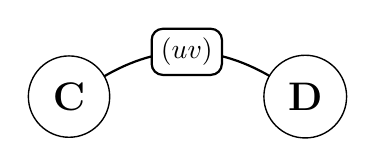
\begin{tikzpicture}
  \SetGraphUnit{3}
  \Vertex{D}
  \WE(D){C}
  \Edge[label = $(uv)$](C)(D)
\end{tikzpicture}
\end{center}

There are two types at the closed singular point $x$ of $X/S$ with respect to $(C,D)$, namely the class $T$ of $u$ and the class $T'$ of $v$. The $T$-refinement and the $T'$-refinement of $X$ are both resolutions, but they are not isomorphic as models of $X_U$ (they are not even isomorphic as schemes as soon as $C,D$ are not isomorphic, e.g. of distinct genera).
\end{rem}


\part{N\'eron models of nodal curves and their Jacobians}\label{part2}

\section{Generalities about N\'eron models}\label{Generalities_about_NMs}

\subsection{Definitions}

\begin{defi}
	Let $S$ be a scheme and $U$ a scheme-theoretically dense open subscheme of $S$. Let $Z/U$ be a $U$-algebraic space. An \textit{$S$-model} of $Z$ (or just \textit{model} if there is no ambiguity) is an $S$-algebraic space $X$ together with an isomorphism $X_U=Z$. A \textit{morphism of $S$-models} between two models $X$ and $Y$ of $Z$ is an $S$-morphism $X\ra Y$ that commutes over $U$ with the given isomorphisms $X_U=Z$ and $Y_U=Z$.
\end{defi}

\begin{defi}\label{definition:neron_models}
	Let $S$ be a scheme and $U$ a scheme-theoretically dense open subscheme of $S$. Let $Z/U$ be a smooth $U$-scheme. A \textit{$S$-Néron model} of $Z$ (or just \textit{Néron model} if there is no ambiguity) is a smooth $S$-model $N$ satisfying the following universal property, called the \textit{Néron mapping property}:
	
For each smooth $S$-algebraic space $Y$, the restriction map \[
\Hom_S(Y,N)\ra\Hom_U(Y_U,Z)
\]
is bijective.
\end{defi}

\begin{rem}
In the litterature, N\'eron models are often required to be separated and of finite type over the base. Néron models without a quasi-compactness condition are sometimes referred to as N\'eron-lft models, where "lft" stands for "locally of finite type". We justify the definition above by observing that our Néron models are still unique up to a unique isomorphism by virtue of the universal property: we can always discuss their separatedness or quasi-compactness a posteriori.
\end{rem}

\begin{rem}
	Let $S$, $U$, $Z$ be as above, and $N$ be a smooth, separated $S$-model of $Z$. Consider a smooth $S$-algebraic space $Y/S$ and two morphisms $f_1,f_2\colon Y\ra N$ that coincide over $U$. The separatedness of $N/S$ implies that the equalizer of $f_1$ and $f_2$ is a closed subspace of $Y$ containing $Y_U$, and the latter is scheme-theoretically dense in $Y$ by \cite[Théorème 11.10.5]{EGA4.3}. Thus, we automatically have \emph{uniqueness in the N\'eron mapping property for $N/S$}, i.e. injectivity of the restriction map
	\[
	\Hom_S(Y,N) \to \Hom_U(Y_U,Z).
	\]
In particular, a separated $S$-space satisfying existence in the N\'eron mapping property (i.e. surjectivity of the restriction map) is automatically the Néron model.
\end{rem}


\begin{rem}\label{remark:NMs_represent_the_restriction_functor_on_small_smooth_site}
By descent, Definition \ref{definition:neron_models} is unchanged if we only require the Néron mapping property to hold when $Y/S$ is a scheme. Therefore, when we ask if a Néron model exists for $X_U/U$, we are asking if the functor $Y \mapsto X_U(Y_U)$ on the small smooth site of $S$ is representable by a smooth algebraic space. Similarly, we would get a looser (but still universal) definition of Néron models by asking for them to be smooth algebraic stacks.
\end{rem}

\subsection{Base change and descent properties}




\begin{prop}[The formation of Néron models is compatible with smooth base change]\label{changement de base lisse}
Consider a smooth morphism $S'\ra S$, a scheme-theoretically dense open $U\subset S$ and a smooth $S$-model $X$ of $X_U$ with uniqueness in the Néron mapping property. Then, the base change $X_{S'}$ is a smooth $S'$-model of $X_{U'}$ with uniqueness in the Néron mapping property. If $X$ is the Néron model of $X_U$, then $X'$ is the Néron model of $X_{U'}$.
\end{prop}

\begin{proof}
	First, note that $X_{S'}/S'$ is smooth since $X/S$ is, and that $U'$ is scheme-theoretically dense in $S'$ by \cite{EGA4.3}, théorème 11.10.5. Thus, we only need to check that $X'/S'$ has uniqueness in the Néron mapping property, and existence if $X/S$ does.

	Let $Y'$ be a smooth $S'$-scheme. A morphism $Y' \to X'$ is uniquely determined by the two projections $Y' \to S'$ and $Y' \to X$. Since $Y' \to S$ is smooth, it follows that $X'$ has uniqueness in the Néron mapping property. Now, suppose that $X$ is the Néron model of $X_U$ and consider a $U'$-morphism $u': Y'_{U'}\ra X_{U'}$. Composing with the projection: $X_{U'}\ra X_U$, we get a $U$-morphism $Y'_{U'}\ra X_U$, which extends to a unique $S$-morphism $Y'\ra X$ by the Néron mapping property since $Y'/S$ is smooth. Then the induced morphism $Y'\ra X'$ extends $u'$.
\end{proof}

\begin{cor}\label{corollaire le NM passe aux limites d'algebres lisses}
	If $S'/S$ is a cofiltered limit of smooth $S$-schemes (indexed by a cofiltered partially ordered set, e.g. a localization, a henselization when $S$ is local...), and $X$ is the $S$-Néron model of $X_U$, then $X_{S'}$ is the $S'$-Néron model of $X_{U'}$.
\end{cor}

\begin{lem}[N\'eron models are compatible with disjoint unions on the base]\label{lemma:neron_models_compatible_with_disjoint_unions}
Let $I$ be a set, $(S_i)_{i\in I}$ a family of schemes, and $(N_i \to S_i)_{i\in I}$ a family of morphisms of algebraic spaces. Write $S=\coprod\limits_{i\in I}S_i$ and $N=\coprod\limits_{i\in I}N_i$. Let $U$ be a scheme-theoretically dense open of $S$, and write $U_i=U\times_S S_i$ for every $i$. Then $N$ is the $S$-N\'eron model of $N_U$ if and only if for all $i$ in $I$, $N_i$ is the $S_i$-N\'eron model of $N_i\times_{S_i} U_i$.
\end{lem}

\begin{proof}
Suppose $N$ is the N\'eron model of $N_U$. Then, by Proposition \ref{changement de base lisse}, for all $i$ in $I$, $N_i$ is the N\'eron model of $N_i\times_{S_i}U_i$. Conversely, suppose that for every $i$ in $I$, $N_i/S_i$ is the N\'eron model of its restriction to $U$, and consider a smooth $S$-algebraic space $Y$ with a morphism $f_u\colon Y_U \to N_U$. For each $i$, we write $Y_i=Y\times_S S_i$. We have
\begin{align*}
\Hom_S(Y,N) & = \prod\limits_{i\in I} \Hom_{S_i}(Y_i,N_i)\\
& = \prod\limits_{i\in I} \Hom_{U_i}(Y_i\times_{S_i} U_i, N_i\times_{S_i} U_i)\\
& = \Hom_U(Y_U, N_U),\\
\end{align*}
where the second equality holds because each $Y_i/S_i$ is smooth. Since $N/S$ is smooth if and only if all the $N_i/S_i$ are smooth, we are done.
\end{proof}


\begin{prop}[N\'eron models descend along smooth covers]\label{proposition descente lisse du NM}
	Let $S$ be a scheme and $U$ a scheme-theoretically dense open of $S$. Let $S'\ra S$ be a smooth surjective morphism and $U'=U\times_S S'$. Let $X_U$ be a smooth $U$-algebraic space, and let $X'$ be a smooth $S'$-model of $X_{U'}$. Suppose $X'$ has uniqueness in the Néron mapping property, then it comes via base-change from a smooth $S$-model $X$ of $X_U$ with uniqueness in the Néron mapping property. If $X'$ is the Néron model of $X_{U'}$, then $X$ is the Néron model of $X_U$.
\end{prop}

\begin{proof}
Call $p_1,p_2$ the two projections $S'':=S'\times_S S'\ra S'$. They are smooth morphisms, so by Proposition \ref{changement de base lisse} and uniqueness in the Néron mapping property, we know $p_1^*X'=p_2^*X'$ as both coincide over $U''=U\times_S S''$. By the effectiveness of fppf descent for algebraic spaces (\cite[\href{https://stacks.math.columbia.edu/tag/0ADV}{Tag 0ADV}]{stacks-project}), $X'$ comes via base change from an $S$-algebraic space $X/S$.

The morphism $X\ra S$ is smooth since $X'/S'$ is (smoothness is even fpqc local on the base, see \cite[\href{http://stacks.math.columbia.edu/tag/02VL}{Tag 02VL}]{stacks-project}). Therefore, we only need to prove that $X/S$ has uniqueness in the Néron mapping property, and existence if $X'$ does. Take $Y$ a smooth $S$-algebraic space, and let
\[
f,g\colon Y \longrightarrow X
\]
be two morphisms that coincide over $U$. Then the pull-backs of $f$ and $g$ by $S' \to S$ coincide over $U'$, hence are equal. Since $S' \to S$ is a cover, we have $f=g$.
Now, suppose $X'$ is a Néron model and consider a generic morphism $f_U\colon Y_U\ra X_U$. Write $Y'$ (resp. $f'_U$) for the pullback of $Y$ (resp. $f_U$) under $S'\ra S$. Then $Y'/S'$ is smooth so $f'_U$ extends to a unique $f'\colon Y'\ra X'$. We have a cartesian diagram
\[
\xymatrix{
Y''\ar@<-.5ex>[d] \ar@<.5ex>[d] \ar@<-.5ex>[r] \ar@<.5ex>[r] &Y'\ar[d]\ar[r] &Y\ar@/^/[dd]\\
X''\ar[d] \ar@<-.5ex>[r] \ar@<.5ex>[r] &X'\ar[d]\ar[r] &X\ar[d]\\
S''\ar@<-.5ex>[r] \ar@<.5ex>[r] &S'\ar[r] &S
}
\]
where $S'':=S'\times_S S'$ and the arrows $S''\ra S'$ are the two projections $p_1,p_2$, so that all horizontal rows are equalizers. We only need to show that $p_1^*f'=p_2^*f'$, which follows from uniqueness in the N\'eron mapping property of $X''/S''$ since they coincide over $U''$.
\end{proof}



\begin{prop}\label{proposition on peut check qu'on est un NM sur les germes etales}
Let $S$ be a scheme, $U\subset S$ a scheme-theoretically dense open subscheme, $X_U/U$ a smooth $U$-scheme and $N/S$ a model of $X_U$ of finite type. Then $N$ is the N\'eron model of $X_U$ if and only if for every point $s\in S$, $N\times_S\spec\O_{S,s}^{\on{et}}$ is the $\spec\O_{S,s}^{\on{et}}$-N\'eron model of its restriction to $U$.
\end{prop}

\begin{proof}
The "only if" part is a special case of Corollary \ref{corollaire le NM passe aux limites d'algebres lisses}. We prove the "if" part. Suppose that for all $s\in S$, $N$ is the N\'eron model over $\spec\O_{S,s}^{\on{et}}$ of its restriction to $U$. Then $N/S$ is smooth at any geometric point, hence smooth. Let $Y/S$ be a smooth $S$-algebraic space and $f_u\colon Y_U\ra X_U$ a $U$-morphism. Since $Y/S$ is locally of finite presentation, by \cite{EGA4.3}, théorème 8.8.2, every point $s\in S$ has an \'etale neighbourhood $V_s\ra S$ such that $f_u$ extends uniquely to a morphism $Y\times_S V_s\ra N\times_S V_s$. By \cite{EGA4.3}, théorème 11.10.5, $U$ remains scheme-theoretically dense in every $V_s$, so these maps glue as in the proof of Proposition \ref{proposition descente lisse du NM} and $f_U$ extends to a morphism $Y\ra N$.
\end{proof}


\subsection{Group models with injective restriction map}

In this subsection, we show that any smooth group model of a group algebraic space has a biggest quotient with uniqueness in the Néron mapping property, namely the quotient by the étale part of its unit section (Corollary \ref{corollary:quotient_of_group_space_by_E^et_has_uniqueness_in_NMP}). Given a scheme $S$, we will write $\sm S$ (resp. $\schsm S$) for the small smooth site (resp. big smooth site) of $S$.

We write $\ab$ for the category of abelian groups. We will use without further mention the fact that a smooth $S$-algebraic space is determined up to a unique isomorphism by the corresponding functor $(\sm S)^{\on{op}} \to \ab$ (by combining the Yoneda lemma with a descent argument).

\begin{defi}
Let $S$ be a scheme and $E/S$ an $S$-algebraic space. We call \emph{étale part of $E$ over $S$} the union $E^{\on{et}/S}$ of all open subspaces of $E$ that are étale over $S$. When there is no ambiguity, we simply call it the \emph{étale part of $E$} and write it $E^{\on{et}}$.
\end{defi}

\begin{lem}[\cite{Holmes}, Lemma 5.17]\label{lemma:sections_of_E_factor_through_E^et}
Let $S$ be a scheme, $U\subset S$ a scheme-theoretically dense open and $f\colon E \to S$ a $S$-algebraic space. Suppose that $f$ restricts to an isomorphism over $U$ and that $U\times_S E$ is scheme-theoretically dense in $E$. Then any section of $f$ factors through $E^{\on{et}}$.
\end{lem}

\begin{proof}
The claim is étale-local on $S$ and $E$, so we may assume that $f$ is a morphism of affine schemes. In particular, $f$ is separated. Then $S \to E$ is a closed immersion through which $U$ factors, hence an isomorphism. A fortiori, $f$ is étale.
\end{proof}

\begin{cor}\label{corollary:quotient_of_group_space_by_E^et_has_uniqueness_in_NMP}
Let $S$ be a scheme, $U\subset S$ a scheme-theoretically dense open subscheme, $N_U \to U$ a smooth, separated $U$-group algebraic space and $f\colon N \to S$ a smooth $S$-group model of $N_U$. Call $E$ the scheme-theoretical closure of the unit section in $N$. Then, for any smooth $S$-scheme $Y$, the sequence of abelian groups
\[
0 \to \Hom(Y,E^{\on{et}}) \to \Hom(Y,N) \to \Hom(Y_U,N_U)
\]
is exact. In particular, the quotient space $N/E^{\on{et}}$ is a smooth $S$-group model of $N_U$ with uniqueness in the Néron mapping property.
\end{cor}

\begin{rem}
In the setting of Corollary \ref{corollary:quotient_of_group_space_by_E^et_has_uniqueness_in_NMP}, if $N$ has existence in the Néron mapping property, it follows that $N/E^{\on{et}}$ is the Néron model of $N_U$.
\end{rem}

%\begin{prop}\label{proposition:finitely_many_group_models_map_to_common_model_with_uniqueness_in_NMP}
%Let $S$ be a scheme, $U\subset S$ a scheme-theoretically dense open subscheme and $N_U/U$ a smooth, separated $U$-group algebraic space. Let $I$ be a finite set. For all $i\in I$, let $V_i \to S$ be a smooth morphism of schemes and $N_i \to V_i$ be a smooth group $S$-model of $(N_U\times_S V_i)/(U\times_S V_i)$. Let $F$ be the sheafification of the presheaf on $(\sm S)^{\on{op}}\to\ab$ sending $Y/S$ to the sum of the images of the $\Hom(Y,N_i)$ in $\Hom(Y_U,N_U)$. Then $F$ is representable by a smooth $S$-group algebraic space $N$.
%\end{prop}

%\begin{proof}
%Using Corollary \ref{corollary:quotient_of_group_space_by_E^et_has_uniqueness_in_NMP}, we may assume each $N_i/V_i$ has uniqueness in the Néron mapping property. By Proposition \ref{proposition descente lisse du NM}, we may assume each $V_i\to S$ is an open immersion. Replacing each $N_i$ by the gluing of $N_i$ with $N_U$ along their (canonically isomorphic) open subspaces $N_i\times_S U=N_U\times_S V_i$, we may assume $V_i=S$ for every $i$.

%We write $\bigtimes$ for the fiber product over $S$. Let $K$ be the kernel of the multiplication $\bigtimes\limits_{i\in I} N_U \to N_U$. Call $\overline N$ the quotient $\left(\bigtimes\limits_{i\in I}N_i\right)/K$ (which is an algebraic space since $K$ is $S$-flat). Then $\overline N$ is a smooth $S$-group model of $N_U$. For any $j\in I$, the composition
%\[
%N_j \to \bigtimes\limits_{i\in I}N_i \to \overline N
%\]
%is a morphism of models of $N_U$ (where $N_j$ maps to the factor $\bigtimes\limits_{i\neq j}N_i$ via the zero map). Hence, applying Corollary \ref{corollary:quotient_of_group_space_by_E^et_has_uniqueness_in_NMP}, we find that the quotient of $\overline{N}$ by the étale part of the closure of its unit section represents $F$.
%\end{proof}


\section{N\'eron models of Jacobians}\label{sec6}

If $X\to S$ is a morphism of schemes, its relative Picard functor is the fppf sheafification of the functor sending a $S$-scheme $T$ to the group of isomorphism classes of line bundles on $X_T$. When $X/S$ is a nodal curve, by \cite[Theorem 8.3.1; Theorem 9.4.1]{NeronModels} the Picard functor is representable by a smooth, quasi-separated $S$-group algebraic space $\pic_{X/S}$, the \emph{Picard space}. We write $\pic^{\on{tot}0}_{X/S}$ for the kernel of the degree map from $\pic_{X/S}$ to the constant sheaf $\Z$ on $S$; and $\pic^{0}_{X/S}$ for the fiberwise-connected component of identity of $\pic_{X/S}$, parametrizing line bundles of degree $0$ on every irreducible component of every fiber.

A classical way of obtaining a N\'eron model for the Jacobian $J$ of a proper smooth curve $X_U/U$ with a nodal model $X/S$, when $X$ is "nice enough", is to consider the quotient $P/E$, where $P=\pic^{\on{tot}0}_{X/S}$ and $E$ is the closure of the unit section in $P$, so that $P/E$ is the biggest separated quotient of $P$ (see for example \cite[9.5]{NeronModels}). This works well when three conditions are met: $P$ is representable by an $S$-algebraic space; $E$ is flat over $S$ (so that the quotient is also representable); and $\pic^{\on{tot}0}_{X/S}$ satisfies existence in the N\'eron mapping property (e.g. $X$ is regular). However, this approach fails most of the time when $S$ is of arbitrary dimension, since $E$ is rarely $S$-flat (\cite[Theorem 5.16]{Holmes}). The reason is that this method is designed to produce \emph{separated} Néron models, and most Néron models over higher-dimensional bases turn out to be non-separated.

In this section, we will work assuming $S$ is a regular scheme and $U\subset S$ a dense open subscheme. In view of Corollary \ref{corollary:quotient_of_group_space_by_E^et_has_uniqueness_in_NMP}, it is tempting to try to construct the Néron model as the quotient of $P$ by the étale part of $E$. This works when $P$ has existence in the Néron mapping property, i.e. when $X$ is parafactorial along $X_U$ after any smooth base change (e.g. regular). However, even if $X_U$ has nodal models, it may be that none of them remains parafactorial after every smooth base change. We will show that such a model exists after passing to some étale cover of the base, from which it follows by descent that the Néron model exists. We will give a simple combinatorial criterion for the Néron model to be separated, related to the alignment condition of \cite{Holmes}.


\subsection{Construction of the Néron model}



\begin{prop}\label{proposition:nodal_curves_have_quasi_resolutions}
Let $S$ be a regular scheme, $U\subset S$ a dense open subscheme and $X/S$ a nodal curve, smooth over $U$. There exist morphisms of schemes $V \to S$ and $X'\to X_V$ such that
\begin{itemize}
\item $V \to S$ is an étale cover.
\item $X'/V$ is a nodal model of $X_U\times_S V$.
\item For any geometric point $s \to S$, there exists a geometric point $v \to V$ above $s$ such that the singular ideals of $X'$ at $v$ are prime in $\O_{V,v}^{\on{et}}$.
\end{itemize}
\end{prop}

\begin{proof}
For any point $s\in S$, pick an admissible neighbourhood $V^s$ of $s$ (Definition \ref{definition:admissible}) and a resolution $X^s$ of $X$ (Proposition \ref{proposition existence des resolutions}). Then $V=\coprod\limits_{s\in S} V^s$ and $X'=\coprod\limits_{s\in S} X^s$ satisfy all three conditions.
\end{proof}

\begin{thm}\label{theorem:NMs_of_jacobians}
Let $S$ be a regular scheme, $U\subset S$ a dense open subscheme and $X/S$ a nodal curve, smooth over $U$. Then, the Jacobian $J$ of $X_U$ admits a Néron model $N$ over $S$. Moreover, there exists an étale cover $V \to S$ such that $N_V$ is of the form $\pic^{\on{tot}0}_{X'/V}/E^{\on{et}}$, where $X'/V$ is a nodal model of $X_U\times_S V$ and $E$ is the closure of the unit section in $\pic^{\on{tot}0}_{X'/V}$.
\end{thm}

\begin{proof}
We may assume that $X/S$ has a section. Let $V \to S$ and $X' \to X_V$ be as in Proposition \ref{proposition:nodal_curves_have_quasi_resolutions}, and put $P=\pic^{\on{tot}0}_{X'/V}$. By Proposition \ref{proposition descente lisse du NM} and Corollary \ref{corollary:quotient_of_group_space_by_E^et_has_uniqueness_in_NMP}, the quotient $P/E^{\on{et}}$ comes via base change from a $S$-group model $N$ of $J$ with uniqueness in the Néron mapping property. Let $Y$ be a smooth $S$-scheme, we will show that any morphism $f_U\colon Y_U \to J$, extends to a morphism $Y \to N$. By uniqueness in the Néron mapping property for $N$, it suffices to extend $f_U$ étale-locally on $Y$ around an arbitrary geometric point $y \to Y$. By Corollary \ref{corollary:irred_of_etale_loc_ring_stable_under_smooth_maps}, and by the definition of $X'$, there is an étale neighbourhood $Y'$ of $y$ in $Y\times_S V$ such that the singular ideals of $X'\times_V Y'$ at $y$ are prime. By Lemma \ref{les anneaux locaux sont UFD} and Lemma \ref{lemme les irreductibles au complete sont les irreductibles}, shrinking $Y'$, we may assume that $X'\times_V Y'$ is locally factorial. Hence, the generic line bundle corresponding to $f_U$ extends to a line bundle on all of $X'\times_V Y'$, which gives a morphism $Y' \to P$. Composing with $P \to P/E^{\on{et}} \to N$, we obtain a morphism $Y' \to N$ extending $f_U$.
\end{proof}

\begin{rem}\label{remark:can_glue_local_models_of_curves_on_each_stratum}
In the proof above, the quotients of the Picard spaces of the $X^s/V^s$ by the étale parts of the closures of their respective unit sections naturally glue in the étale topology into a $S$-space, but the $X^s$ themselves do not necessarily glue. However, we could glue them into a locally finite number of local models with similar properties as follows.

Consider the relation $R$ on $S$ given by $sRt$ whenever $t$ specializes $s$ and for some (equivalently, any) geometric points $\bar t$ above $t$ and $\bar s$ above $s$, the restriction map of étale stalks induces a canonical isomorphism between prime factors of singular ideals of $X$ at $\bar t$ and at $\bar s$. Call $\sim$ the transitive closure of $R$, then it follows from \cite[Corollaire 9.7.10]{EGA4.3} that the equivalence classes for $\sim$ are locally constructible subsets of $S$. In particular, they are locally in finite number. Suppose $X/S$ is orientable everywhere and admits a family of orientations at every singular point compatible with the generization isomorphisms of Lemma \ref{lemma:orientations_pass_to_generization} (which holds on some étale cover of $S$). For any equivalence class $F$ of $\sim$, using Corollary \ref{corollary:unicite_zariski_locale_des_T-refinements}, we can find an étale morphism $\pi\colon V \to S$ whose image contains $F$, and a nodal model of $X_U$ over $V$ whose singular ideals at \emph{every} singular point above $F$ are prime.
\end{rem}


\begin{rem}\label{remark:strict_log_jac_vs_pic_aggregate}
In \cite{HMOPModelsJacobians}, the authors describe the \emph{strict logarithmic Jacobian} of a logarithmic curve, an algebraic space with a moduli interpretation. They show that when $X/S$ is a nodal curve over a toroidal variety, smooth over the complement $U$ of the boundary divisor, then there are canonical log structures on $X$ and $S$ such that the strict logarithmic Jacobian is the Néron model of $X_U$. In particular, this gives a moduli interpretation for the Néron model constructed in Theorem \ref{theorem:NMs_of_jacobians} when $U$ is the complement in $S$ of a divisor with normal crossings. The same holds when $U\subset S$ is arbitrary. Indeed, let $M_S$ be the étale subsheaf of monoids of $\O_S$ whose étale stalks are generated by the units and by the prime factors of the singular ideals of $X$. Let $M_X$ be the submonoid of $\O_X$ whose étale stalk at a geometric point $x\to X$ above a geometric point $s\to S$ is:
\begin{itemize}
\item The submonoid of $\O_{X,x}^{\on{et}}$ spanned by $(\O_{X,x}^{\on{et}})^\times$ and $M_{S,s}$ if $x$ is smooth over $S$.
\item The submonoid of $\O_{X,x}^{\on{et}}$ spanned by $(\O_{X,x}^{\on{et}})^\times$, $M_{S,s}$ and local parameters for the two branches of $X/S$ at $x$ if $x$ is singular.
\end{itemize}
Then, $M_S\to \O_S$ and $M_X\to \O_X$ are logarithmic structures in the sense of \cite{Kato}, but they do not necessarily admit étale-local charts (cf example \ref{example:irred_not_etale_irred}). Therefore, $(X,M_X)\to (S,M_S)$ is not a logarithmic curve in the sense of \cite{HMOPModelsJacobians}. However, replacing $U$ by the maximal open subscheme of $S$ over which $X$ is smooth, i.e. on which $M_S=\O_S^\times$, we find that the groupification $M_X^{gp}$ coincides with the direct image of $\O_{X_U}^\times$ in $X$. Hence, two isomorphism classes of $M_X^{gp}$-torsors which coincide over $X_U$ are equal. Write $H^1(X,M_X^{gp})^\dagger$ for the subgroup of $H^1(X,M_X^{gp})$ consisting of torsors which, locally on $S$, come from a line bundle on a refinement of $X$. Then it follows that $H^1(X,M_X^{gp})^\dagger=\Hom(U,\pic^0_{X_U/U})$. Combining this with the fact that the formation of $M_S$ and $M_X$ commutes with smooth base change by Corollary \ref{corollary:irred_of_etale_loc_ring_stable_under_smooth_maps}, we find that
\begin{align*}
(\sch/S)^{\on{op}} & \to \set \\
T & \mapsto H^1(X,M_X^{gp})^\dagger
\end{align*}
is the Hom functor of the Néron model of $\pic^0_{X_U/U}$.
\end{rem}


\subsection{A criterion for separatedness}

In this subsection, we exhibit a necessary and sufficient combinatorial condition for the Néron model of Theorem \ref{theorem:NMs_of_jacobians} to be separated, closely related to the alignment condition of \cite{Holmes}.

\begin{defi}\label{c-strict alignment}
	Suppose $S$ is a regular scheme. Let $s$ be a geometric point of $S$ and $R=\O_{S,s}^{\on{et}}$. Following \cite{Holmes}, Definition 2.11, we say that a labelled graph $\Gamma$ is \textit{aligned} when for every cycle $\Gamma^0$ in $\Gamma$, all the labels figuring in $\Gamma^0$ are positive powers of the same principal ideal; and that a nodal curve $X/S$ is \textit{aligned at $s$} when its dual graph $\Gamma_s$ at $s$ is aligned. We say $X/S$ is \emph{aligned} if it is aligned at every geometric point of $S$.

	We say that $\Gamma_s$ is \textit{strictly aligned}, or that $X$ is \textit{strictly aligned at $s$}, when it satisfies the following condition: for any cycle $\Gamma^0\subset\Gamma_s$, there exists a \emph{prime} element $\Delta\in R$ such that all the labels of $\Gamma^0$ are powers of the principal ideal $(\Delta)$ of $R$. We say that $X$ is \textit{strictly aligned} if it is strictly aligned at every geometric point of $S$.
\end{defi}

\begin{ex}
Over $S=\spec\C[[u,v]]$, at the closed point, among the three following dual graphs, the first is not aligned; the second is aligned but not strictly, and the third is strictly aligned.

\begin{center}
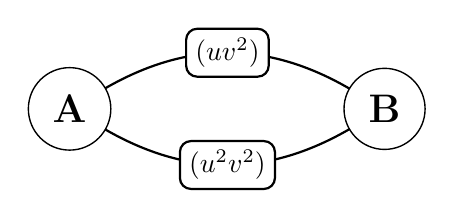
\begin{tikzpicture}
  \SetGraphUnit{4}
  \Vertex{B}
  \WE(B){A}
  \Edge[label = $(uv^ 2)$](A)(B)
  \Edge[label = $(u^ 2v^ 2)$](B)(A)
\end{tikzpicture}
\end{center}


\begin{center}
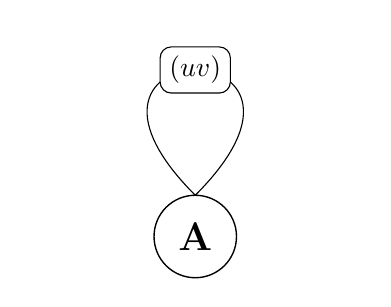
\begin{tikzpicture}
  \SetGraphUnit{4}
  \Vertex{A}
  \Loop[style={}, dist = 3cm, dir = EA, label = $(uv)$](A.north)
\end{tikzpicture}
\end{center}

\begin{center}
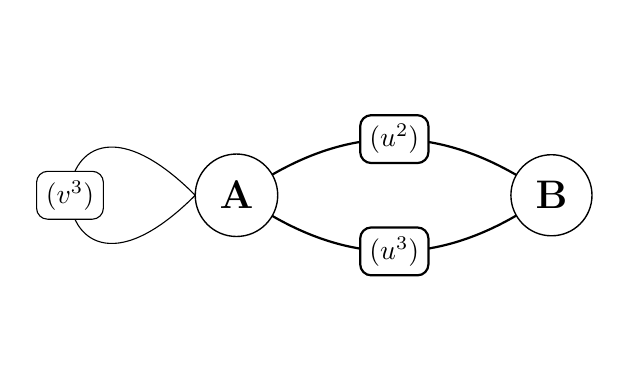
\begin{tikzpicture}
  \SetGraphUnit{4}
  \Vertex{B}
  \WE(B){A}
  \Edge[label = $(u^2)$](A)(B)
  \Edge[label = $(u^3)$](B)(A)
  \Loop[style={}, dist=3cm, dir=NO, label=$(v^3)$](A.west)
\end{tikzpicture}
\end{center}
\end{ex}


	We have to be a little careful about the fact that alignment and strict alignment both deal with étale neighbourhoods. Let us consider two examples.

\begin{ex} The curve over $R=\C[u,v]_{(u,v)}$, given in the weighted projective space $\P_S(1,2,1)$ (in affine coordinates $(x,y)$) by
\[
y^2=\left((x-1)^2-(1+v)v^2+u^2\right)\left((x+1)^2+(1+v)v^2-u^2\right)
\]
is quasisplit, and its dual graph at the closed point is the following 2-gon:

\begin{center}
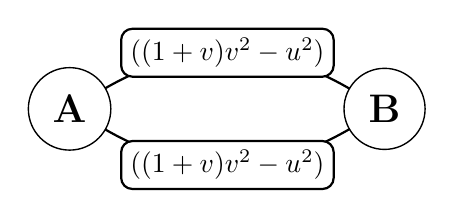
\begin{tikzpicture}
  \SetGraphUnit{4}
  \Vertex{B}
  \WE(B){A}
  \Edge[label = $((1+v)v^2-u^2)$](A)(B)
  \Edge[label = $((1+v)v^2-u^2)$](B)(A)
\end{tikzpicture}
\end{center}

but it is not strictly aligned, even though $((1+v)v^2-u^2)$ is a prime element of $R$. Indeed, $((1+v)v^2-u^2)$ is prime in $R$ but has two distinct prime factors in a strict henselization, since $(1+v)$ becomes a square, and it is the prime factor decomposition in the \'etale local rings that counts in the definition of strict alignment.
\end{ex}

\begin{ex} On the other hand, the equation
\[
y^2=\left((x-1)^2-v^2+u^3\right)\left((x+1)^2+v^2-u^3\right)
\]
defines a nodal curve over $\spec R$ with dual graph

\begin{center}
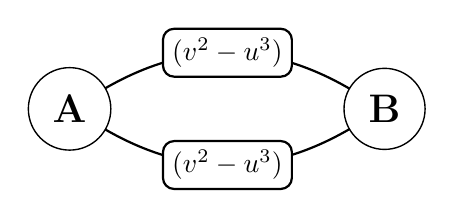
\begin{tikzpicture}
  \SetGraphUnit{4}
  \Vertex{B}
  \WE(B){A}
  \Edge[label = $(v^2-u^3)$](A)(B)
  \Edge[label = $(v^2-u^3)$](B)(A)
\end{tikzpicture}
\end{center}

which is strictly aligned at the closed point, because $v^2-u^3$ remains prime in $R^{sh}$.
\end{ex}

\begin{prop}\label{alignement et platitude de E}
	Let $S$ be a regular scheme, $U\subset S$ a dense open, and $X/S$ a nodal curve, smooth over $U$. Let $P=\pic^{\on{tot}0}_{X/S}$, and $E$ be the scheme-theoretical closure in $P$ of its unit section. Then the following conditions are equivalent:
	
	\begin{enumerate}
		\item $E/S$ is flat.
		\item $E/S$ is \'etale.
		\item $X/S$ is aligned.
	\end{enumerate}
\end{prop}

\begin{proof}
	This is \cite{Holmes}, Theorem 5.17.
\end{proof}

\begin{thm}\label{theorem:separatedness_of_NM_jac_iff_strictly_aligned}
Let $S$ be a regular and excellent scheme, $U\subset S$ a dense open subscheme and $X/S$ a nodal curve, smooth over $U$. Call $J$ the Jacobian of $X_U/U$. Then, the $S$-Néron model $N$ of $J$ exhibited in Theorem \ref{theorem:NMs_of_jacobians} is separated if and only if $X/S$ is strictly aligned.
\end{thm}

\begin{proof}
First, suppose that $N$ is separated. Let $s \to S$ be a geometric point, we will show that $X/S$ is aligned at $s$. Since alignment is an étale-local condition on the base, we may assume that $S$ is an admissible neighbourhood of $s$. Let $Y \to X$ be a resolution of $X$ at $s$, then the closure of the unit section in $\pic^{\on{tot}0}_{Y/S}$ is étale over $S$ by \cite{Holmes}, Theorem 6.2. Hence, $Y$ is aligned at $s$ by Proposition \ref{alignement et platitude de E}. Since the singular ideals of $Y$ at $s$ are prime, it follows that $Y$ is strictly aligned at $s$. By Lemma \ref{structure des (C,delta)-blowups}, it follows that $X$ is strictly aligned at $s$.

Conversely, suppose that $X$ is strictly aligned. We will show that $N$ is separated. Since separatedness is a local property on the target for the étale topology, and since strict alignment is preserved by refinements and étale base change, by Theorem \ref{theorem:NMs_of_jacobians} we may assume that $N$ is the quotient of $P=\pic^{\on{tot}0}_{X/S}$ by the étale part of the scheme-theoretical closure $E$ of its unit section. By Proposition \ref{alignement et platitude de E}, $E$ is étale over $S$, so $N=P/E$ is separated.
\end{proof}




\section{N\'eron models of curves with nodal models}\label{NMs_of_curves_with_nodal_models}

Let $S$ be a regular base scheme, $U$ a dense open subscheme of $S$, and $X/S$ a nodal relative curve, smooth over $U$. In what follows, we are interested constructing and describing the $S$-Néron model of the curve $X_U/U$. 
	
	Under some restrictions on the rational curves appearing in the geometric fibers of $X/S$, we will show that a Néron model $N$ for $X_U$ exists (Theorem \ref{Theorem:ns_neron_models_of_nodal_curves}). When $X/S$ is quasisplit, we will show that if $N$ is separated, then almost all of the connected components of $\sing(X/S)$ are irreducible. We will refine this into a necessary and sufficient condition for the separatedness of $N$ (Theorem \ref{Theorem:separatedness_of_nm_curves}).

%\begin{thm}[Theorem \ref{Theorem:ns_neron_models_of_nodal_curves}]
%Let $S$ be a regular excellent scheme, $U\subset S$ a dense open subscheme and $X/S$ a nodal curve, smooth over $U$, of genus $g\geq 2$. Suppose that $X$ has no rational loops, and suppose that no geometric fiber of $X$ contains a rational component meeting the non-exceptional other irreducible components in three points or more. Then $X_U/U$ has a N\'eron model $N/S$. If in addition $X/S$ is quasisplit, then $N$ is the smooth aggregate (Construction \ref{construction:nodal_aggregate}) of the stable model $X^{stable}$ of $X_U$ (Definition \ref{definition stable model}).
%\end{thm}

%\begin{thm}[Theorem \ref{Theorem:separatedness_of_nm_curves}]
%Let $X/S$ be a nodal curve of genus $\geq 1$, smooth over some dense open $U\subset S$, with $S$ regular and excellent. If $X_U$ has a separated N\'eron model over $S$, then the two following conditions are met:
%\begin{itemize}
%\item The singular locus $\sing(X/S)$ is irreducible around every non-exceptional singular geometric point of $X/S$.
%\item For any geometric point $s\to S$, if a rational component $E$ of $X_s$ meets the non-exceptional other components of $X_s$ in exactly two points $x$ and $y$, then the singular ideals of $x$ and $y$ in $\O_{S,s}^{\on{et}}$ have the same radical.
%\end{itemize}

%Conversely, suppose these conditions are met. Suppose in addition that no geometric fiber of $X/S$ contains either a rational cycle or a rational component meeting the non-exceptional other components in at least three points. Then the N\'eron model of $X_U/U$ exhibited in Theorem \ref{Theorem:ns_neron_models_of_nodal_curves} is separated over $S$.
%\end{thm}



\subsection{Factoring sections through refinements}\label{Factoring sections through refinements}
A first question, easier to tackle than existence of a N\'eron model, is "given a $U$-point of $X_U$, can we extend it to a section of a smooth $S$-model of $X_U$".

We answer with a two-step strategy: first, when $X$ has no rational component in its geometric fibers, all $U$-points of $X$ extend to sections by the following result from \cite{HypersurfacesMovingLemma}:
\begin{prop}[\cite{HypersurfacesMovingLemma}, Proposition 6.2]\label{pas de courbe rationnelle ==> les points rationnels s'étendent en sections}
	Let $X/S$ be a proper morphism of schemes, where $S$ is noetherian, regular and integral. Let $K$ be the function field of $S$, and suppose that no geometric fiber of $X/S$ contains a rational curve. Then every $K$-rational point of $X_K$ extends to a section $S\ra X$.
\end{prop}

The $S$-section of $X$ we obtain might meet the singular locus. Our second step consists in finding a refinement of $X$ such that the section comes (at least locally on $S$) from a smooth section of this refinement.


\begin{lem}\label{lemme condition pour factoriser une section par un raffinement asymetrique}
	
	Let $X$ be a quasisplit nodal curve over a regular scheme $S$. Suppose $X$ is smooth over a scheme-theoretically dense open subscheme $U\subset S$. Let $\sigma,\tau$ be sections of $X/S$, and $\phi\colon X'\to X$ be the blowing-up in the ideal sheaf of $\tau$. Let $s$ be a point of $S$ and suppose $\tau(s)$ is a singular point $x$ of $X_s$ at which $X/S$ is orientable. Then the three following conditions are equivalent:
	\begin{enumerate}
	\item The restriction of $\sigma$ to the \'etale local ring $\spec\O_{S,s}^{\on{et}}$ factors through a smooth section of $X'\times_S \spec\O_{S,s}^{\on{et}}/\spec\O_{S,s}^{\on{et}}$.
	\item There exists an \'etale neighbourhood $V$ of $s$ such that the restriction of $\sigma$ to $V$ factors through a smooth section of $X'\times_S V/V$.
	\item Either $\sigma(s)$ is a smooth point of $X_s$, or $\sigma(s)=x$ and $\sigma$ and $\tau$ are of opposite types at $x$.
	\end{enumerate}
\end{lem}

\begin{proof}
Conditions (1) and (2) are equivalent since nodal curves are of finite presentation. We will now prove that (1) and (3) are equivalent. This can be done assuming $S=\spec R$ is strictly local, with closed point $s$. We can also assume that $\sigma(s)=x$ since otherwise, the equivalence of (1) and (3) follows from observing that $\phi$ is an isomorphism away from $x$.

	Under these additional hypotheses, let us assume (3) and prove (1). We know that $\sigma$ factors uniquely through $\spec\O_{X,x}^{\on{et}}$.
	
		Let us note $\widehat{S}=\spec\widehat{R}$. We have the following commutative diagram: 
		\[
		\xymatrix{
			&W\ar[r]\ar[d]			& \spec\widehat{\O_{X,x}}\ar[d]					&				\\
			\widehat{S}		\ar[d]	& W_0\ar[r]\ar[d]		& \spec\O_{X,x}^{\on{et}}\times_S\widehat{S}\ar[d]\ar[r]	&\widehat{S}\ar[d]\\
			S\ar@{-->}[r]^{\sigma'}\ar@/_1pc/[rr]^\sigma	& \phi^*\spec\O_{X,x}^{\on{et}}\ar[r]^\phi			& \spec\O_{X,x}^{\on{et}}\ar[r]							&S\\
			\\
		}
		\]
		where $W_0=\phi^*\spec\O_{X,x}^{\on{et}}\times_S\widehat{S}$ and $W=W_0\times_{X\times_S\widehat{S}}\spec\widehat{\O_{X,x}}$, so that all squares are pullbacks, and $\sigma'$ is the strict transform of $\sigma$ in $X'$. Then $\sigma'$ is a rational map (defined at least over $U$) and our goal is to prove that it is defined everywhere.
		
		There are sections $\widehat{\sigma}$ and $\widehat{\tau}$ of $\spec\widehat{\O_{X,x}}/\widehat{S}$ induced by $\sigma$ and $\tau$ respectively. Pick an isomorphism
		\[
		\spec\widehat{\O_{X,x}}\simeq\widehat{R}[[u,v]]/(uv-\Delta\Delta'),
		\]
		where the comorphism of $\widehat{\tau}$ sends $u,v$ to $\Delta,\Delta'$ respectively. The section $\widehat{\sigma}$ is fully described by the images $t_1$ of $u$ and $t_2$ of $v$ in $\widehat{R}$ by its comorphism. Since $\sigma$ and $\tau$ have opposite types at $x$, there is a unit $\lambda$ such that $t_1=\lambda\Delta'$ and $t_2=\lambda^{-1}\Delta$.
		
		We claim that $\widehat{\sigma}$ factors through $W\to\spec\widehat{\O_{X,x}}$. Since $W\to\spec\widehat{\O_{X,x}}$ is the blow-up in the ideal $I_{\widehat{\tau}}=(u-\Delta,v-\Delta')$ defining $\widehat{\tau}$, by the universal property of blow-ups (\cite[\href{https://stacks.math.columbia.edu/tag/085U}{Tag 085U}]{stacks-project}), it suffices to show that the pull-back of $I_{\widehat{\tau}}$ to $\widehat{S}$ by $\widehat{\sigma}$ is Cartier. Blow-ups commute with completions, so our claim reduces to proving that the ideal $(u-\Delta,v-\Delta)$ of
		\[
		A:=\widehat{R}[u,v]/(uv-\Delta\Delta')
		\]
		becomes invertible in $\widehat{R}$ when we map $A$ to $\widehat{R}$ via
		\begin{align*}
		A & \to \widehat{R} \\
		u & \mapsto \lambda\Delta' \\
		v & \mapsto \lambda^{-1}\Delta.
		\end{align*}
		The image of $I_{\widehat{\tau}}$ under this map is the ideal $I=(\lambda\Delta'-\Delta)$. If $\lambda\Delta'\neq\Delta$, then $I$ is invertible and the claim holds. Otherwise, we reduce to this case by observing that the blow-up of $A$ in $(u-\Delta,v-\Delta')$ is canonically isomorphic to the blow-up of $A$ in $(u-\mu\Delta,v-\mu^{-1}\Delta')$ for any unit $\mu$ of $\widehat{R}$, as can be seen in the proof of Corollary \ref{corollary:unicite_zariski_locale_des_T-refinements}.
		
		Now, let us check that $\sigma$ factors through $X'$ if and only if $\widehat{\sigma}$ factors through $W$. Looking at the diagram above, we see that a factorization of $\widehat{\sigma}$ through $W$ yields a factorization of $\sigma\times_S\widehat{S}$ through $W_0$, which means the (faithfully flat) base change to $\widehat{S}$ of the rational map $\sigma'$ is defined everywhere, so $\sigma'$ itself is defined everywhere. Conversely, if $\sigma'$ is an actual $S$-section, it yields a section from $\widehat{S}$ to a completed local ring of $X'$, and all completed local rings of $X'$ at points above $x$ factor through $W$.
		
		We have proven $\sigma$ factors through a section $\sigma'\colon S\to X'$. We need to show this section is smooth. It suffices to show that $\sigma'(s)$ is a smooth point of $X'/S$. Call $E$ the preimage of $x$ in $X'_s$. The point $\sigma'(s)$ must be in $E$ since $\sigma(s)=x$. Looking at the local description of $X'$ in the proof of Lemma \ref{structure des (C,delta)-blowups}, we see $E$ contains exactly two non-smooth points $y$ and $y'$ of $X_s$, and there is an isomorphism $\widehat{\O_{X',y}}=\widehat{R}[[\beta,v]]/(\beta v+\Delta)$ such that the natural map $\widehat{\O_{X,x}}\ra\widehat{\O_{X',y}}$ sends $u,v$ to $\beta(v-\Delta')+\Delta$ and $v$ respectively. It follows that $\sigma'(s)=y$ if and only if $t_2$ strictly divides $\Delta$, i.e. if and only if $\Delta'$ strictly divides $t_1$. Symmetrically, $\sigma'(s)=y'$ if and only if $\Delta$ strictly divides $t_2$. Thus, $\sigma'(x)$ is in the smooth locus of $X'/S$ as claimed, and we have proven that (3) implies (1).
		
		Conversely, suppose $\sigma$ comes from a section $\sigma'\colon (X'/S)^{sm}\to S$. By our additional hypothesis that $\sigma(s)=x$, we know $\sigma'(s)$ is a point of $E$ that is neither $y$ nor $y'$, and it follows from the discussion in the preceding paragraph that $\sigma$ and $\tau$ are of opposite types at $x$.
\end{proof}


\subsection{First construction of the N\'eron model}\label{section_nodal_agg}

In the previous subsection, we have seen how to factor locally a section of $X$ through the smooth locus of some refinement of $X$. If we want to approach the N\'eron mapping property, we would rather have a smooth model of $X_U$, mapping to $X$, through which \emph{all} sections will simultaneously factor. Intuitively speaking, we need this model to contain the smooth loci of all possible refinements of $X$, at all singular points and of all types, after any smooth base change. We will now present the formal construction.

\begin{construction}\label{construction:nodal_aggregate}
Let $S$ be a regular and excellent scheme and $X/S$ a quasi-split nodal curve, smooth over a dense open $U$ of $S$. For each point $s$ of $S$, pick an admissible neighbourhood $V^{(s)}$ of $s$ in $S$ (Definition \ref{definition:admissible}). We will write $V^{(s,s')}$ the fiber product $V^{(s)}\times_S V^{(s')}$. For each $s$ and each singular point $x$ of $X_s$, pick an orientation of $X_{V^{(s)}}$ at $x$. For each type $T$ at $x$, pick a $V^{(s)}$-section $\tau^{(x,T)}$ of $X_{V^{(s)}}$ of type $T$ at $x$, and write $X^{(x,T)}\to X_{V^{(s)}}$ the blowing-up in that section. Write
\[
X^{tot}=\coprod\limits_{(s,x,T)} (X^{(x,T)}/V^{(s)})^{sm}.
\]
Then $X^{tot}$ is a $X$-scheme, smooth over $S$. Consider two index triples $(s,x,T)$ and $(s',x',T')$ and call $R'$ the same type locus of $\tau^{(x,T)}|_{V^{(s,s')}}$ and $\tau^{(x',T')}|_{V^{(s,s')}}$. Then $R'$ is an open subscheme of $X_{V^{(s,s')}}$ by Proposition \ref{proposition:locus_of_same_type_is_open}, and the pull-back $R^{(x,T,x',T')}$ of $R'$ to $(X^{(x,T)}_{V^{(s,s')}}/V^{(s,s')})^{sm}$ is canonically isomorphic to the pull-back of $R'$ to $(X^{(x',T')}_{V^{(s,s')}}/V^{(s,s')})^{sm}$ by Corollary \ref{corollary:unicite_zariski_locale_des_T-refinements}. Therefore, we have \'etale maps
\begin{align*}
R^{(x,T,x',T')}&\to (X^{(x,T)}/V^{(s)})^{sm}\\
R^{(x,T,x',T')}&\to (X^{(x',T')}/V^{(s')})^{sm}.
\end{align*}
These maps define an \'etale equivalence relation on $X^{tot}$. We write $N$ the quotient algebraic space (see \cite[\href{https://stacks.math.columbia.edu/tag/02WW}{Tag 02WW}]{stacks-project}), and call it the \emph{smooth aggregate} of $X$.
\end{construction}

\begin{prop}\label{proposition:nodal_aggregates_well_def}
With the same hypotheses and notations as in Construction \ref{construction:nodal_aggregate}, $N$ is well-defined, smooth over $S$, and depends only on $X$ (i.e. if one makes different choices of admissible neighbourhoods $V^{(s)}$ and of sections $\tau^{(x,T)}$, the resulting smooth aggregate $N'$ is canonically isomorphic to $N$). The map $N\to X$ is an isomorphism above the smooth locus of $X/S$.
\end{prop}

\begin{proof}
First, let us prove that $N$ is well-defined, i.e. that we have indeed given an \'etale equivalence relation on $X^{tot}$. For any pair of index triples $(s,x,T)$ and $(s',x',T')$, the maps
\begin{align*}
R^{(x,T,x',T')}&\to (X^{(x,T)}/V^{(s)})^{sm},\\
R^{(x,T,x',T')}&\to (X^{(x',T')}/V^{(s')})^{sm}
\end{align*}
are \'etale since $V^{(s)}\to S$ and $V^{(s')}\to S$ are. These maps jointly form an \'etale equivalence relation since for any quasisplit nodal curve $Y/R$ with $R$ regular, and any singular point $y$ at which $Y/R$ is orientable, "having the same type at $y$" is an equivalence relation on the set of sections $R \to Y$. Since $X^{tot}$ is $S$-smooth, $N$ is also $S$-smooth. The fact that $N\to X$ is an isomorphism above the smooth locus of $X/S$ follows from observing that all the $X^{(x,T)}\to X_{V^{(s)}}$ are isomorphisms above said smooth locus, and that the $V^{(s)}$ form an \'etale cover of $S$.

Now, we have to show that $N$ only depends on $X$. For every $(s,x,T)$, consider another admissible neighbourhood $W^{(s)}$ of $s$ and a section $\sigma^{(x,T)}$ of $X_{W^{(s)}}$ of type $T$ at $x$. This gives rise to another smooth aggregate $N'$, and we will prove $N$ and $N'$ are canonically isomorphic. We can assume $V^{(s)}$ and $W^{(s)}$ are admissible neighbourhoods of the same geometric point $\bar s \to S$ mapping to $s$.

First, we will do so assuming that the $W^{(s)}$ are smaller than the $V^{(s)}$ and that the $\sigma^{(x,T)}$ are obtained from the $\tau^{(x,T)}$ via pullback. In that case, there is a canonical map from $X'^{tot}:=\coprod\limits_{(s,x,T)} (X^{(x,T)}/V^{(s)})^{sm}$ to $X^{tot}$, compatible with the \'etale equivalence relations defining $N$ and $N'$, so we get a canonical map $N'\to N$ of $S$-algebraic spaces. This map restricts to an isomorphism over the \'etale stalks of all geometric points $\bar s\to S$, so it is an isomorphism.

Now, let us drop the assumption that the $\sigma^{(x,T)}$ are obtained from the $\tau^{(x,T)}$ via pullback. For all $(s,x,T)$, by the special case proven above, we can assume $V^{(s)}=W^{(s)}$. Using Proposition \ref{proposition:locus_of_same_type_is_open} and the special case proven above, we can assume (shrinking $V^{(s)}$ if necessary) that $\sigma^{(x,T)}$ and $\tau^{(x,T)}$ have the same type everywhere. It follows from Corollary \ref{corollary:unicite_zariski_locale_des_T-refinements} that the blowing-ups in the sheaves of ideals of $\sigma^{(x,T)}$ and $\tau^{(x,T)}$ are canonically isomorphic, and this holds for all $(s,x,T)$, so $N=N'$ by construction.

Finally, we also drop the assumption that there exist maps of \'etale neighbourhoods $W^{(s)}\to V^{(s)}$. Then, $N$ and $N'$ are still canonically isomorphic by the special cases above since $W^{(s)}\times_S V^{(s)}$ is an admissible neighbourhood of $s$ that factors through both $V^{(s)}$ and $W^{(s)}$.
\end{proof}

\begin{prop}\label{proposition:nodal_aggregates_commute_w_smooth_maps}
The formation of smooth aggregates commutes with smooth base change, i.e. if $S$ is a regular and excellent scheme, $X/S$ a nodal curve, smooth over a dense open $U\subset S$, $N$ the smooth aggregate of $X/S$, and $Y/S$ a smooth morphism of schemes, then $N\times_S Y$ is the smooth aggregate of $X_Y/Y$.
\end{prop}

\begin{proof}
Immediate from Proposition \ref{proposition:admissibles_compatible_with_smooth_basechange} and Proposition \ref{proposition:nodal_aggregates_well_def}.
\end{proof}

\begin{cor}\label{corollary:nodal_aggregates_commute_w_limits_of_smooth_maps}
If $S$ is a regular and excellent scheme, $X/S$ a nodal curve, smooth over a dense open $U\subset S$, $N$ the smooth aggregate of $X/S$, and $Y/S$ a cofiltered limit of smooth morphisms, then $N\times_S Y$ is the smooth aggregate of $X_Y/Y$.
\end{cor}


\begin{prop}\label{proposition:sections_factor_through_nodal_aggregates}
Let $S$ be a regular and excellent scheme, $X/S$ a nodal curve, smooth over a dense open $U\subset S$, and $N$ the smooth aggregate of $X/S$. Then every $S$-section of $X/S$ factors uniquely through $N$.
\end{prop}

\begin{proof}
First, we prove uniqueness: suppose $\sigma$ comes from two sections $\sigma_0,\sigma_1$ of $N/S$ an let us show that $\sigma_0=\sigma_1$. Since $\sigma_0$ and $\sigma_1$ coincide on $N_U=X_U$, it is enough to show that for any $t\in S$ we have $\sigma_0(t)=\sigma_1(t)$. This can be done assuming $S$ is strictly local with closed point $t$. Describe $N$ as in Construction \ref{construction:nodal_aggregate} using admissible neighbourhoods $V^{(s)}$ of every point $s$ of $S$ and sections $\tau^{(x,T)}$ of $X_{V^{(s)}}$ of type $T$ at $x$ for every singular point $x$ of $X_{s}$ and every type $T$ at $x$. By Proposition \ref{proposition:nodal_aggregates_well_def}, we can assume none of the $V^{(s)}$ contains $t$ except $V^{(t)}$ and $V^{(t)}=S$. Put $y=\sigma(t)$. If $y$ is a smooth point of $X/S$, then $\sigma$ factors through the smooth locus of $X/S$, above which $N\to X$ is an isomorphism, so we are done. Otherwise, by Lemma \ref{lemme condition pour factoriser une section par un raffinement asymetrique}, we see that $\sigma_0$ and $\sigma_1$ must both factor through the Zariski-open subscheme $X^{(t,y,T)}$ of $N$, where $T$ is the type at $y$ opposite to that of $\sigma$. Since $X^{(t,y,T)}$ is a nodal curve over $S$, it is $S$-separated, and we conclude using the fact $\sigma_0$ and $\sigma_1$ coincide over $U$.

Next, we have to show existence. We recycle the notations of Construction \ref{construction:nodal_aggregate}. By descent, using the uniqueness part we have already proven, it is enough to show that for all $s\in S$, the section $\sigma^{(s)}:=(\sigma,\Id)$ of $X_{V^{(s)}}/V^{(s)}$ comes from a map $V^{(s)}\to N$. Put $y=\sigma(s)$. By Lemma \ref{lemme condition pour factoriser une section par un raffinement asymetrique} and Proposition \ref{proposition:nodal_aggregates_well_def}, we can assume (shrinking $V^{(s)}$ if necessary) that $\sigma^{(s)}$ factors through $X^{(y,T)}$, where $T$ is the type at $y$ opposite to that of $\sigma$, so we are done.
\end{proof}

The properties of smooth aggregates proven above allow us to see them as the solutions of a universal problem:

\begin{prop}\label{proposition:universal_ppty_of_nodal_aggregates}
Let $S$ be a regular, excellent scheme and $X/S$ a quasisplit nodal curve. Then for any smooth $S$-algebraic space $Y$ together with a morphism $f\colon Y\to X$, $f$ factors uniquely through the canonical map $N\to X$.
\end{prop}

\begin{proof}
The section $(f,\Id)$ of $X_Y/Y$ factors uniquely through $N_Y$ by Proposition \ref{proposition:sections_factor_through_nodal_aggregates} since the latter is the smooth aggregate of $X_Y/Y$ by Proposition \ref{proposition:nodal_aggregates_commute_w_smooth_maps}. Projecting onto $N$, we get the unique map $Y\to N$ through which $f$ factors.
\end{proof}

\begin{cor}\label{corollary:nodal_aggregates_commute_w_refinements}
Let $S$ be a regular and excellent scheme and $X'\to X$ a morphism between two quasisplit nodal curves over $S$. Let $N$ be the smooth aggregate of $X$, then $N\times_X X'$ is the smooth aggregate of $X'$.
\end{cor}

Now, we are equipped to prove the following result, which is a weak version of our main theorem of existence for N\'eron models of nodal curves:

\begin{prop}\label{proposition:ns-neron_models_of_nodal_curves_1}
Let $S$ be a regular and excellent scheme and $X/S$ a nodal curve, smooth over a dense open subscheme $U$ of $S$, with no rational component in any geometric fiber. Then $X_U$ has a N\'eron model $N/S$, and there is a canonical morphism $N\to X$ of models of $X_U$. When $X/S$ is quasisplit, $N$ is the smooth aggregate of $X$.
\end{prop}


\begin{proof}
By Corollary \ref{corollary:curves_are_QS_over_some_etale_cover}, Proposition \ref{proposition descente lisse du NM} and Lemma \ref{lemma:neron_models_compatible_with_disjoint_unions}, we can assume $X/S$ is quasisplit and $S$ is integral. Let $N$ be the smooth aggregate of $X/S$. Then $N$ is a smooth $S$-model of $X_U$ with a canonical $S$-map $N\to X$. Consider a smooth $S$-scheme $Y$, then we have
\begin{align*}
\Hom_U(Y_U,X_U)&=\Hom_S(Y,X)\\
&=\Hom_S(Y,N),
\end{align*}
where the first equality holds by Proposition \ref{pas de courbe rationnelle ==> les points rationnels s'étendent en sections} applied to the connected components of $X_Y/Y$, and the second by Proposition \ref{proposition:nodal_aggregates_commute_w_smooth_maps}. Thus, $N/S$ has the N\'eron mapping property.
\end{proof}


\begin{rem}
As in Remark \ref{remark:can_glue_local_models_of_curves_on_each_stratum}, we could have constructed the nodal aggregate by gluing only a locally finite number of local nodal models of $X_U/U$.
\end{rem}


The remainder of this section will be dedicated to improving Proposition \ref{proposition:ns-neron_models_of_nodal_curves_1} by weakening the hypothesis that the geometric fibers of $X/S$ have no rational components, and determining conditions under which $N/S$ is separated.


\subsection{Exceptional components and minimal proper regular models}

It is known that an elliptic curve over the fraction field of discrete valuation ring has a N\'eron model, given by the smooth locus of its minimal proper regular model. It is proven in \cite{LiuTong} that the same holds for any smooth curve of positive genus. In particular, rational components of the special fiber that can be contracted to smooth points have a "special status": they must map to a mere point of the N\'eron model. In order to weaken the hypotheses of Proposition \ref{proposition:ns-neron_models_of_nodal_curves_1} to allow for rational components, we must take this phenomenon into account. Over a discrete valuation ring, these components of the special fiber that can be contracted to smooth points, the so-called \emph{exceptional components}, are characterized by Castelnuovo's criterion (\cite{Liu}, Theorem 9.3.8). This criterion uses intersection theory on fibered surfaces, so it is not easy to generalize to higher-dimensional bases for arbitrary relative curves, but the nodal case is much simpler. In this subsection, we discuss an analogue of the notion of exceptional components for nodal curves over bigger regular base schemes.

\subsubsection{Definition}

\begin{defi}\label{definition exceptional point/component/tree}
Let $k$ be a separably closed field and $X_k/k$ a nodal curve. We define a sequence of subsets of the (finite) set $I$ of irreducible components of $X_k$ as follows. Put $J_0=\emptyset$, and for all $n\in\N$, let $J_{n+1}$ be the subset of $I$ consisting of the components $C$ meeting one of the following conditions:
\begin{itemize}
\item $C$ is in $J_n$;
\item $C$ is rational and $k$-smooth, and intersects $\left(\bigcup\limits_{D\in I-J_n-\{C\}} D\right)$ in exactly one point.
\end{itemize}
The sequence $(J_n)_{n\in N}$ is increasing, so it is stationary at some subset $J$ of $I$, which we call the set of \emph{exceptional components} of $X$.

	We call \emph{exceptional trees} the connected components of $\bigcup\limits_{C\in J}C$.

	A non-smooth point of $X/k$ is called \emph{exceptional} if it belongs to at least one exceptional component.
	
	When $X/S$ is a nodal relative curve, smooth over a schematic dense open $U\subset S$, we call \emph{exceptional point} of $X$ a singular point, exceptional in a fiber of $X$ over a separably closed field-valued point of $S$.
	
	If $X/S$ is quasisplit, for any $s\in S$, we define the exceptional components (resp. exceptional points, resp. exceptional trees) of $X_s$ as those giving rise to the exceptional components (resp. points, resp. trees) of $X_{\bar s}$ for some geometric point $\bar s\ra s$.
\end{defi}

\begin{rem}
Neither the components of $X$ lying in a cycle of the dual graph, nor its components of genus $\geq 1$ are exceptional. In particular, the exceptional trees correspond to actual trees of the dual graph, and they are not covering as soon as $X$ is of genus $\geq 1$.
\end{rem}

\subsubsection{The minimal proper regular model}

Here, we discuss briefly the case of one-dimensional bases, where there is a canonical \emph{minimal proper regular model} of which the N\'eron model is the smooth locus.

\begin{prop}\label{prop existence et forme du modele propre regulier minimal}
	Let $R$ be a discrete valuation ring, with field of fractions $K$ and residue field $k$, and $X_K$ a smooth $K$-curve of genus $\geq 1$. Then $X_K$ admits a unique minimal proper regular model $X_{min}$ over $S$ (i.e. $X_{min}$ is a terminal object in the category of proper regular $S$-models of $X_K$).
	
	Moreover, if $X_K$ has a regular nodal model $X$, then $X_{min}$ is nodal and the map $X\ra X_{min}$ is just a contraction of every exceptional tree of the special fiber of $X$ into a smooth point (i.e. the image of an exceptional tree of the special fiber of $X$ is a smooth point of $X_{min}/S$, and $X\ra X_{min}$ restricts to an isomorphism over the rest of $X_{min}$).
\end{prop}

\begin{proof}
	The existence of the minimal proper regular model is \cite{Liu}, Theorem 9.3.21.
	
	For the second part of the proposition, suppose $X_K$ has a nodal regular model $X/S$. It follows from \cite{Liu}, Definition 3.1 and Theorem 3.8, that there exists a regular proper model $X'/S$ of $X_K$ and a map $X\ra X'$ that is just a contraction of every exceptional tree into a smooth point. In particular, $X'/S$ is nodal. But then $X'$ is relatively minimal in the sense of \cite{Liu}, Definition 3.12, so it is $X_{min}$ and we are done.
\end{proof}

\begin{thm}[\cite{LiuTong}, Theorem 4.1]\label{Theorem LiuTong}
Let $S$ be a connected Dedekind scheme (i.e. a regular scheme of dimension $1$) with field of functions $K$. Let $X_K/K$ be a proper regular connected curve of genus $\geq 1$. Suppose that either $S$ is excellent, or $X_K/K$ is smooth, and let $X_{min}$ be the minimal proper regular $S$-model of $X_K$. Then $(X_{min}/S)^{sm}$ is the N\'eron model of $(X_K/K)^{sm}$.
\end{thm}

\subsubsection{Van der Waerden's purity theorem}

We will define the exceptional locus of a birational morphism, and cite a result of purity of this exceptional locus when the target is factorial. This will allow us to describe explicitly some open subsets of the N\'eron model (when it exists) of a curve with a nodal model.


\begin{defi}
Let $f:X\ra Y$ be a morphism locally of finite type between two locally noetherian algebraic spaces. We say $f$ is a \emph{local isomorphism} at some $x\in X$ when $f$ induces an isomorphism $\O_{Y,f(x)}=\O_{X,x}$ (or, equivalently, if $x$ has a Zariski open neighbourhood $V\subset X$ such that $f$ induces an isomorphism from $V$ onto its image in $Y$). The set of all points at which $f$ is a local isomorphism is an open subscheme $W$ of $X$, and we call its complement the \emph{exceptional locus} of $f$. If $W=X$, we say $f$ is a \emph{local isomorphism}.
\end{defi}

\begin{ex}
Let $Y$ be a noetherian integral scheme and $X\rightarrow Y$ be the blowing-up along a closed subscheme $Z\rightarrow Y$ of codimension $\geq 1$. Then the exceptional locus of $X\rightarrow Y$ is the preimage of the set of all $z\in Z$ around which $Z$ is not a Cartier divisor.
\end{ex}

\begin{ex}\label{example local iso but not open immersion}
Let $k$ be a field, and glue two copies of the identity $\A_k^1\rightarrow \A_k^1$ along the complement of the origin. The resulting map $A\rightarrow \A_k^1$, where $A$ is the affine line with double origin, is a local isomorphism.
\end{ex}

In Example \ref{example local iso but not open immersion}, the birational map $f\colon A \rightarrow \A_k^1$ has empty exceptional locus, but it is not separated, so in particular not an open immersion. In the following lemma, we will see that non-separatedness is essentially the only possible obstruction preventing local isomorphisms from being open immersions.

\begin{lem}\label{lemme un iso local separe est une immersion ouverte}
Let $f\colon X\to Y$ be a separated local isomorphism between two locally noetherian integral algebraic spaces. Then $f$ is an open immersion.
\end{lem}

\begin{proof}
We need to show that $f$ is injective. Call $\eta$ the generic point of $X$. Since $f$ is a local isomorphism at $\eta$, $f(\eta)$ is the generic point of $Y$. Consider two points $x,x'$ of $X$ with the same image $y$ in $Y$. There are Zariski-open neighbourhoods $U,U'$ of $x$ and $x'$ respectively, such that $U \to Y$ and $U'\to Y$ are open immersions. By separatedness of $f$, the canonical map $U\times_X U'\to U\times_Y U'$ is a closed immersion. But it follows from the fact $f$ is a local isomorphism that $U\times_Y U'$ is integral, with generic point $(\eta,\eta)$. Since this point is in the image of $U\times_X U'$, the map $U\times_X U'\to U\times_Y U'$ is an isomorphism, so the point $(x,x')\to X\times_Y X'$ factors through $U\times_X U'$, i.e. $x=x'$.
\end{proof}

\begin{thm}[Van Der Waerden]\label{Van Der Waerden}
Let $X,Y$ be locally noetherian integral schemes with $Y$ locally factorial and $f:X\ra Y$ a birational morphism of finite type. Then the exceptional locus of $f$ is of pure codimension one in $X$.
\end{thm}

\begin{proof}
This is \cite{EGA4.4}, Theorem 21.12.12.
\end{proof}

\begin{lem}\label{Van der Waerden dans un espace algebrique pour trouver les ouverts du NM (lemme)}
Let $S$ be a regular scheme, $U$ a dense open subscheme of $S$, and $X/S$ a quasisplit nodal curve, smooth over $U$. Let $E$ be the union in $X$ of the exceptional components of all fibers $X_s$ (which are well-defined by quasisplitness). Suppose that $X_U$ admits a N\'eron model $N/S$, then the map $(X\backslash E)^{sm}\ra N$ extending the identity over $U$ is an open immersion.
\end{lem}

\begin{proof}
The scheme $(X\backslash E)^{sm}$ is separated over $S$, hence separated over $N$. Therefore, using Lemma \ref{lemme un iso local separe est une immersion ouverte}, we only need to prove that the exceptional locus of $(X\backslash E)^{sm}\ra N$ is empty. By Proposition \ref{graphes duaux et changement de base}, $E$ is Zariski-closed in $X$. The morphism of algebraic spaces $g:X^{sm}\ra N$ extending the identity over $U$ is birational and of finite type, and the domain and codomain are $S$-smooth, hence regular. It suffices to show that the exceptional locus $E_0$ of $g$ is contained in $E$. Since $N$ has an étale cover by a scheme, it is enough to prove that for any integral scheme $V$ and any étale map $V \rightarrow N$, we have $E_0\times_N V\subset E\times_N V$. The scheme $V$ is smooth over $S$ so it is regular, and $g_V:X^{sm}\times_N V\ra V$ is birational and of finite type since $g$ is. Furthermore, since the property "being an isomorphism" is local on the target for the fpqc topology, the exceptional locus of $g_V$ is precisely $E_0\times_N V$. Thus $E_0\times_N V$ is either empty or pure of codimension one in $X^{sm}\times_N V$ by Theorem \ref{Van Der Waerden}. If it is empty, we are done. Otherwise, since $E\times_X X^{sm}\times_N V$ is closed in $X^{sm}\times_N V$, it is enough to prove that every point of $E_0\times_N V$ of codimension $1$ in $X^{sm}\times_N V$ is contained in $E\times_N V$. Since $V\ra N$ is an \'etale cover, this is true if and only if every point of $E_0$ of codimension $1$ in $X^{sm}$ is contained in $E$.

Let $x$ be a point of $E_0$ of codimension $1$. The image $\xi$ of $x$ in $S$ has codimension $\leq 1$ in $S$. Since $X/S$ is smooth over $U$, $\xi$ must have codimension $1$: $\O_S,\xi$ is a discrete valuation ring. Since $N\times_S\spec\O_{S,\xi}$ is the $\spec\O_{S,\xi}$-N\'eron model of its generic fiber by Proposition \ref{corollaire le NM passe aux limites d'algebres lisses}, it must coincide with the smooth locus of the minimal proper regular model of $X\times_S\spec\O_{S,\xi}$ by Theorem \ref{Theorem LiuTong}. Now, by Proposition \ref{prop existence et forme du modele propre regulier minimal}, the minimal proper regular model of $X\times_S\spec\O_{S,\xi}$ is the contraction of the exceptional trees of its special fiber into smooth points, and in particular contains $(X\backslash E)\times_S\spec\O_{S,\xi}$ as an open subscheme. In particular, $g$ is an isomorphism at every point of $(X\backslash E)^{sm}\times_S\spec\O_{S,\xi}$, so $x$ must be in $E$.
\end{proof}

\begin{rem}
With the hypotheses and notations of Lemma \ref{Van der Waerden dans un espace algebrique pour trouver les ouverts du NM (lemme)}, if $E$ is empty, it follows that the canonical morphism $N_0\to N$, where $N_0$ is the smooth aggregate of $X$, is an open immersion. We will see in the next subsection that one can always reduce to this situation: if $E$ is not empty, one can always contract $X$ into a new nodal model of $X_U$ with no exceptional components. However, we will also see that nodal models with no rational components at all do not always exist, so N\'eron models cannot always be easily described in terms of smooth aggregates.
\end{rem}

\subsection{Contractions and stable models}

So far, we have met two features of a nodal curve $X/S$, smooth over a dense open $U\subset S$, that can cause problems for us: one is the complexity of its singularities (for example because there can be sections through a singular point of positive arithmetic complexity, meaning we lose relevant information if we take the smooth locus and forget this point), and the other one is the presence of rational components in its geometric fibers (in the absence of such components, we can construct explicitly a N\'eron model, see \ref{section_nodal_agg}). Refinements allow us to "turn the first problem into the second": we get a new model of $X_U$ with less complex singularities, but more rational components. Looking at Proposition \ref{proposition:ns-neron_models_of_nodal_curves_1}, it is clear that we also have an interest in the inverse problem: if $X/S$ has rational components, is it possible to blow them down and obtain a new nodal model with thicker singularities, but less rational components?

This question finds its answer in \cite{Knudsen}, in which the author introduces and studies contraction morphisms for the moduli stacks of $n$-pointed stable curves. In this subsection, we will see how this translates into the algorithm we need.

\subsubsection{The stack of n-pointed stable curves and the contraction morphism}

\begin{defi}[\cite{Knudsen}, Definition 1.1.]
Let $n,g$ be natural integers such that $2g-2+n>0$. A \emph{$n$-pointed stable curve of genus $g$ over $S$} is a nodal relative curve $X/S$ of genus $g$, together with $n$ pairwise disjoint smooth sections $\sigma_1,...,\sigma_n$ of $X/S$, such that for every geometric fiber $X_s$ and every nonsingular rational component $C$ of $X_s$, the sum of the number of intersection points between $C$ and the union of all other irreducible components of $X_s$, and of the number of $\sigma_i$ passing through $C$, is at least $3$. When the sections are clear from context, we will sometimes omit them in the notation.

We define a \emph{morphism} between two $n$-pointed stable curves $(X'/S',\sigma'_1,...,\sigma'_n)$ and $(X/S,\sigma_1,...,\sigma_n)$ as a cartesian diagram
\[
\xymatrix{
X'\ar[r]^f\ar[d]^{\pi'}&X\ar[d]^\pi\\
S'\ar[r]^g&S
}
\]
such that $f\sigma'_i=\sigma_ig$ for all $i$.
\end{defi}

\begin{rem}
The condition on the number of special points appearing on a rational component guarantees that the group of $S$-automorphisms of $X$ as a $n$-pointed stable curve is finite.
\end{rem}


\begin{thm}
Call $\mathcal{M}_{g,n}$ the category of stable $n$-pointed curves of genus $g$. As a category fibered in groupoids over schemes, it is a separated Deligne-Mumford stack, smooth and proper over $\spec\Z$.
\end{thm}

\begin{proof}
This is \cite{Knudsen}, Theorem 2.7.
\end{proof}


\begin{defi}[\cite{Knudsen}, Definition 1.3.]
Let $S$ be a scheme, $g$ a natural integer, and $f:X\ra X'$ a morphism of $S$-schemes between stable pointed $S$-curves of genus $g$. We say $f$ is a \emph{contraction}, or \emph{contraction of $X$}, if:
\begin{itemize}
\item $X$ is $n+1$-pointed and $X'$ is $n$-pointed, with $2g-2+n>0$, and their respective sections $(\sigma_i)_{1\leq i\leq n+1}, (\sigma'_i)_{1\leq i\leq n}$ satisfy $f\circ\sigma(i)=\sigma'(i)$ for all $0\leq i\leq n$.
\item For any geometric point $s\in S$, either $X_s\ra X'_s$ is an isomorphism, or $\sigma_{n+1}(s)$ is in a rational component $C$ of $X_s$ such that $f(C)$ is a point $x\in X'_s$, and $X_s\backslash C\ra X'_s\backslash\{x\}$ is an isomorphism.
\end{itemize}
\end{defi}

\begin{rem}
We do not use the same notion of geometric point as \cite{Knudsen}, but the two subsequent definitions of contractions are equivalent by \cite{Liu}, Proposition 10.3.7.
\end{rem}

\begin{thm}\label{Theorem existence of contractions}
Let $S$ be a scheme and $X/S$ a $n+1$-pointed stable curve of genus $g$ with $2g-2+n>0$. Then $X$ admits a contraction, unique up to a canonical isomorphism.
\end{thm}

\begin{proof}
This is \cite{Knudsen}, Proposition 2.1.
\end{proof}

\subsubsection{The stable model}

\begin{defi}\label{definition stable model}
Let $S$ be a scheme and $U\subset S$ a scheme-theoretically dense open. Let $X_U/U$ be a smooth curve of genus $g\geq 2$. We call \emph{stable $S$-model} of $X_U$ a $0$-pointed stable curve $X$ of genus $g$ with an isomorphism $X\times_S U=X_U$.
\end{defi}


\begin{lem}\label{existence des modeles stables localement sur S}
Let $S$ be a normal, noetherian and strictly local scheme, $U\subset S$ a scheme-theoretically dense open subscheme and $X/S$ a nodal curve, smooth over $U$, of genus $g\geq 2$. Then $X_U$ has a unique stable model $X^{stable}$, and there is a unique morphism of models $X\ra X^{stable}$.
\end{lem}

\begin{proof}
Let $s\in S$ be the closed point. The fiber $X_s$ has finitely many rational components, and there are infinitely many disjoint smooth sections of $X/S$ through each of those. If a rational component $E$ of $X_s$ contains only one singular point, consider two disjoint smooth sections through $E$, and if it contains two singular points, consider one smooth section through $E$. This gives a finite number $\sigma_1,...,\sigma_n$ of sections through $X^{sm}$. Applying Proposition \ref{graphes duaux et changement de base}, and using the fact that the irreducible components of $X$ are geometrically irreducible by quasisplitness, we see that for any geometric fiber $X_t$ of $X/S$, any rational component of $X_t$ intersecting the other components in two points contains $\sigma_i(t)$ for some $i$, and any rational component of $X_t$ intersecting the other components in one point contains $\sigma_i(t)$ and $\sigma_j(t)$ for some $i\neq j$.

Thus $X/S$ endowed with the $(\sigma_i)_{0\leq i\leq n}$ becomes a $n$-pointed stable curve of genus $g$, restricting over $U$ to the data of $X_U$ and the $U$-sections $\sigma_i|_U:U\ra X_U$, and we can apply repeatedly Theorem \ref{Theorem existence of contractions} to get a stable $0$-pointed curve $X'\ra S$ with a map $X\ra X'$. Since $X_U/U$ is smooth, the restriction of $X\ra X'$ to $U$ just forgets the sections (and induces an isomorphism on the curves), so $X^{stable}:=X'$ is a stable model of $X_U$.

Consider two stable models of $X_U$, corresponding to two maps $a,b \colon S \rightrightarrows \ca M_{g,0}$ extending $U \to \ca M_{g,0}$. Call $Z$ the equalizer of $f$ and $g$, we have a cartesian diagram
\[
\xymatrix{
Z\ar[r]\ar[d] & S \ar[d]^{(a,b)} \\
\ca M_{g,0} \ar[r] & \ca M_{g,0} \times \ca M_{g,0}
}
\]
where the bottom arrow is the diagonal. Since $\mathcal{M}_{g,0}$ is Deligne-Mumford and separated, its diagonal is finite. Thus, $Z \to S$ is a finite and birational morphism of algebraic spaces, hence an isomorphism by Zariski's main theorem: the stable model $X^{stable}$ is unique up to a unique isomorphism. As for uniqueness of the morphism $X\ra X^{stable}$ of models of $X_U$, let $f,g$ be two such morphisms, then their equalizer is a closed subscheme of $X$ (by separatedness of $X^{stable}/S$), which contains $X_U$. But $X_U$ is scheme-theoretically dense in $X$ since $U$ is scheme-theoretically dense in $S$ and $X/S$ is flat, so $f$ and $g$ must be equal.
\end{proof}

\begin{prop}\label{proposition existence and structure of the stable model}
Let $S$ be a normal and locally noetherian scheme and $U\subset S$ a scheme-theoretically dense open. Let $X/S$ be a quasisplit nodal curve, smooth over $U$, of genus $g\geq 2$. Then
\begin{enumerate}
\item $X_U$ has a stable $S$-model $X^{stable}$, unique up to a unique isomorphism, and there is a canonical map $X\ra X^{stable}$.
\item The formation of $X^{stable}$ commutes with any base change $S'\ra S$ such that $S'$ is normal and locally noetherian and $U\times_S S'$ is scheme-theoretically dense in $S'$.
\end{enumerate}
\end{prop}

\begin{proof}
(2) is a consequence of Proposition \ref{graphes duaux et changement de base}. In (1), uniqueness of $X^{stable}$ and of the map $X\ra X^{stable}$ holds by the same argument as in the proof of Lemma \ref{existence des modeles stables localement sur S} above. We will now prove their existence. Let $s$ be a point of $S$. By Lemma \ref{existence des modeles stables localement sur S}, $X_U\times_S\spec\O_{S,s}^{\on{et}}$ admits a stable model $X^{0,s}$ over $\spec\O_{S,s}^{\on{et}}$. But then $X^{0,s}/\spec\O_{S,s}^{\on{et}}$ is of finite presentation, thus comes via base change from a morphism $X^{s}\ra V^s$, where $V^s$ is an \'etale neighbourhood of $s$ in $S$. Moreover, by \cite{EGA4.3}, Proposition 8.14.2, restricting $V^s$ if necessary, the map $X\times_S\spec\O_{S,s}^{\on{et}}\ra~X^{0,s}$ extends to a $V^s$-map $X\times_S V^s\ra X^s$. Restricting $V^s$ once again if necessary, we take this map to be an isomorphism over $U$. Now, the locus on $X^s$ where $X^s/V^s$ is at-worst nodal is open in $X^s$ and contains $X_s$ so, restricting $V_s$ again if necessary, we can assume $X^s/V^s$ is a nodal curve. Finally, the union of all nonsingular rational components of fibers of $X^s/V^s$ meeting the other components of their fiber in at most two points is closed in $X^s$, and does not meet $X_s$, so, restricting $V_s$ one last time, we can assume $X^s/V^s$ is stable. In particular, it corresponds to a morphism $V^s\ra \mathcal{M}_{g,0}$.

For any $s,s'\in S$, the diagram of stacks
\[
\xymatrix{
V^s\times_S V^{s'}\ar[r]\ar[d]&V^s\ar[d]\\
V^{s'}\ar[r]&\mathcal{M}_{g,0}
}
\]
commutes by uniqueness of the stable model of $X_{U\times_S V^s\times_S V^{s'}}$.

Applying a similar argument to the triple fibered products, we see the maps $V^s\ra \mathcal{M}_{g,0}$ and their gluing isomorphisms satisfy the cocycle condition with respect to the (\'etale) covering of $S$ by the $V^s$. Therefore, they come via base change from a map $S\ra \mathcal{M}_{g,0}$ i.e. the $X^s$ are obtained via base change from a stable curve $X^{stable}/S$ (which is a model of $X_U$ as desired). Likewise, the local maps $X\times_S V^s\ra X^s$ glue to a morphism $X\ra X^{stable}$.
\end{proof}

\subsubsection{Rational components of the stable model}

We will now determine conditions on $X$ guaranteeing that $X^{stable}$ has no rational components in any geometric fiber. When said conditions are met, this allows us to use Proposition \ref{proposition:ns-neron_models_of_nodal_curves_1} to describe explicitly the N\'eron model of $X_U$.

\begin{defi}\label{definition rational cycles}
Let $k$ be a separably closed field and $X/k$ a nodal curve. We say \emph{$X$ has rational cycles} if there is a union of rational components of $X$ that is $2$-connected, and \emph{no rational cycles} otherwise. If $S$ is a scheme and $X/S$ a nodal curve, we say \emph{$X/S$ has rational cycles} if a fiber over some geometric point of $S$ does.
\end{defi}

\begin{rem}
The curve $X/\spec k$ has rational cycles if and only if there is a cycle of its dual graph in which each vertex corresponds to a rational component. We call such cycles the \emph{rational cycles} of the dual graph.
\end{rem}

\begin{rem}\label{remark rational cycles implies rational loops or 3-point rational components}
If $X/\spec k$ is of genus $g\geq 2$ and has rational cycles, then every rational cycle of the dual graph either is a loop, or contains a rational component meeting the non-exceptional other components in at least three points.
\end{rem}

\begin{defi}\label{definition rational loops}
Let $k$ be a separably closed field and $X/k$ a nodal curve. We call \emph{rational loop} of $X$ any singular rational irreducible component of $X$. If $S$ is a scheme and $X/S$ a nodal curve, we say \emph{$X/S$ has rational loops} if a fiber over some geometric point of $S$ does.
\end{defi}

\begin{lem}
Let $k$ be a separably closed field, $(Y/k,y_1,...,y_{n+1})$ a stable $n+1$-pointed curve of genus $g$ over $k$ with $2g-2+n>0$, and $Y\ra Z$ the contraction. Then $Z$ has rational cycles if and only if $Y$ does.
\end{lem}

\begin{proof}
If $Y\ra Z$ is an isomorphism of schemes, it is obvious. Otherwise, there is a rational component $C$ of $Y$ whose image is a point $z\in Z$, and $Y\backslash C\ra Z\backslash \{z\}$ is an isomorphism. If $C$ does not belong to a $2$-connected union of rational components of $Y$, we are done. Otherwise, let $\Gamma$ be said union, the image of $\Gamma$ in $Z$ is still $2$-connected and still contains only rational components.
\end{proof}

\begin{cor}\label{corollary X^stable has rational cycles iff X does}
Let $S$ be a normal and locally noetherian scheme and $U\subset S$ a scheme-theoretically dense open. Let $X/S$ be a quasisplit nodal curve, smooth over $U$, of genus $g\geq 2$. Then $X^{stable}$ has rational cycles if and only if $X$ does.
\end{cor}

Rational cycles are an example of rational components we cannot get rid of by contracting. There is another family of such "problematic components": suppose for example that a rational component intersects three other non-rational components, then no contraction will get rid of it. The ones we \emph{can} get rid of are described in the two following lemmas:

\begin{lem}
Let $k$ be a separably closed field and $(Y/k,y_1,...,y_{n+1})$ a stable $(n+1)$-pointed curve of genus $g$ with $2g-2+n>0$. Suppose $Y/k$ has no rational cycles, and $Y\ra Z$ is the contraction. Let $F_Y,F_Z$ denote the union of all rational components meeting the non-exceptional other components in at most two points, in $Y$ and $Z$ respectively. Then $Y\backslash F_Y$ is isomorphic to its image in $Z$, and the image of $F_Y$ in $Z$ is either $F_Z$ or the union of $F_Z$ and a point.
\end{lem}

\begin{proof}
If $Y\ra Z$ is an isomorphism of schemes, this is obvious. Otherwise, there is a rational component $C$ of $Y$ whose image is a point $z\in Z$, and $Y\backslash C\ra Z\backslash \{z\}$ is an isomorphism. We will prove that the image of $F_Y$ in $Z$ is $F_Z\cup\{x\}$.

The contracted component $C$ meets the other irreducible components of $Y$ in at most two points so $C$ is in $F_Y$. There is a canonical bijection between irreducible components of $Y$ that are not $C$ and irreducible components of $Z$ (namely, it sends a component of $Y$ to its image in $Z$), so we just need to prove that a component $D\neq C$ of $Y$ is in $F_Y$ if and only if it is sent to a component of $F_Z$.

If $D$ is not rational or does not meet $C$, this is true. Suppose $D$ is rational and meets $C$. Then $D\cap C$ is exactly one point $c_1$ (otherwise $D\cup C$ would be $2$-connected and $Y$ would have rational cycles).

It is enough to show that $D$ has as many intersection points with non-exceptional other irreducible components of $Y$ than its image $D'$ has in $Z$. Since the map $Y\backslash C\ra Z\backslash \{z\}$ is an isomorphism, it comes down to saying that if $C$ is not exceptional, then the other irreducible component of $Y$ that $C$ meets is not exceptional either, which follows from the definition of exceptional components.
\end{proof}

\begin{lem}\label{lemme les composantes avec <3 points sont contractees dans X^stable}
Let $S$ be a normal and locally noetherian scheme and $U\subset S$ a scheme-theoretically dense open. Let $X/S$ be a quasisplit nodal curve, smooth over $U$, of genus $g\geq 2$, with no rational cycles. Let $s$ be a field-valued point of $S$, $F$ the union of all rational components of $X_s$ intersecting the non-exceptional other components in at most two points, and $F'$ its image in $X^{stable}$. Then
\begin{enumerate}
\item $X\ra X^{stable}$ induces an isomorphism between $X_s\backslash F$ and $X^{stable}_s\backslash F'$.
\item $F'$ is a disjoint union of points, one for each connected component of $F$. 
\end{enumerate}
\end{lem}

\begin{proof}
By quasisplitness we can assume $k(s)$ is separably closed, and base-changing to $\spec\O_{S,s}^{\on{et}}$ (which preserves $X^{stable}$ by Proposition \ref{proposition existence and structure of the stable model}), we can assume $S$ is strictly local, with closed point $s$. Then there are $S$-sections $\sigma_1,...,\sigma_n$ of $X$ making it a $n$-pointed stable curve. Consider the sequence $X=X_n\ra X_{n-1}\ra...\ra X_0=X^{stable}$, where $X_{i}\ra X_{i-1}$ is the contraction of $\sigma_i$. Call $F_i$ the image of $F$ in $(X_i)_s$ for all $i$, and call $G_i$ the union of all rational components of $(X_i)_s$ meeting the non-exceptional other ones in at most two points. It follows from the preceding lemma that $F_i$ is the union of $G_i$ and a finite number of points. In particular, since $(X_i)_s\ra (X_{i-1})_s$ induces an isomorphism from $(X_i)_s\backslash G_i$ to its image, we have $(X_i)_s\backslash F_i=(X_{i-1})_s\backslash F_{i-1}$, and (1) follows inductively. Then, (2) follows from observing that $G_0$ is empty: indeed, $X^{stable}_s$ is a stable $0$-pointed curve over $k(s)$, so it has no exceptional components, thus a component in $G_0$ would be rational, unmarked, and meet the other irreducible components in at most two points, which is forbidden by the definition of stable curves.
\end{proof}


\begin{prop}\label{proposition the stable model has no rational components}
Let $S$ be a normal and locally noetherian scheme and $X/S$ a quasisplit nodal curve of genus $g\geq 2$, smooth over a scheme-theoretically dense open $U\subset S$. Let $X^{stable}$ be the stable model of $X_U$. Then the two following conditions are equivalent:
\begin{enumerate}
\item There is a geometric point $s\ra S$ such that $X^{stable}_s$ has a rational component.
\item One of the fibers of $X$ over $S$ contains either a rational loop, or a rational component meeting the non-exceptional other irreducible components in at least three points.
\end{enumerate}

\end{prop}

\begin{proof}
If $X$ has rational loops, then $X^{stable}$ has a geometric fiber with a rational component by Corollary \ref{corollary X^stable has rational cycles iff X does}. If a fiber $X_s$ has a rational component $E$ meeting the other non-exceptional other components in at least three points, then any contraction of $X_s$ is an isomorphism over the open subscheme $E\cap (X/S)^{sm}$ of $X_s$, so $X^{stable}_s$ has a rational component (thus some geometric fiber of $X^{stable}$ also does).

Conversely, suppose $X$ has no rational loops, and every rational component of a fiber $X_s$ meets the other non-exceptional irreducible components of $X_s$ in at most two points. By Remark \ref{remark rational cycles implies rational loops or 3-point rational components}, $X$ has no rational cycles, so we conclude with Lemma \ref{lemme les composantes avec <3 points sont contractees dans X^stable}.
\end{proof}


\subsubsection{Singular ideals of the stable model}
Now we want to understand precisely what the stable model looks like as a nodal curve, i.e. we want to compute its singular ideals. This will be done in Lemma \ref{lemma stable model and merging of singularities}. We build up to it with a few technicalities.


\begin{lem}\label{lemma invariance of the sum of thicknesses of non exceptional points over a dvr}
Let $S=\spec R$ be a trait with generic point $\eta$. Let $X$ be a nodal $S$-model of a smooth $\eta$-curve $X_\eta$. Then the sum of the thicknesses of the non-exceptional singular points of $X$ is the number of singular points of the special fiber of $X_{min}$, where $X_{min}$ is the minimal proper regular model of $X_\eta$.
\end{lem}

\begin{proof}
The sum of the thicknesses of the non-exceptional singular points does not change when one blows up in a singular point of the closed fiber, and after a finite sequence of such blow-ups, we obtain a regular model $X_{reg}\ra X$ of $X_\eta$. Therefore, we can assume that $X$ is regular. Then, we conclude by Proposition \ref{prop existence et forme du modele propre regulier minimal}.
\end{proof}

\begin{cor}\label{corollary invariance of the sum of thicknesses of non exceptional points over a dvr}
If $R$ is a discrete valuation ring with fraction field $K$ and $X_K$ is a smooth $K$-curve, then the sum of thicknesses of non-exceptional singular points is invariant among all nodal $R$-models of $X_K$.
\end{cor}

\begin{prop}\label{prop invariance of the sum of thicknesses of non exceptional points}
Let $S=\spec R$ be a regular local scheme with closed point $s$, $U$ a dense open subscheme of $S$ and $X/S$, $Y/S$ two quasisplit nodal curves, with $X_U=Y_U$ smooth over $U$. Then the product of singular ideals of non-exceptional points of $X_s$ is equal to that of $Y_s$.
\end{prop}

\begin{rem}\label{locrem1}
If we call \emph{thickness} of a singular point its singular ideal, and note additively the monoid of principal prime ideals of $R$, we can rephrase this as "the sum of the thicknesses of the non-exceptional singular points in the closed fiber is a birational invariant for generically smooth quasisplit nodal curves over a regular local ring".
\end{rem}

\begin{proof}
Since $R$ is regular, it is a unique factorization domain. Let $\Delta_1,...,\Delta_k$ be the prime elements of $R$ such that the generic point of $\{\Delta_i=0\}$ is not in $U$. Every singular point of $X_s$ has singular ideal of the form $\left(\prod\limits_{i=1}^k \Delta_i^{\nu_i}\right)$ for some integers $\nu_i$, not all zero, and the same goes for $Y$. Therefore, if we call $\lambda,\mu$ the products of all singular ideals of non-exceptional points of $X_s$ and $Y_s$ respectively, we have integers $n_1,..,n_k,m_1,...,m_k$ with $\lambda=\left(\prod\limits_{i=1}^k \Delta_i^{n_i}\right)$ and $\mu=\left(\prod\limits_{i=1}^k \Delta_i^{m_i}\right)$, and we only need to show $n_i=m_i$ for all $i$.

Pick some $1\leq i\leq k$, let $t$ be the generic point of the zero locus of $\Delta_i$ in $S$ and set $T=\spec\O_{S,t}$. Base-changing to $T$, we get nodal curves $X_T,Y_T$, with the same smooth generic fiber. Proposition \ref{graphes duaux et changement de base} implies that the sum of the thicknesses of their non-exceptional singular points are respectively $n_i$ and $m_i$, but they must be equal by Corollary \ref{corollary invariance of the sum of thicknesses of non exceptional points over a dvr}, so $n_i=m_i$ for all $i$ and we are done.
\end{proof}

The next lemma describes how to compute the singular ideals of $X^{stable}$ from the singular ideals of $X$.


\begin{lem}\label{lemma stable model and merging of singularities}
Let $X/S$ be a quasisplit nodal curve with no rational cycles, of genus $\geq 2$, with $S$ regular. Suppose $X$ is smooth over a dense open $U\subset S$. Let $s$ be a point of $S$ and $F\subset X_s$ be the union of all rational components of $X_s$ intersecting the non-exceptional other irreducible components in at most two points. Call $Z$ the set of non-exceptional singular points of $X_s$. The image in $X^{stable}$ of a connected component $G$ of $F$ is a smooth point if all singular points in $G$ are exceptional, and a singular point of label $\prod\limits_{y\in Z\cap G}l(y)$ otherwise, where we note $l(y)$ the label of $y$.
\end{lem}

\begin{rem}
To put this in simpler words, in the formalism of Remark \ref{locrem1}, with the additional convention that the points of thickness $0$ are the $S$-smooth points, Lemma \ref{lemma stable model and merging of singularities} says that the thickness of a point of $X^{stable}$ is the sum of thicknesses of all non-exceptional singular points of $X$ above it.
\end{rem}

\begin{proof}
We can assume $S$ is local, with closed point $s$. Let $\sigma_1,...,\sigma_n$ be such that $X/S$ endowed with the $\sigma_i$ is in $\mathcal{M}_{g,n}$ (they exist by quasisplitness). Permuting the $\sigma_i$ if necessary, we assume that there is an index $0\leq m\leq n$ such that $\sigma_i(s)$ is in $G$ if and only if $i> m$. Consider the sequence $X_n\ra...\ra X_0$, where $X_n$ is $X$ endowed with the $\sigma_i$, and each $X_{i+1}\ra X_i$ is the contraction of $\sigma_{i+1}$: we have $X_0=X^{stable}$. Call $F_i,Z_i$ the images of $F,Z$ in $(X_i)_s$. For all $y\in Z_i$, we call $l_i(y)$ the singular ideal of $y$ in $X_i$.

Call $G_i$ the image of $G$ in $X_i$ for every $i$. Since none of the $\sigma_i(s)$ with $1\leq i\leq m$ are in $G_i$, we know that $G_m\ra G_0$ is an isomorphism. But $G_0$ is a point, since it is connected, $X_0$ is stable, and all components of $G$ are rational and meet the others in at most two points. Thus, $G_m$ is a $k(s)$-point $x$ of $X_m$.

Now, observe that for all $m<i\leq n$, $\sigma_i(s)$ is in $G_i$. Therefore, $X\ra X_m$ induces an isomorphism $X\backslash G\ra X_m\backslash G_m$. In particular, the product of all singular ideals of non-exceptional points of $X$ outside of $G$ is equal to the product of all singular ideals of non-exceptional points of $X_m$ distinct from $x$. But we also know by Proposition \ref{prop invariance of the sum of thicknesses of non exceptional points} that the product of singular ideals of non-exceptional singular points of $X$ and $X_m$ are the same: it follows that if $G$ consists only of exceptional components, then $x$ is smooth over $S$, and otherwise, $x$ is singular of label $\prod\limits_{y\in Z\cap G}l(y)$.
\end{proof}

\subsubsection{The main theorem}

We can now generalize Proposition \ref{proposition:ns-neron_models_of_nodal_curves_1} by applying it to the stable model: since the latter is less likely to have rational components than the original nodal model, it is more likely to fall under the hypotheses of the proposition.

\begin{thm}\label{Theorem:ns_neron_models_of_nodal_curves}
Let $S$ be a regular excellent scheme, $U\subset S$ a dense open subscheme and $X/S$ a nodal curve, smooth over $U$, of genus $g\geq 2$. Suppose $X$ has no rational loops, and suppose no geometric fiber of $X$ contains a rational component meeting the non-exceptional other irreducible components in three points or more. Then $X_U/U$ has a N\'eron model $N/S$. If in addition $X/S$ is quasisplit, then $N$ is the smooth aggregate of the stable model $X^{stable}$ of $X_U$.
\end{thm}

\begin{proof}
We can assume $X/S$ is quasisplit by Corollary \ref{corollary:curves_are_QS_over_some_etale_cover}, Proposition \ref{proposition descente lisse du NM} and Lemma \ref{lemma:neron_models_compatible_with_disjoint_unions}. Then $X/S$ has a stable model $X^{stable}$, which has no rational components in any geometric fiber by Proposition \ref{proposition the stable model has no rational components}. We conclude by applying Proposition \ref{proposition:ns-neron_models_of_nodal_curves_1} to $X^{stable}/S$.
\end{proof}

\begin{rem}
Our hypotheses on the rational components of the geometric fibers of $X/S$ are quite unnatural, and merely come from the fact the rational components we allow are the only ones that can be contracted \emph{while staying in the realm of nodal curves}. One could maybe get rid of these hypotheses in the following way:
\begin{enumerate}
\item Locally on the base if necessary, obtain a (not necessarily nodal) model of $X_U$ with no rational components in any geometric fiber.
\item Try to see if the models obtained this way always fit into a category in which we can solve the universal problem \ref{proposition:universal_ppty_of_nodal_aggregates}.
\end{enumerate}
Over one-dimensional bases, the standard way to contract a set $E$ of rational components is to consider the projectivisation of the symmetric graded algebra of a very ample divisor that does not meet $E$. In higher dimension, however, it is not obvious that the resulting scheme would even remain flat over the base. When $\pi\colon X \to S$ is a $n+1$-pointed curve of genus $g$ with sections $\sigma_1,...,\sigma_{n+1}$ satisfying $2g-2+n>0$, the contraction of Theorem \ref{Theorem existence of contractions} is constructed in \cite{Knudsen} as the projectivization of the graded algebra
\[
\bigoplus\limits_{i\geq 0}\pi_*(\omega_{X/S}(\sigma_1+...+\sigma_n)^{\otimes i}),
\]
where $\omega_{X/S}$ is the relative dualizing sheaf; and a key step in the proof consists in showing that $\pi_*(\omega_{X/S}(\sigma_1+...+\sigma_n)^{\otimes i})$ is $S$-flat for $i\geq 2$.
\end{rem}

\subsection{Separatedness of the N\'eron model}

Here, we investigate when the Néron model of a smooth curve with nodal reduction is separated. Roughly speaking, the defect of separatedness of the N\'eron model comes from the existence of distinct locally factorial models. In fact, we will show that a separated N\'eron model exists precisely when there is a canonical "minimal \'etale-locally factorial model": parallels can be drawn to the case of one-dimensional bases studied in \cite{LiuTong}.

\begin{defi}\label{Purete d'une courbe nodal}
	Let $S$ be a regular scheme and $X\ra S$ a nodal curve, smooth over a dense open $U\subset S$. Let $s$ be a geometric point of $S$ and $x$ a singular point of $X_s$. We say $\sing(X/S)$ is \emph{irreducible around $x$} when the connected component of the singular locus of $X\times_S\spec\O_{S,s}^{\on{et}}/\spec\O_{S,s}^{\on{et}}$ containing $x$ is irreducible. We say $\sing(X/S)$ is \emph{étale-locally irreducible} if it is irreducible around every singular geometric point of $X$. We will sometimes omit the word "\'etale" and just say $\sing(X/S)$ is \emph{locally irreducible}.
\end{defi}	

\begin{lem}
	With the hypotheses and notations of Definition \ref{Purete d'une courbe nodal}, $\sing(X/S)$ is irreducible around $x$ if and only if the singular ideal of $x$ is of the form $(\Delta)^n$, where $n$ is a positive integer and $\Delta$ a prime element of $\spec\O_{S,s}^{\on{et}}$.
\end{lem}

\begin{proof}
The base change of $X/S$ to $\spec\O_{S,s}^{\on{et}}$ is quasisplit, so if we write $Y$ the connected component of the singular locus of $X\times_S\spec\O_{S,s}^{\on{et}}/\spec\O_{S,s}^{\on{et}}$ containing $x$, then the structural morphism $Y\ra \spec\O_{S,s}^{\on{et}}$ is a closed immersion. Therefore, the irreducible components of $Y$ are in bijection with the distinct irreducible factors of the singular ideal of $x$.
\end{proof}

%\begin{cor}\label{corollaire purete = purete etale universelle}
%Keeping the same hypotheses and notations, $\sing(X/S)$ is irreducible around every étale generization of $x$ if and only if the singular ideal of $x$ is generated by an étale-universally prime element of $\spec\O_{S,s}$. In particular, $X/S$ has étale-locally irreducible singular locus if and only if all of its singular geometric points have a power of an étale-universally prime element as a label.
%\end{cor}

\begin{rem}\label{remark:sing_irr_around_x_iff_label_is_a_prime_power}
With notations as above, $\sing(X/S)$ is irreducible around $x$ if and only if the radical of the singular ideal of $x$ is generated by a prime element of $\O_{S,s}^{\on{et}}$: if the singular ideal of $x$ is of the form $(\Delta^n)$ with $\Delta$ prime in $\O_{S,s}^{\on{et}}$ and $n>0$, its radical is precisely $(\Delta)$.
\end{rem}


\begin{prop}\label{proposition existence du trait qui rend egaux 2 elements premiers entre eux}
	Let $S=\spec R$ be a strictly local unique factorization domain, $U\subset S$ a dense open subscheme, and take two non-units $\Delta_1,\Delta_2$ of $R$ with no common prime factor. There exists a trait $T=\spec A\ra S$ such that
	\begin{itemize}
	\item The generic point of $T$ is sent to a point of $U$.
	\item The special point of $T$ is sent to the closed point of $S$
	\item The images in $A$ of $\Delta_1$ and $\Delta_2$ are equal, nonzero, and not units.
	\end{itemize}
\end{prop}


\begin{proof}
Take $\pi:S'\ra S$ the blowing-up in the (non-invertible) ideal $(\Delta_1,\Delta_2)$ of $R$. Call $D_1$ and $D_2$ the strict transforms of the divisors cut out in $S$ by $\Delta_1$ and $\Delta_2$ respectively, and $E$ the exceptional divisor. Let $s$ be a closed point of $S'$ in the zero locus of $\frac{\Delta_1}{\Delta_2}-1$ (which is contained in $E\backslash(D_1\cup D_2)$. By \cite{EGA2}, Proposition 7.1.9, there exists a trait $T\ra S'$ such that the closed point is mapped to $s$ and the generic point to a point of $U$. The map $T\ra S'$ factors through $\O_{S',s}$ and $\Delta_1=\Delta_2$ in $\O_{S',s}$, so $T\ra S$ satisfies all the desired properties.
\end{proof}


\begin{rem}
Though over one-dimensional bases, uniqueness in the N\'eron mapping property is already a weaker condition than separatedness, Proposition \ref{proposition existence du trait qui rend egaux 2 elements premiers entre eux} illustrates the fact that the gap between these two conditions becomes much greater in higher base dimension. Indeed, as the base gets bigger, smooth morphisms of base change remain pretty rare and tame, while the quantity (and array of potentially wild behavior) of traits on the base gets much bigger. This is why non-separated N\'eron models are so prevalent in higher dimension, even though, to the author's knowledge, no examples are known over a Dedekind scheme. 
\end{rem}

\begin{lem}\label{lemme necessite de l'irreducililite du lieu singulier}
Let $X/S$ be a nodal curve of genus $\geq 1$, smooth over some dense open $U\subset S$, with $S$ regular and excellent. Suppose $X_U$ has a separated N\'eron model over $S$. Then $\sing(X/S)$ is irreducible around every non-exceptional (Definition \ref{definition exceptional point/component/tree}) singular geometric point $x$ of $X/S$.
\end{lem}


\begin{proof}
Call $N$ the Néron model of $X_U$. We will work by contradiction, assuming there exist a geometric point $s\in S$ and a singular point $x\in X_s$ around which $\sing(X/S)$ is not irreducible. Since $X_U\times_S\spec\O_{S,s}^{\on{et}}$ has a N\'eron model by \ref{corollaire le NM passe aux limites d'algebres lisses}, we can assume $x$ is a closed point of $X$ and $S=\spec R$ is strictly local with closed point $s$. In particular, $S$ is an admissible neighbourhood of $s$ relatively to $X/S$. Let $\prod\limits_{i=1}^r\Delta_i^{\nu_i}$ be the decomposition in prime factors of a generator $\Delta_x$ of the singular ideal of $x$ in $R$. By hypothesis, we have $r\geq 2$.

Let $(C_1,C_2)$ be an orientation of $X/S$ at $x$. Define $T_1$ and $T_2$ to be the images in the (multiplicative) monoid $R/R^\times$ of $\prod\limits_{i=1}^{r-1}\Delta_i^{\nu_i}$ and $\Delta_r^{\nu_r}$ respectively. They are opposite types at $x$. For $j\in\{1,2\}$, consider a section $\sigma_j\colon S\to X$ of type $T_j$ at $x$ relatively to $(C_1,C_2)$. We define $X_j$ as the blowing-up of $X$ in the ideal sheaf of $\sigma_{1-j}$ (note the index). Call $F$ the union of all exceptional components of $X$, and $F_1,F_2$ the preimages of $F$ in $X_1$ and $X_2$ respectively. Since $S$ is strictly local, $X/S$ is quasisplit so $F,F_1,F_2$ are well-defined closed subsets of $X,X_1,X_2$ respectively. By Lemma \ref{structure des (C,delta)-blowups}, we know that $F_i$ is the union of all the exceptional components of $X_i$ for $i=1,2$. By Lemma \ref{Van der Waerden dans un espace algebrique pour trouver les ouverts du NM (lemme)}, the canonical maps
\[
(X_i\backslash F_i)^{sm}\ra N
\]
are open immersions. Thus, they induce isomorphisms onto open subspaces $V_1,V_2$ of $N$. Put $V=V_1\cup V_2$ of $N$. Then $V$ is isomorphic to the gluing of $(X_1\backslash F_1)^{sm}$ and $(X_2\backslash F_2)^{sm}$ along the preimages of $V_1\cap V_2$ in each of them. We will conclude by proving that $V$ is not separated, which is absurd since it is an open subspace of $N$.

Using Lemma \ref{lemme condition pour factoriser une section par un raffinement asymetrique}, we find that $\sigma_1$ factors through $X_1^{sm}$. Since $x$ is not in $F$, $\sigma_1$ even factors through a section $\sigma_1'\colon S\ra (X_1\backslash F_1)^{sm}$. However, $X_2\ra X$ is precisely the blowing-up in the ideal sheaf of $\sigma_1$, so $\sigma_1$ does not factor through $X_2$. Symmetrically, $\sigma_2$ factors through a section $\sigma'_2\colon X_2^{sm}\backslash F_2$, but not through $X_1$. In particular, the image $x_j$ of $\sigma_j'(s)$ in $N$ is not in $V_1\cap V_2$, so $x_1\neq x_2$.

Proposition \ref{proposition existence du trait qui rend egaux 2 elements premiers entre eux} gives a trait $T=\spec A\ra S$, with generic point $\eta$ and closed point $t$, such that $\eta$ is sent to a point of $U$ and $t$ to $s$, and such that the images in $A$ of $\left(\prod\limits_{i=1}^{r-1}\Delta_i^{\nu_i}\right)$ and $\Delta_r^{\nu_r}$ are equal, nonzero, and not units. In particular, the $T$-sections $(\sigma_1)_T$ and $(\sigma_2)_T$ of $X_T$ induced by $\sigma_1$ and $\sigma_2$ are equal (because $\left(\prod\limits_{i=1}^{r-1}\Delta_i^{\nu_i}\right)$ and $\Delta_r^{\nu_r}$ are equal in $A$). Since $\eta$ is sent to a point of $U$, it follows that $(\sigma'_1)_T(\eta)=(\sigma'_2)_T(\eta)$ in $V_T$. However, $(\sigma'_1)_T(t)=\sigma'_1(s)=x_1\neq x_2=\sigma'_2(s)=(\sigma'_2)_T(t)$ since $x_1$ is in $V_1\backslash V_2$ and $x_2$ in $V_2\backslash V_1$: $V$ does not satisfy the valuative criterion for separatedness, a contradiction.
\end{proof}



\begin{ex}\label{example purity only after blowup}
	\begin{itemize}
		\item Local irreducibility of the singular locus is only necessary around non-exceptional points: for example, consider $S=\spec \C[[a,b]]$ and $U=D(ab)$, and take the elliptic (so a fortiori nodal) curve $X/S$ cut out in the weighted projective space $\P^2(2,3,2)$ by $y^2=x(x^2-z^2)$, so that $X$ is the $S$-N\'eron model of $X_U$. Consider the blowing-up $X'\ra X$ of $X$ in the sheaf of ideals $\mathcal{I}$ given by $(y,abz)$. Since $\mathcal{I}$ is Cartier outside of the zero locus of $ab$, we have $X'_U=X_U$: in particular, $X'_U$ has a N\'eron model over $S$ (namely $X$). However, computing the blowup explicitly, we find that $X'$ is nodal and that its closed fiber consists of two irreducible components, intersecting in a point $p$ of label $(ab)$: the singular locus is not irreducible around $p$, but $p$ is exceptional.
		\item Local irreducibility of the singular locus around non-exceptional points is not sufficient either: take $X$ to be a nodal curve over $S=\spec\C[[a,b]]$, whose closed fiber has two irreducible components $C_1$ and $C_2$ of genus $1$, intersecting in a singular point of label $(ab)$. In this case, $X$ is smooth over the dense open $U=D(ab)$ of $S$ and the singular point is not exceptional, so by (2), $X_U$ has no N\'eron model over $S$. Take $X'\ra X$ to be the $(C_1,a)$-refinement, this means $X'_U$ has no N\'eron model over $S$, even though $X'$ has \'etale-locally irreducible singular locus. However, we will see in Theorem \ref{Theorem:separatedness_of_nm_curves} that if $X$ has no rational components in any geometric fiber, the condition (which then just becomes "$X$ has \'etale-locally irreducible singular locus") is necessary and sufficient.
	\end{itemize}
\end{ex}

As seen in Example \ref{example purity only after blowup}, there are situations in which we cannot conclude to nonexistence of a N\'eron model by applying directly Lemma \ref{lemme necessite de l'irreducililite du lieu singulier}, but we can if we apply it to a different nodal model. This argument can be made systematic, and gives the following (more restrictive) necessary condition:

\begin{lem}\label{lemma:necessary_condition_neron_models_curves}
Let $X/S$ be a nodal curve of genus $\geq 1$, smooth over some dense open $U\subset S$, with $S$ regular and excellent. Suppose $X_U$ has a separated N\'eron model over $S$. Then the following two conditions are met:
\begin{itemize}
\item The singular locus $\sing(X/S)$ is irreducible around every non-exceptional singular geometric point of $X/S$.
\item For any geometric point $s\to S$, if a rational component $E$ of $X_s$ meets the non-exceptional other components of $X_s$ in exactly two points $x$ and $y$, then the singular ideals of $x$ and $y$ in $\O_{S,s}^{\on{et}}$ have the same radical.
\end{itemize}
\end{lem}

\begin{proof}
By Corollary \ref{corollaire le NM passe aux limites d'algebres lisses}, we can assume $S$ is strictly local. In particular, $X/S$ is quasisplit. If $X/S$ is of genus $1$, this is a special case of Theorem \ref{theorem:separatedness_of_NM_jac_iff_strictly_aligned}. Otherwise, we can apply Lemma \ref{lemme necessite de l'irreducililite du lieu singulier} to the stable model $X^{stable}$ and conclude using Lemma \ref{lemma stable model and merging of singularities}.
\end{proof}

\begin{rem}
In the genus $1$ case, there is no $0$-pointed stable model, but we could use a $1$-pointed stable model instead of referring to our work on Jacobians.
\end{rem}

One could wonder if the necessary conditions of Lemma \ref{lemma:necessary_condition_neron_models_curves} are still too weak. We will now show that, when we know the N\'eron model exists, its separatedness is equivalent to the conjonction of these conditions.

\begin{thm}\label{Theorem:separatedness_of_nm_curves}
Let $X/S$ be a nodal curve of genus $\geq 1$, smooth over some dense open $U\subset S$, with $S$ regular and excellent. If $X_U$ has a separated N\'eron model over $S$, then the two following conditions are met:
\begin{itemize}
\item The singular locus $\sing(X/S)$ is irreducible around every non-exceptional singular geometric point of $X/S$.
\item For any geometric point $s\to S$, if a rational component $E$ of $X_s$ meets the non-exceptional other components of $X_s$ in exactly two points $x$ and $y$, then the singular ideals of $x$ and $y$ in $\O_{S,s}^{\on{et}}$ have the same radical.
\end{itemize}

Conversely, suppose these conditions are met. Suppose in addition that no geometric fiber of $X/S$ contains either a rational cycle or a rational component meeting the non-exceptional other components in at least three points. Then the N\'eron model of $X_U/U$ exhibited in Theorem \ref{Theorem:ns_neron_models_of_nodal_curves} is separated over $S$.
\end{thm}

\begin{proof}
The first part of the theorem is Lemma \ref{lemma:necessary_condition_neron_models_curves}. We will now prove the "conversely" part. Let $N/S$ be the N\'eron model of $X_U$ exhibited in Theorem \ref{Theorem:ns_neron_models_of_nodal_curves}. Separatedness of $N/S$ can be checked over the \'etale stalks of $S$: we may assume that $S=\spec R$ is strictly local, with closed point $s$. In particular, $X/S$ is quasisplit. By Proposition \ref{proposition the stable model has no rational components}, we know $X^{stable}$ has no rational components in any geometric fiber, and by Lemma \ref{lemma stable model and merging of singularities}, we can assume that $X=X^{stable}$ while preserving all the hypotheses made on $X$. Then, $N$ is the smooth aggregate of $X/S$. By Remark \ref{remark:sing_irr_around_x_iff_label_is_a_prime_power}, and since $\sing(X/S)$ is irreducible around every singular geometric point of $X/S$, we find that the radicals of the singular ideals of $X$ at points of $X_s$ remain prime in any étale localization of $S$. In particular, $S$ is an admissible neighbourhood of \emph{all} of its points. For every pair $(x,T)$ where $x$ is a singular point of $X_s$ and $T$ a type at $x$, call $X^{(x,T)}$ the blowing-up of $X$ in a section of type $T$ at $x$. It follows that $N$ is the gluing of the $(X^{(x,T)}/S)^{sm}$ along the strict transforms of $(X/S)^{sm}$ in each of them.

Now, for any singular point $y$ of $X_s$, the singular ideal of $y$ in $R$ is of the form $(\Delta_y^{\nu_y})$, where $\Delta_y$ is a prime element of $R$ and $\nu_y$ a positive integer. Consider the morphism $X'\to X$ obtained as a composition of $\nu_y-1$ blowing-ups in sections through points of positive arithmetic complexity above $y$, it follows that all the $X^{y,T}$ factor uniquely through $X'$. Repeating the process for every $x$, we find a nodal model $X_{min}$ of $X_U$ of arithmetic complexity $0$, with a map $X_{min}\to X$, such that $N$ is the smooth locus of $X_{min}$. In particular, $N$ is separated.
\end{proof}

\begin{rem}
Here, we only constructed $X^{min}$ locally, but when $X/S$ is quasisplit and the hypotheses of the "conversely" part of Theorem \ref{Theorem:separatedness_of_nm_curves} are met, these local models always glue into a canonical "minimal \'etale-locally factorial model" of $X_U$, of which the N\'eron model is the smooth locus.
\end{rem}

\bibliographystyle{alpha} %amsplain}
\bibliography{biblio}

\end{document}